%% LaTeX2e class for student theses
%% thesis.tex
%% 
%% Karlsruhe Institute of Technology
%% Institute for Program Structures and Data Organization
%% Chair for Software Design and Quality (SDQ)
%%
%% Dr.-Ing. Erik Burger
%% burger@kit.edu
%%
%% See https://sdq.kastel.kit.edu/wiki/Dokumentvorlagen
%%
%% Version 1.3.6, 2022-09-28

%% Available page modes: oneside, twoside
%% Available languages: english, ngerman
%% Available modes: draft, final (see README)
\documentclass[oneside, english]{sdqthesis}

%% ---------------------------------
%% | Information about the thesis  |
%% ---------------------------------

%% Name of the author
\author{Violina Zhekova}

%% Title (and possibly subtitle) of the thesis
\title{Detecting Ambiguity in Neural Machine Translation Models by Inspecting Diversity in Translation}

%% Type of the thesis 
\thesistype{Master's Thesis}

%% Change the institute here, ``KASTEL'' is default
\myinstitute{Artificial Intelligence for Language Technologies (AI4LT)}

%% You can put a logo in the ``logos'' directory and include it here
%% instead of the SDQ logo
% \grouplogo{myfile}
%% Alternatively, you can disable the group logo
\nogrouplogo

%% The reviewers are the professors that grade your thesis
\reviewerone{Prof. Dr. Jan Niehues}
\reviewertwo{Prof. Dr. Alexander Waibel}

%% The advisors are PhDs or Postdocs
\advisorone{M. Sc. Tu Anh Dinh}
%\advisortwo{}

%% Please enter the start end end time of your thesis
\editingtime{01. May 2023}{02. November 2023}

\settitle


%% --------------------------------
%% Additional packages                 |
%% --------------------------------

% Subfigures
%\usepackage{subfloat}
%\usepackage{subfigure}
%\usepackage{subfig}
\usepackage{subcaption}

% Table with automatic equal width columns spanning the page width
\usepackage{tabularx}

% Vertical table
\usepackage{pdflscape}

% Table spanning pages
%\usepackage{ltablex}
\usepackage{longtable}
% Brings the functionalities of longtable to tabularx
\usepackage{xltabular}

\usepackage{multirow}
\usepackage{makecell}


% Package for hypothesis
\usepackage[hyperref]{ntheorem}
\newtheorem*{hyp}{Hypothesis} 
\newtheorem*{subhyp}{Subhypothesis}
   \renewcommand\thesubhyp{\thehyp\alph{subhyp}}

% *************** Hypothesis Labeling ***************
\newtheorem{hypoin}{Hypothesis}[chapter]
\newtheorem{hypoaux}{Hypothesis}[chapter]
\usepackage{environ,etoolbox}
\makeatletter
\def\addtohypolist{\addtheoremline{hypoaux}}
\NewEnviron{hypo}{%
  \refstepcounter{hypoaux}%
  \expandafter\addtohypolist\expandafter{\expandafter\ignorespaces\BODY}
  \begin{hypoin}\BODY\end{hypoin}
}
\patchcmd\listtheorems
  {\begingroup}
  {\begingroup\let\label\@gobble}
  {}{}
\makeatother


%% --------------------------------
%% | Bibliography                 |
%% --------------------------------

%% Use biber instead of BibTeX, see README
% style=authoryear; without numbers in Bibliography
\usepackage[style=numeric, citestyle=authoryear, maxbibnames=15, maxcitenames=2, abbreviate=false, backend=biber, natbib=true]{biblatex}
\addbibresource{thesis.bib}

%% ====================================
%% ====================================
%% ||                                ||
%% || Beginning of the main document ||
%% ||                                ||
%% ====================================
%% ====================================
\begin{document}

%% Set PDF metadata
\setpdf

%% Set the title
\maketitle

%% The Preamble begins here
\frontmatter

\thispagestyle{empty}
\null\vfill
\noindent\hbox to \textwidth{\hrulefill} 
\iflanguage{english}{I declare that I have developed and written the enclosed
thesis completely by myself. I have submitted neither parts of nor the complete 
thesis as an examination elsewhere. I have not used any other than the aids that
I have mentioned. I have marked all parts of the thesis that I have included from 
referenced literature, either in their original wording or paraphrasing their
contents. This also applies to figures, sketches, images and similar depictions,
as well as sources from the internet.}%
{Ich versichere hiermit, dass ich die vorliegende Arbeit selbstständig verfasst,
und weder ganz oder in Teilen als Prüfungsleistung vorgelegt und keine anderen
als die angegebenen Hilfsmittel benutzt habe. Sämtliche Stellen der Arbeit, die
benutzten Werken im Wortlaut oder dem Sinn nach entnommen sind, habe ich durch
Quellenangaben kenntlich gemacht. Dies gilt auch für Zeichnungen, Skizzen,
bildliche Darstellungen und dergleichen sowie für Quellen aus dem Internet. }
 
 
%% ---------------------------------------------
%% | Replace PLACE and DATE with actual values |
%% ---------------------------------------------
\textbf{PLACE, DATE}
\vspace{1.5cm}
 
\dotfill\hspace*{8.0cm}\\
\hspace*{2cm}(\theauthor) 
\cleardoublepage

\setcounter{page}{1}
\pagenumbering{roman}

%% ----------------
%% |   Abstract   |
%% ----------------
 
%% For theses written in English, an abstract both in English
%% and German is mandatory.
%%
%% For theses written in German, a German abstract is sufficient.
%%
%% The text is included from the following files:
%% - sections/abstract

\includeabstract

%% ------------------------
%% |   Table of Contents  |
%% ------------------------
\tableofcontents

\listoffigures
\listoftables

%% -----------------
%% |   Main part   |
%% -----------------

\mainmatter

\chapter{Introduction}
\label{ch:Introduction}

% Title: Detecting Ambiguity in Neural Machine Translation Models by Inspecting Diversity in Translation

% PRICoBE:
% Problem: What is the problem you are trying to address?
% Research questions: What are the research questions you are trying to answer? (to make novelty/originality clear)
% Idea: What is your idea of how to address the problem? (is often broader than the contribution)
% Contributions: Which contributions to the research area are you making with that idea?
% Benefits: What are the benefits of your contributions?
% Evaluation: How do you plan to evaluate your envisioned benefits? (Validation)

% Define clear research objectives: Clearly define the goals and objectives of your research. These objectives should be specific, measurable, achievable, relevant, and time-bound (SMART).


% Introduce ML, MT, NMT
In the world more than 7000 natural languages are spoken nowadays. It is humanly impossible to learn every language, which outlines the need for translation between different languages for the purpose of communication. This is a task for Machine Translation (MT), a subfield of Machine Learning (ML) that focuses on automatic translation from one language to another using computer technology. Machine Translation (MT) technology has assisted humans in gathering, processing, and communicating information.  

%%%%%%%%%%%%%%%%%%%%%%%%%%%%%%%%%%%%%%%%%%%%%%%%%%%%%%%%%%%%%%%%%%%%%%%%%%%%%%%%%%%%%%%%%%%%
\section{Motivation}
\label{sec:Introduction:Motivation}

% Elaborate on the problem of bias and ambiguity (interplay of bias and ambiguity) and how it affects different individuals
The development of Artificial Intelligence (AI) in recent years has expanded the field of MT and made it possible for people from all over the world to connect, learn and work in a foreign language. One application of AI is Neural Machine Translation (NMT), which uses deep learning to learn a statistical neural model for machine translation in an end-to-end fashion, translating directly from an input source language to an output target language. Neural networks (NNs) are typically trained on large corpora of natural occurring data extracted from the internet \parencite{NMT}. 
One problem with this data is it often contains social constructs and stereotypes. As a consequence, NMT models learn the biases from the data and perpetuate them, affecting downstream applications like coreference resolution \parencite{Zhao_2018_coreference} and contributing further to discrimination based on gender, race, age and religious beliefs \parencite{Rudinger_2017}. Some examples of this phenomenon include stereotyping professions, e.g. associating doctors with men and nurses with women \parencite{Escud_Font_2019}, and stereotyping behaviors, e.g. associating women with gossiping and men with guitars \parencite{Rudinger_2017}. Stereotypical assumptions in turn tend to impact individuals' perceptions of reality and influence their behavior in accordance with stereotypical expectations.

%%%%%%%%%%%%%%%%%%%%%%%%%%%%%%%%%%%%%%%%%%%%%%%%%%%%%%%%%%%%%%%%%%%%%%%%%%%%%%%%%%%%%%%%%%%%
\section{Research Questions}
\label{sec:Introduction:Questions}

% State objective
The objective of this work is to develop a method to detect ambiguous words in written text by inspecting the diversity of translation. In order to achieve this, I attempt to answer the following questions systematically.

\paragraph{Main research question: } How can we detect ambiguous words in translated written text?
\begin{itemize}
    \item How diverse are translations? % inspecting diversity patterns in translations which could point to ambiguity
    \item How does language influence the discovery of ambiguity? % different language families and alphabets may have different effect on translation ambiguous words
    \item How does context influence the discovery of ambiguity? 
\end{itemize}

% TODO: mention the type of ambiguity I am detecting

%%%%%%%%%%%%%%%%%%%%%%%%%%%%%%%%%%%%%%%%%%%%%%%%%%%%%%%%%%%%%%%%%%%%%%%%%%%%%%%%%%%%%%%%%%%%
\section{Contribution}
\label{sec:Introduction:Contribution}

As a part of the thesis, I want to contribute to solving the problem of bias in Machine Translation by developing an approach for detecting ambiguous words that could lead to bias. 
% TODO: Summarize approach, evaluation method and results 

In recent years, light has been shed on the different types of biases present in Neural Machine Translation (NMT) systems, the most researched type being gender bias \parencite{Savoldi_2021}. Some previous works have attempted to uncover gender bias in existing systems \parencite{Prates_2019}, while others have tried mitigating gender bias by either modifying the data (e.g. \cite{Escud_Font_2019}, \cite{Stanovsky_2019}) or changing the architecture of the system \parencite{Vanmassenhove_2018}. While there have been some studies on finding biases in MT, this is the first study aiming to create a framework for detecting ambiguity in a text, which contains no contextual information relating to the ambiguity, therefore making several translations possible. The ability to uncover ambiguity could in turn help to alleviate the problem of MT systems making an unjustified assumption, leading to bias.


%%%%%%%%%%%%%%%%%%%%%%%%%%%%%%%%%%%%%%%%%%%%%%%%%%%%%%%%%%%%%%%%%%%%%%%%%%%%%%%%%%%%%%%%%%%%
\section{Thesis Outline}
\label{sec:Introduction:Outline}
The rest of the thesis is structured as follows. Chapter 2 describes the background of NMT systems and introduces the problems stemming from language ambiguity and bias in the data. Next, Chapter 3 introduces some existing research on the topic, such as techniques to detect, assess, and mitigate bias in MT. Chapter 4 states the research problem and describes approaches used to answer the research questions. Furthermore, Chapter 5 describes the design of the experiments performed, which includes the corpora, models and evaluation methods used to conduct the experiments as well as technical details necessary for reproducibility. In Chapter 6 the results of the experiments are presented and discussed. Chapter 7 outlines the answers to the research questions from conducting the experiments and discusses challenges and limitations. Finally, Chapter 8 summarizes the key findings and proposes possible directions for future work.
\chapter{Background}
\label{ch:Background}


\section{Neural Machine Translation}
\label{sec:Background:NMT}

%TODO: sources
Machine Translation (MT) is the process of using computer technology to translate text from one natural language to another. This can be achieved using different paradigms. There are three main types of machine translation systems: Rule-based Machine Translation (RBMT), Statistical Machine Translation (SMT). 

Conventional RBMT systems use pre-defined rules based on syntax, morphology and semantics, created by professional linguists. However, the key weakness of rule-based translation systems is that they require extensive lexicons and a large set of rules. 

SMT systems, on the other hand, uses a data-driven approach that utilizes statistical models derived from the analysis of bilingual and monolingual corpora. The quality of SMT output depends heavily on the size and quality of the corpora used to train the models.

Neural Machine Translation (NMT) is a subfield of SMT, which uses an artificial neural network to learn a statistical model for machine translation. Unlike traditional SMT systems, which require a pipeline of specialized components such as language model and translation model, NMT trains its statistical model end-to-end, mapping directly from an input source language to an output target language. NMT can recognize patterns in the source material to determine a context-based interpretation that can predict the likelihood of a sequence of words. They are more memory-efficient than SMT models and also have a higher accuracy, which makes them the appropriate choice for creating high-quality MT systems.

%TODO: figure, sources
The architecture of NMT models often consists of an encoder and a decoder
(Figure 1). Firstly, each word in the input sentence is fed separately into the
encoder to encode the source sentence into an internal fixed-length representation
called the context vector. This context vector contains the meaning of the sentence.
Secondly, the decoder decodes the fixed-length context vector and then predicts
the output sequence. While some types of Encoder-Decoder model used LSTM-based
approach (e.g. Sutskever et al. (2014), Luong et al. (2015b)), the others (e.g.
Luong et al. (2015a), Vaswani et al. (2017), Galassi et al. (2019)) explored the use of attention-based architectures for neural machine translation. Since in this work, I make use of models based on the Transformer architecture, next I will introduce its basic principle and components.

%TODO: figure and sources
\paragraph{Transformer architecture} 
A Transformer is an Encoder-Decoder Sequence-to-Sequence model, introduced by \cite{transformer}. Sequence-to-Sequence models consist of an Encoder and a Decoder. The Encoder takes the input sequence and maps it into a higher dimensional space, an n-dimensional matrix, that contains token embeddings for each token of the sequence, carrying context information about the other tokens in the sequence weighted by relevance. That abstract matrix is fed into the Decoder, which produces an output sequence by autoregressive sampling from the encoder matrix and its own previous values. An important feature of the Transformer architecture is its attention mechanism. The attention module looks at an input sequence and decides at each step which other parts of the sequence are important, differentially weighting the significance of each part of the input data. 

Like Recurrent Neural Networks (RNNs), Transformers are designed to handle sequential input data, such as natural language. However, unlike RNNs, Transformers can process the whole input sequence in parallel. The attention mechanism provides context for any position in the input sequence. This feature allows for more parallelization than RNNs and therefore reduces training times significantly.

% HOW in deep should I explain the Transformer and NMT
- Transformer and deep learning
- Word embeddings
- WSD (if I end up using it)
- Definitions of bias and  ambiguity
- Types of biases
- Types of languages

\section{Ambiguity and Bias in Machine Translation}
\label{sec:Background:Ambiguity_Bias}

Biases present in AI systems are an important problem stemming from cultural and historical issues present in the data from which models are learning. The developed systems in turn reinforce the present societal prejudices and old social norms, instead of mitigating them.

% “man is to computer programmer as woman is to homemaker” \parencite{bolukbasi2016man}


% For bias detection we need:
% - Challenge sets are artificially created usually small datasets that represent some gender-related issue, such as assigning the right pronoun to a specific role
% - Automatic evaluation methods needed, because the BLEU score, normally used for assessing the quality of translations, cannot judge on the occurrence of bias
% WSD: technique in natural language processing (NLP), defined as the ability to determine which meaning of word is activated by the use of word in a particular context
% QE: method for predicting the quality of a given translation rather than assessing how similar it is to a reference segment, E.g. multiple beams in Beam search: low confidence = high confidence for error in translation


\chapter{Related Work}
\label{ch:Related_work}

% Conduct a thorough literature review: Familiarize yourself with existing research and literature related to your topic. Identify the knowledge gaps and research questions that your thesis will address. 

% - summarize the existing work
% - discuss how the present work differs from it and why this is a “step forward” (new or better)

Previous scientific work around bias has focused on detection and mitigation of bias in NMT models using various techniques, which I will present in the following two sections.  % For more information, \citet{Savoldi_2021} provide a more extensive literature review on the topic of gender bias in MT, critically reviewing current conceptualizations of bias in light of theoretical insights from related disciplines. 

%%%%%%%%%%%%%%%%%%%%%%%%%%%%%%%%%%%%%%%%%%%%%%%%%
\section{Bias Detection}
\label{sec:Background:Bias_Detection}

Dedicated benchmarks, evaluations, and experiments have been designed in order to assess the existence and scale of gender bias across several languages. In MT, several studies concerned themselves with pronoun translation and coreference resolution across typologically different languages. 

For example, \citet{Prates_2019} investigate pronoun translation from 12 genderless languages into English. They retrieve around 1,000 job positions from the U.S. Bureau of Labor Statistics and build synthetic examples like the Hungarian "Ö egy mernök." ("He/She is an engineer."). Then they use the Google Translate API to generate translations and gather statistics about the frequency of female, male and gender-neutral pronouns in the translated output. By comparing the proportion of pronoun predictions against the real-world proportion of men and women employed in 22 sectors, they find that the MT system not only exhibits a strong tendency toward male defaults, but it also underestimates feminine frequency at a greater rate than occupation data alone suggest, failing to reproduce a real-world distribution of female workers.

Similarly, \citet{Cho_2019} extend the analysis to Korean-English including both occupations and sentiment words such as "kind". Since the samples are ambiguous by design, the predictions of he/she pronouns are expected to be random, but masculine pronouns seem to appear more often. \citet{Cho_2019} also make light of the fact that a higher frequency of feminine pronoun translations does not necessarily reflect a bias reduction. In some cases, it may be an indication for stereotyping, such as associating nurse more often with feminine. Therefore, while frequency count may be suitable for testing under-representational harms, it may ignore stereotyping.

Expanding beyond synthetic examples and sentiment word phrases, \citet{Gonen_2020} develop a novel technique to mine examples from real-world data to explore gender issues. They inspect the translation of natural yet ambiguous English sentences into four grammatical gender languages (Russian, German, Spanish and French) from three language families (Slavic, Germanic and Romance). Their analysis of the ratio and type of generated masculine/feminine job titles consistently exhibits social asymmetries, such as translating "lecturer" as masculine and "teacher" as feminine.

Furthermore, \citet{Stanovsky_2019} present the first challenge set and evaluation protocol for the analysis of gender bias in MT. Challenge sets are artificially created, usually small datasets that represent some gender-related issue, such as assigning the right pronoun to a specific role. Their purpose is to isolate the impact of gender from other factors that may affect the performance of the NMT system. Also, automatic evaluation methods for bias are needed, because the BLEU score, normally used for assessing the quality of translations, cannot judge on the occurrence of bias. 

For building the challenge set called WinoMT, \citet{Stanovsky_2019} used data introduced by two recent coreference gender-bias studies: Winogender \parencite{Rudinger_2018_coreference} and WinoBias \parencite{Zhao_2018_coreference}. They are composed of English sentences which cast participants into non-stereotypical gender roles (e.g., “The doctor asked the nurse to help \textit{her} in the operation.”). WinoMT is equally balanced between male and female genders, as well as between stereotypical and non-stereotypical gender-role assignments (e.g., a female doctor versus a female nurse). 
For assessing gender bias in translating the challenge set, \citet{Stanovsky_2019} devise an automatic gender bias evaluation method for eight target languages with grammatical gender, based on morphological analysis (e.g., the use of female inflection for the word “doctor”). They use the developed method to evaluate four popular industrial MT systems and two recent state-of-the-art academic MT models, measuring gender accuracy, difference in performance between male and female, difference in performance between stereotypical and non-stereotypical gender role assignments. An important discovery the authors made was that MT systems are faulty to the point of actually ignoring explicit feminine gender information in source English sentences. For example, MT systems produce a wrong masculine translation of the job title "baker", although it is referred to by the pronoun "she".

\citet{Hovy_2020} speculate that the existence of age and gender stylistic bias may be due to under-exposure of MT models to the writings of women and younger people. They test this assumption by automatically translating a corpus of online reviews with available metadata about users. Then, they compare this demographic information with the prediction of age and gender classifiers run on the MT output. The results prove that different commercial MT models systematically make authors appear older and male.

\citet{MuST-SHE} develop the MuST-SHE corpus, a natural benchmark for three language pairs (English-French/Italian/Spanish). Unlike challenge sets, natural corpora quantify whether MT yields reduced feminine representation in real-world scenarios and whether the quality of service varies across speakers of different genders. The MuST-SHE corpus is built on  TED talks data and the samples are balanced between masculine and feminine phenomena, and incorporate two types of constructions: sentences referring to the speaker (e.g., "I was born in Mumbai"), and sentences that present contextual information to disambiguate gender (e.g., "My mum was born in Mumbai"). Because every gender-marked word in the target language is annotated in the corpus, the corpus allows for accuracy-based evaluations on gender translation for four different types of gender phenomena. However, all gender marked words are treated equally, so it is not possible to identify if the model is propagating stereotypical representations.

Another contribution to the topic of bias detection is made by \citet{roberts2020decoding}. They prove that beam search unlike sampling is skewed toward the generation of more frequent (masculine) pronouns, as it leads models to an extreme operating point that exhibits zero variability.

%%%%%%%%%%%%%%%%%%%%%%%%%%%%%%%%%%%%%%%%%%%%%%%%%
\section{Bias Mitigation}
\label{sec:Background:Bias_Mitigation}

To reduce the effect of gender bias, recent studies have proposed different strategies for dealing with input data, learning algorithms and model outputs. 

\citet{Stanovsky_2019} attempted to fight bias with bias in an automatically created version of WinoMT with the adjectives “handsome” and “pretty” prepended to male and female entities, respectively. The results revealed that adding a socially implied adjective ("the \textit{pretty} baker") influences the model to choose a feminine gender word in translation. However, this is really not applicable in a real-world scenario, but is still a proof of the model’s reliance on unintended and often irrelevant cues.

% Model debiasing through metadata
\citet{Vanmassenhove_2018} build upon the assumption that demographic factors such as gender and age also influence our use of language in terms of word choices or even on the level of syntactic constructions by integrating gender information into NMT systems. They compile a large multilingual dataset on the politics domain that contains the speaker information for 20 language pairs and conduct a simple set of experiments that incorporate gender information into NMT for multiple language pairs. The outputs of the gender-informed MT models are compared with those obtained by their baseline counterparts. The results prove that providing a gender feature to an NMT system significantly improves the translation quality for some language pairs. However, this solution requires additional metadata regarding the gender of the speaker that might not always be possible to acquire.

Similarly, \citet{Saunders_2020_coreference} explore the use of word-level gender tags on an expanded version of WinoMT for translating coreference sentences where the reference gender label is known. They find that existing approaches overgeneralize from a gender signal, incorrectly using the same inflection for every entity in the sentence. To solve this problem, they propose a tagged-coreference adaptation approach.

Another study which attempts to debias MT models through metadata is done by \citet{Moryossef_2019}. The authors use a black-box approach to provide the missing gender information for translations without the need to train or retrain the original translation model. For this purpose, a simple construction like "she said to them" is added to the source sentence and later removed from the MT output. In doing so, they improve translation quality, as measured by BLEU score. However, these solutions require additional metadata regarding the gender of the speaker that might not always be possible to acquire.

% Debiasing word embeddings
\citet{bolukbasi2016man} and \citet{Zhao_2018_GN-GloVe} take a different approach to mitigating gender bias by debiasing word embeddings. \citet{bolukbasi2016man} propose a hard-debiasing method, based on post-processing word embeddings. This pipeline approach has some downsides, such as propagating errors and completely removing gender information from words, as well as removing valuable information pertaining to the semantic relations between words with several meanings unrelated to the bias being treated.
To improve upon this solution, \citet{Zhao_2018_GN-GloVe} propose instead a training procedure for learning gender-neutral word embeddings, called GN-GloVe, a Gender-Neutral variant of the GloVe embedding algorithm \parencite{Glove}.

% Model debiasing through debiased word embeddings
\citet{Escud_Font_2019} study the presence of gender bias in MT and give insight on
the impact of debiasing in such systems. For this purpose, they developed the bilingual English-Spanish Occupations test set. It consists of 1000 sentences equally distributed across genders and contains gender information in the source context as coreference. The authors propose a gender-debiased approach for NMT, in which they integrate debiased word embeddings (hard-debiased \parencite{bolukbasi2016man} or debiased using GN-GloVe \parencite{Zhao_2018_GN-GloVe}) into the NMT model. The proposed system is then evaluated on the occupations test set, showing that it learns to equalize existing biases compared to a baseline system. This verified the hypothesis that consisted on the fact that if the translation system is gender biased, the context is disregarded, while if the system is neutral, the translation is correct in the case that it has the information of gender in the sentence.

% Model debiasing through balanced datasets
Another possibility for mitigating gender bias is through the use of gender-balanced datasets. Gender-balanced datasets are datasets featuring an equal amount of masculine/feminine references. \citet{costa2020fine} explore this by using the GeBioToolkit \parencite{costa2019gebiotoolkit} for automatic extraction of gender-balanced multilingual data from Wikipedia biographies and fine-tune NMT models on this data. The results show that the generation of feminine forms is overall improved. However, this approach does not remove stereotyping harms, because it does not take into account the qualitative different ways in which men and women are portrayed, as the translation on the anti-stereotypical WinoMT set proves.

Another study which focuses on data modification to combat biases is by \citet{lu2020gender}. The authors mitigate bias with counterfactual data augmentation,  which inserts counterfactuals, sentences where gendered components are reversed, or countered, into the training data, alongside the originals. The results prove that this method effectively decreases gender bias while preserving accuracy, and also that outperforms more traditional means of mitigating gender bias, such as word embedding debiasing. Despite, the duplication effect this technique causes may be problematic.

% Model debiasing through architecture modification
A different approach to debiasing NMT models is introducing external components into the model architecture. For example, \citet{Saunders_2020} propose to post-process the MT output with a lattice re-scoring module. This module uses a converter to create a lattice by mapping gender-marked words in the MT output to all their possible inflectional variants. All paths in the lattice are re-scored with another model, which has been gender-debiased by fine-tuning the model on an augmented dataset containing a balanced number of masculine and feminine forms. Then, the sentence with the highest probability is picked as the final output. The experiments on the WinoMT test set show an increase in gender accuracy, however, data augmentation is a demanding task, especially for complex sentences that represent a rich variety of natural gender phenomena. 

On another note, \citet{Habash_2019} and \citet{alhafni2020gender} confront the problem of unresolved gender of the speaker in Arabic with a post-processing component that re-inflects first person references into masculine/feminine forms. Similarly, Google Translate also delivers two outputs for short gender-ambiguous queries from English to Spanish \parencite{johnson2020scalable}.

A more recent study introduced the Fairslator tool \parencite{bias_taxonomy}, which detects and corrects bias in the output of any machine translator. The tool uses a formalism for describing situations in MT when the source text leaves some properties unspecified but the target language requires the property to be specified (see Subsection \ref{sec:Background:Bias} for categories of properties which could lead to bias). It detects the ambiguity and formulates human-friendly disambiguation questions for users of the type "Who is saying it?", giving the option of selection of the property in question.

% Conclusion and forward
Considering the above methods for bias detection and mitigation, there is currently no conclusive state-of-the-art method for preventing bias. The discussed interventions in MT tend to respond to specific aspects of the problem with modular solutions, but if and how they can be integrated within the same MT system remains unexplored. Next, I will outline how the present work differs from existing approaches and what contribution it brings to the research field of NMT.

%%% Multimodal data
% Men Also Like Shopping: Reducing Gender Bias Amplification using Corpus-level Constraints \parencite{Zhao_2017}
% - study data and models associated with multilabel object classification and visual semantic role labeling
% - Findings: (a) datasets for these tasks contain significant gender bias, (b) models trained on these datasets further amplify existing bias
% - propose to inject corpus-level constraints for calibrating existing structured prediction models and design an algorithm based on Lagrangian relaxation for collective inference. 
 

%--------------------------------------------------------------------------------------------------------
% In Progress:
% - Unsupervised Word Sense Disambiguation (WSD) may help discover biased words
% WSD: technique in natural language processing (NLP), defined as the ability to determine which meaning of word is activated by the use of word in a particular context
% - Researching methods for Quality Estimation (QE) for detecting biases in translation
% QE: method for predicting the quality of a given translation rather than assessing how similar it is to a reference segment, E.g. multiple beams in Beam search: low confidence = high confidence for error in translation


%%%%%%%%%%%%%%%%%%%%%%%%%%%%%%%%%%%%%%%%%%%%%%%%%
\section{Present work}
\label{sec:Related_work:Present_work}

The present work expands on the subject of detecting biases in NMT models by inspecting ambiguity that could lead to biases instead. The developed method does not rely on context relating to the ambiguity in the form of coreference resolution, but focuses on fully ambiguous words. Since most of the available benchmarks, as presented above, are focused on ambiguity in terms of gender, this work also uses these benchmarks for evaluation, but does not limit its further application to other types of ambiguity. The contribution of this study pertains to helping to prevent MT systems from making an unjustified assumption, which is usually the precursor of bias.

% TODO: Add more discussion on how the present work is better than previous work and a “step forward” (new or better)

\chapter{Methodology}
\label{ch:Methodology}
% Most important chapter: talks about my contribution to the topic and what I have achieved

\section{Problem Statement}
\label{sec:Methodology:Problem}

\section{Approach}
\label{sec:Methodology:Approach}


Intuition/hypothesis/assumption: Ambiguous words generate less unique words in backtranslation than non-ambiguous words

% One method for detecting the biases term could be identifying terms that have multiple translations into one direction, but only one translation in the other. 


Goal: Detect ambiguous words in a sentence without context
	- Develop method(s) to differentiate from non-ambiguous words: uncover patterns in translation and backtranslation
	- Finetune parameters (e.g. how often ambiguous word reoccurs in backtranslation; how many unique words in translation vs. backtranslation)
	- Suggest alternative translations to ambiguous word
    - Differentiate ambiguous from biased words (cannot say if bias exists or not -> Quality Estimation)
\chapter{Experimental Setup}
\label{ch:Setup}

In this chapter, I outline the setup for the experiments and describe the used datasets, models, evaluation methods and tools.

%%%%%%%%%%%%%%%%%%%%%%%%%%%%%%%%%%%%%%%%%%%%%%%%%%%%%%%%%%%%%%%%%%%%%%%%%%%%%%%%%%%%%%%%%%%%
\section{Languages}
\label{sec:Setup:Languages}

% Source language: English 
% Target languages:
% - High resource: German (Germanic), French (Romance)
% - Low resource: Bulgarian (Slavic)

%%%%%%%%%%%%%%%%%%%%%%%%%%%%%%%%%%%%%%%%%%%%%%%%%
\subsection{Source Language} 
The source language used for translation is English, because translating from a notional gender language (English) into a grammatical gender language (e.g., German, French, Bulgarian) can produce biases by translating a non-gendered noun into the wrong gendered noun due to an unjustified assumption. Also, English is the most spoken language in the world, and many of the existing large datasets for training NMT models have English as either their source or target language.

%%%%%%%%%%%%%%%%%%%%%%%%%%%%%%%%%%%%%%%%%%%%%%%%%
\subsection{Target Language} 
The main target language for the base experiments of this study is German. This is primarily due to the writer's knowledge of the language, which leads to easier manual evaluation when necessary, as well as because the main occupational dataset, WinoMT \parencite{Stanovsky_2019}, also has gender evaluation for German.

% The experiments will be extended to other language families and lower-resource languages such as Bulgarian.

%%%%%%%%%%%%%%%%%%%%%%%%%%%%%%%%%%%%%%%%%%%%%%%%%%%%%%%%%%%%%%%%%%%%%%%%%%%%%%%%%%%%%%%%%%%%
\section{Datasets}
\label{sec:Setup:Datasets}

% - test dataset for general MT model performance
% - test set (challenge set or natural corpora) for assessing gender bias

We use two types of datasets — challenge sets and natural corpora. Challenge sets are synthetically created sentences, designed to be used in a controlled experiment environment to evaluate a specific phenomenon. In contrast, natural corpora are comprised of naturally occurring sentences that are meant for training and testing phenomena in real-world scenarios.

%%%%%%%%%%%%%%%%%%%%%%%%%%%%%%%%%%%%%%%%%%%%%%%%%
\subsection{Challenge Test Set}
\label{sec:Setup:Challenge_Set}

For detecting gender ambiguous words, we used the tagged challenge test set WinoMT, developed by \citet{Stanovsky_2019}. It consists of 3888 synthetic sentences presenting two human entities defined by their occupation and a subsequent pronoun that needs to be correctly resolved to match the gender of one of the entities. It also contains an equal balance between male and female gender nouns, as well as between stereotypical and non-stereotypical gender-role assignments (e.g., a female doctor versus a female nurse). We can see in Table \ref{tab:winomt} two sentences of the original dataset.

% - Downsides: synthetic samples - controlled experiment environment, but may introduce some artificial biases; only English as source language; too small set for training easy to overfit

\begin{table}
    \label{tab:winomt}
    \begin{tabularx}{\linewidth}{|X|l|l|l|}
        \hline
        \textbf{Source Sentence} & \textbf{Ambiguous word} & \textbf{Position} & \textbf{Gender} \\ \hline
        The \textbf{developer} argued with the designer because she did not like the design. & developer & 1 & female \\ \hline
        The developer argued with the \textbf{designer} because his idea cannot be implemented. & designer & 5 & male \\ \hline
    \end{tabularx}
    \caption{Example: WinoMT challenge set}
\end{table}

%%%%%%%%%%%%%%%%%%%%%%%%%%%%%%%%%%%%%%%%%%%%%%%%%
\subsection{Natural Corpora}
\label{sec:Setup:Natural_Corpora}

In order to evaluate the approach in a natural setting, we used the natural multilingual corpus MuST-SHE \parencite{MuST-SHE}, designed to evaluate the performance of NMT systems in the translation of gender for English to Spanish/French/Italian. It comprises naturally occurring instances of spoken language retrieved from MuST-C \parencite{MuST-C}, which is built on TED Talks data. The samples in the dataset are balanced between masculine and feminine phenomena. They include sentences representing four different types of gender phenomena, which are classified based
on the type of information needed to disambiguate gender translation. We are specifically interested in the fourth category, which comprises sentences, for which no gender-disambiguating information can be retrieved from context, referred previously as \textit{unresolvable ambiguity}. It contains 34 sentences in total. In Table \ref{tab:mustshe} we can see two sentences of the category. 

\begin{table} 
    \label{tab:mustshe}
    \begin{tabularx}{\linewidth}{|X|l|l|}
        \hline
        \textbf{Source Sentence} & \textbf{Ambiguous Word} & \textbf{Gender} \\ \hline
        We have our cognitive biases, so that I can take a perfect history on a \textbf{patient} with chest pain. & patient & male \\ \hline
        And there was perpetual \textbf{victim} blaming when these victims came to report their crimes. & victim & female \\ \hline
    \end{tabularx}
    \caption{Example: MuST-SHE dataset}
\end{table}

%%%%%%%%%%%%%%%%%%%%%%%%%%%%%%%%%%%%%%%%%%%%%%%%%%%%%%%%%%%%%%%%%%%%%%%%%%%%%%%%%%%%%%%%%%%%
\section{NMT Models}
\label{sec:Setup:Models}

We use the following pre-trained NMT models:

\subsection{English <-> German}
For translating into German, we rely on Fairseq's \footnote{https://github.com/facebookresearch/fairseq/blob/main/examples/wmt19/README.md} WMT’19 ensemble Transformer model, developed by Facebook \parencite{WMT19}. WMT is a MT dataset composed of a collection of various sources, including news commentaries and parliament proceedings. The corpus file has around 4M sentences, translated by professional translators.

% - French-English WMT’14 model, finetuned on MuST-C data to use for MuST-SHE evaluation

%%%%%%%%%%%%%%%%%%%%%%%%%%%%%%%%%%%%%%%%%%%%%%%%%%%%%%%%%%%%%%%%%%%%%%%%%%%%%%%%%%%%%%%%%%%%
\section{Evaluation Methods}
\label{sec:Setup:Evaluation}

% TODO
% Evaluation procedures ought to cover both models’ general performance and gender-related issues. This is crucial to establish the capabilities and limits of mitigating strategies \cite{Savoldi_2021}.

% - Model performance metric: BLEU (translation quality)
% - Gender accuracy metric (gender bias)

%%%%%%%%%%%%%%%%%%%%%%%%%%%%%%%%%%%%%%%%%%%%%%%%%%%%%%%%%%%%%%%%%%%%%%%%%%%%%%%%%%%%%%%%%%%%
\section{Technical Details}
\label{sec:Setup:Technical}

%%%%%%%%%%%%%%%%%%%%%%%%%%%%%%%%%%%%%%%%%%%%%%%%%
\subsection{Tools}
\label{sec:Experiments:Tools}

In this section, we mention the most used tools during the development of the experiments. The programming code for the experiments is written in Python, and we use PyTorch's library for deep learning.

\paragraph{Pre-processing Tools:}
\begin{itemize}
    \item \textbf{Sacremoses \footnote{https://github.com/alvations/sacremoses}:} A pre-porcessing tool for the tokenization and de-tokenization of text.
    \item \textbf{Subword NMT \footnote{https://github.com/rsennrich/subword-nmt}:} A pre-processing tool for segmenting text into subword units. % used for the French models
    \item \textbf{Fast BPE \footnote{https://github.com/glample/fastBPE}:} A pre-processing tool for segmenting text into subword units. % used for the German models
    \item \textbf{Spacy \footnote{https://spacy.io/}:} An open-source library for Natural Language Processing. We use it for the detection of stop words, lemmatization and prediction of gender.
\end{itemize}

\paragraph{Word Alignment Tools:}
\begin{itemize}
    \item \textbf{Fast align \footnote{https://github.com/clab/fast\_align}:} A simple and fast unsupervised word aligner developed by \citet{fast-align}. This tool is used to align the translated sentences with the source sentences.
    \item \textbf{Awesome align \footnote{https://github.com/neulab/awesome-align}:} A tool, developed by \citet{awesome-align}, that can extract word alignments from multilingual BERT (mBERT) and allows you to fine-tune mBERT on parallel corpora for better alignment quality. We use the default mBERT model provided in the package to align the source sentences with the translated sentences.
    \item \textbf{Tercom alignment \footnote{https://github.com/jhclark/tercom}:} A tool for aligning between different translations of the source sentence. We use it to align the source sentences with the corresponding backtranslations.
\end{itemize}

%%%%%%%%%%%%%%%%%%%%%%%%%%%%%%%%%%%%%%%%%%%%%%%%%
\subsection{Hardware Resources}
\label{sec:Setup:Hardware}

% TODO
% - GPU: GeForce GTX 1080 Ti
% - Batch size
% - Training time

\chapter{Base Experiment}
\label{ch:Base_Experiment}

This chapter describes the base experiment, which serves the purpose of applying the approach and probing the hypothesis, presented in Chapter \ref{ch:Methodology}. A summarized representation of the workflow can be seen in Fig. \ref{fig:base_workflow}. In the following, we outline the steps for executing the experiment and the results of the evaluation.

\begin{figure}[!htb]
  \centering
  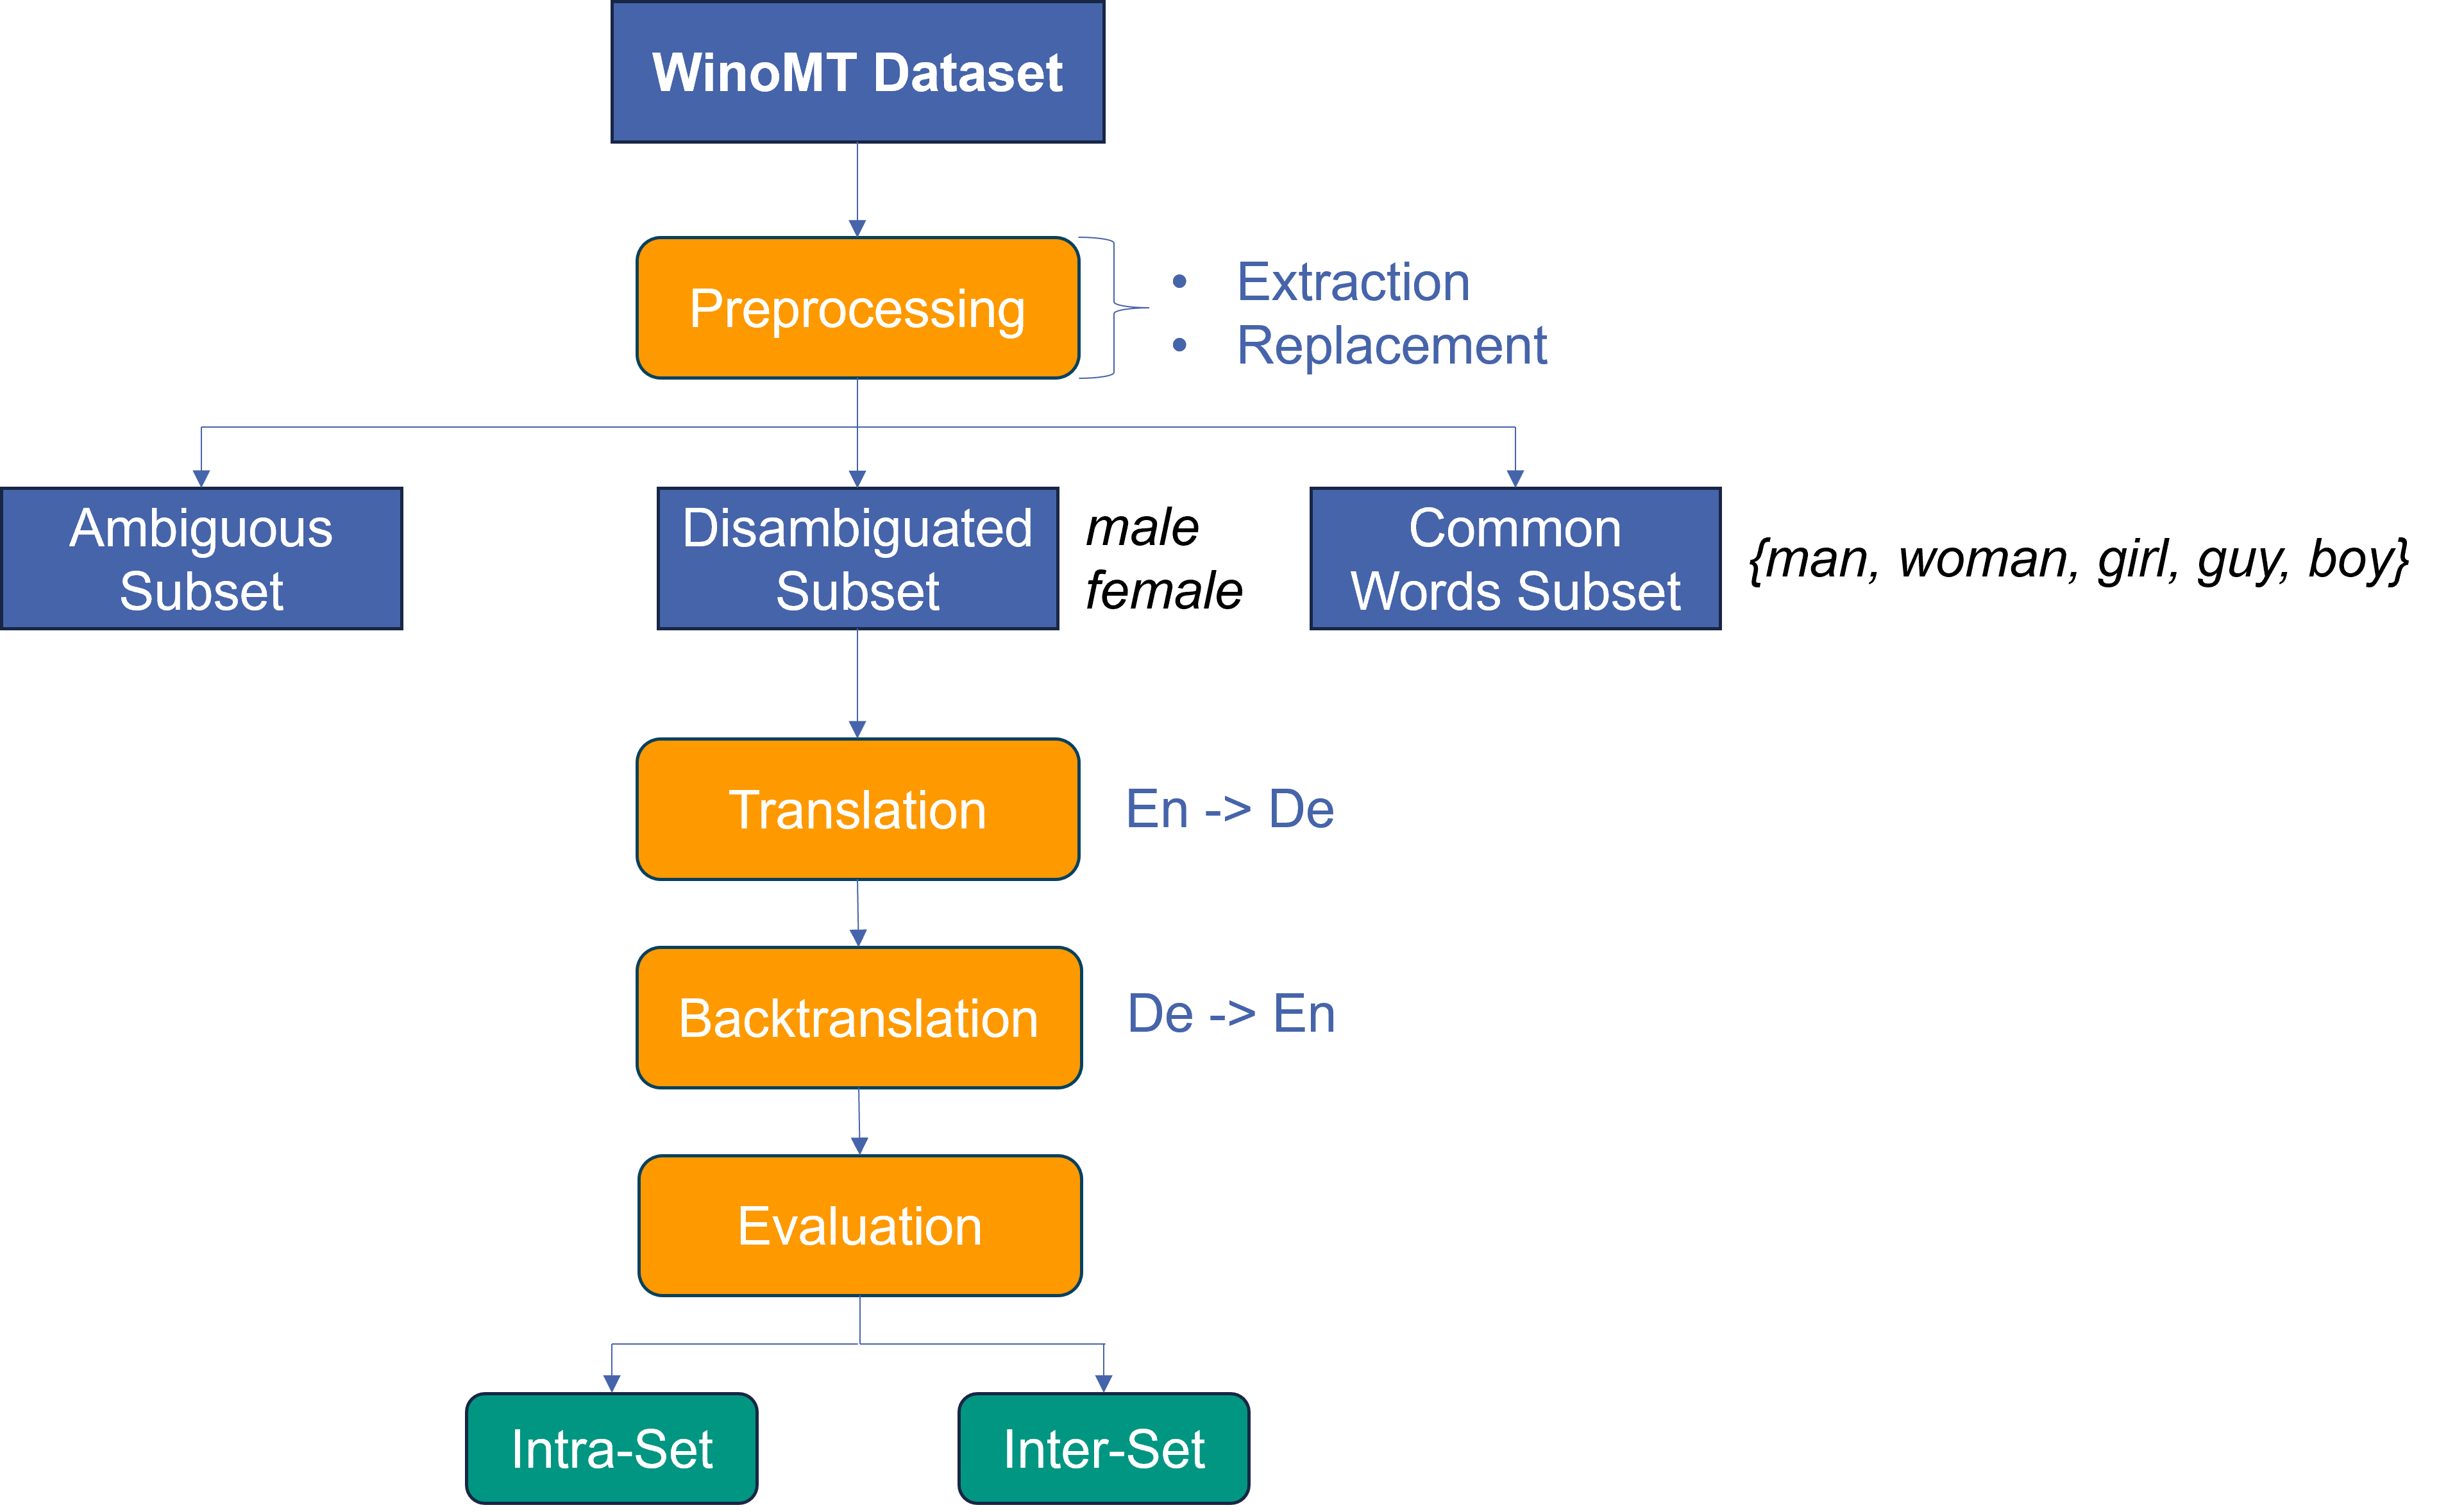
\includegraphics[scale=0.55]{figures/base_workflow.png}
  \caption{Base Experiment Workflow}
  \label{fig:base_workflow}
\end{figure}

%%%%%%%%%%%%%%%%%%%%%%%%%%%%%%%%%%%%%%%%%%%%%%%%%%%%%%%%%%%%%%%%%%%%%%%%%%%%%%%%%%%%%%%%%%%%
\section{Data Pre-processing}
\label{sec:Base_Experiment:Pre-processing}
The first step in conducting the base experiment is preprocessing the dataset. We use the artificially created WinoMT challenge set, presented in Subsection \ref{sec:Setup:Challenge_Set}. The sentences in this dataset usually consist of two gender-ambiguous occupation nouns and a context, containing disambiguation information about one of the occupations. We take the following steps to preprocess the sentences:

\begin{enumerate}
  \item \textbf{Sentence Extraction:}  
  In order to obtain fully ambiguous sentences, we remove the context information from the sentences and obtain a subset of 335 sentences from the type: "The developer argued with the designer.".
  To remove additional detection overhead, we want to have a single ambiguous word per sentence. For this purpose, we replace the second ambiguous word with a non-ambiguous proper noun, e.g., "John". 
  \item \textbf{Replacement:} As next, we generate new subsets of sentences, substituting the ambiguous word in the original sentence with a non-ambiguous version, using two different techniques:
  \begin{itemize}
      \item \textbf{Disambiguation:} We use the gender-defining adjectives \textit{male} and \textit{female} in front of the gender-ambiguous word. This technique is meant to force the translator to make the right decision regarding gender. % gender forcing
      \item \textbf{Common Words:} We replace the ambiguous word with each of the following common gender non-ambiguous words: \textit{man, woman, girl, guy, boy}. We evaluate for each word separately, as well as take the average of them. This method serves as a baseline for comparison against the disambiguated occupation nouns.
  \end{itemize}
\end{enumerate}

Table \ref{tab:preprocessing} shows the generated non-ambiguous subsets obtained by modifying the base ambiguous sentence "The developer argued with John.".

\begin{table}[!htb]
    \begin{tabularx}{\linewidth}{|l|X|l|}
        \hline
        \textbf{Replacement Method} & \textbf{Source Sentence} & \textbf{Source Word} \\ \hline
        \multirow{2}{*}{Disambiguation} & The \textbf{male developer} argued with John. & developer \\
        & The \textbf{female developer} argued with John. & developer \\ \hline
        \multirow{5}{*}{Common Words} & The \textbf{man} argued with John. & man \\
        & The \textbf{woman} argued with John. & woman \\
        & The \textbf{girl} argued with John. & girl \\
        & The \textbf{guy} argued with John. & guy \\
        & The \textbf{boy} argued with John. & boy \\ \hline
    \end{tabularx}
    \caption{\textbf{Example}: Non-ambiguous subsets for the baseline sentence "The developer argued with John.". \\ Source sentence: reflects the sentence in the non-ambiguous subset. \\ Source word: word in the sentence we evaluate for.}
    \label{tab:preprocessing}
\end{table}

The subsets resulting from the preprocessing are: 
\begin{itemize}
    \item \textbf{Ambiguous Subset}: a subset, containing the base ambiguous sentences.
    \item \textbf{Disambiguated Subset (male)}: a subset, containing the sentences, disambiguating the ambiguous word with \textit{male}.
    \item \textbf{Disambiguated Subset (female)}: a subset, containing the sentences, disambiguating the ambiguous word with \textit{female}.
    \item \textbf{Non-ambiguous Subsets}: five subsets, where the ambiguous word is replaced with the common words: \textit{man, woman, girl, guy, boy}.
\end{itemize}



%%%%%%%%%%%%%%%%%%%%%%%%%%%%%%%%%%%%%%%%%%%%%%%%%%%%%%%%%%%%%%%%%%%%%%%%%%%%%%%%%%%%%%%%%%%%
\section{Translation}
\label{sec:Base_Experiment:Translation}

The next step in conducting the experiments is translating the subsets of sentences. We translate from English to German. This is executed in two steps:

\begin{enumerate}
    \item \textbf{Translation Source -> Target:} 
    First, the subsets are translated in the target language (German).
    \item \textbf{Backtranslation Target -> Source:}
    The second step involves translating the translations back into the source language (English).
\end{enumerate}

For the purpose of  translation, we use two different decoding algorithms: Beam search and Sampling (see Subsection \ref{sec:Background:Decoding}). With Beam search, we compare the results for two different beam sizes: 10 and 100. The nbest size is the size of the number of unique translations, generated at each step. 

%%%%%%%%%%%%%%%%%%%%%%%%%%%%%%%%%%%%%%%%%%%%%%%%%%%%%%%%%%%%%%%%%%%%%%%%%%%%%%%%%%%%%%%%%%%%
\section{Word alignment}
\label{sec:Base_Experiment:Alignment}

In order to assign the words in the source sentence to their counterparts in the translations, we use two different alignment methods:

\begin{itemize}
    \item Source-to-translation (\textit{fast\_align}, \textit{awesome-align}): This alignment method aligns from the source language to the target language.
    \item Translation-to-translation (\textit{Tercom}): This alignment method aligns between two translations.
\end{itemize}

We use the first method to map each word in the source sentence to its translations and backtranslations in the target nbest lists. We do this in a two-step way, depicted in Fig. \ref{fig:alignment}. First, we align between the source sentence and the sentences in the nbest translations and extract the translations for each word. Then, we align between the translations and the backtranslations and extract the corresponding backtranslations resulting from the aligned translations of each word. 

We use the results from the second method as a baseline for comparison with the first method and to detect possible errors, which may occur in the information transfer between the two steps in the first method.

\begin{figure}[!htb]
  \centering
  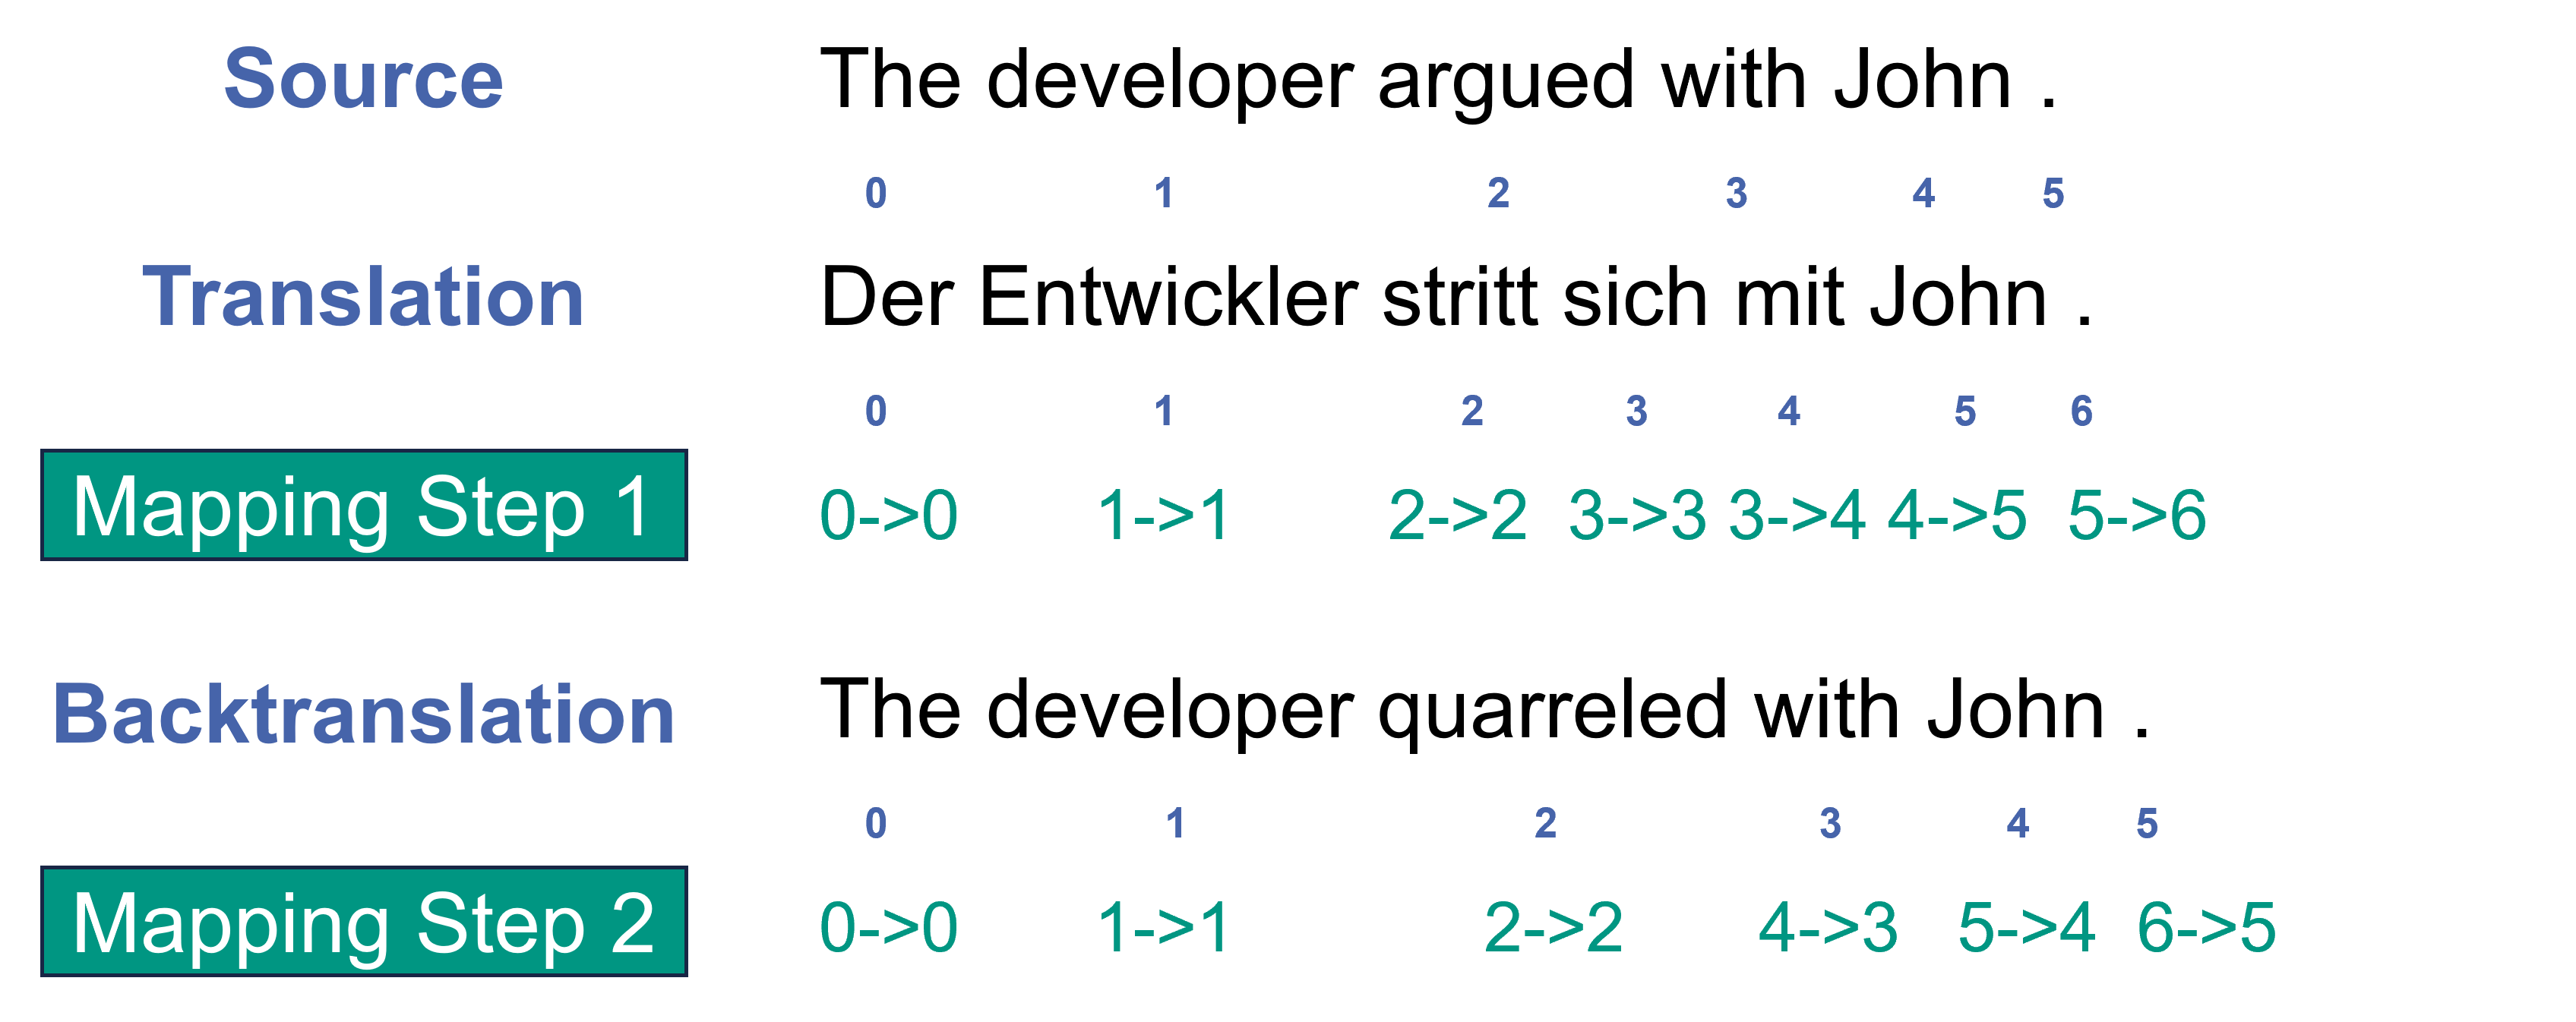
\includegraphics[scale=0.5]{figures/alignment.png}
  \caption{Example Illustration: 2-step mapping from source to translation and backtranslation}
  \label{fig:alignment}
\end{figure}

%%%%%%%%%%%%%%%%%%%%%%%%%%%%%%%%%%%%%%%%%%%%%%%%%%%%%%%%%%%%%%%%%%%%%%%%%%%%%%%%%%%%%%%%%%%%
\section{Evaluation}
\label{sec:Base_Experiment:Evaluation}

The last step in the experiments involves evaluating the translations and backtranslations to detect patterns using different statistical methods. These methods aim to probe the initial Hypothesis \ref{main}, discussed in Section \ref{sec:Methodology:Approach}. We apply all methods to all subsets, as presented in Section \ref{sec:Base_Experiment:Pre-processing}, and extract diversity information regarding the subsets themselves, as well as compare the results of the subsets against each other.

% define formally, maybe as a formula, pseudocode ???

%%%%%%%%%%%%%%%%%%%%%%%%%%%%%%%%%%%%%%%%%%%%%%%%%
\subsection{Reoccurrence Evaluation}
\label{sec:Base_Experiment:Statistics:Reoccurrence}
We evaluate how many of the source sentences and source words reoccur in the backtranslations:

\begin{enumerate}
    \item[1. ] Gather the backtranslations for each source sentences.
    \item[2a. ] Count the number of source sentences that reappear in their list of backtranslations.
    \item[2b. ] Count the number of source sentences which contain the source word in their backtranslations.
\end{enumerate}

% Is it to test which disambiguation method is better?
The purpose of this evaluation is to determine which of the subsets are able to reconstruct more of the source sentences/words. This could indicate which disambiguation method does better in restoring the original sentence. 

We also evaluate how often the source sentences and source words reoccur in the backtranslations:

\begin{enumerate}
    \item[1. ] Gather the backtranslations for each source sentences.
    \item[2a. ] Count in how many of the backtranslations the source sentences reappear.
    \item[2b. ] Count in how many of the backtranslations the source word reappears.
\end{enumerate}

We use this method to probe the Hypotheses \ref{d}. 

%%%%%%%%%%%%%%%%%%%%%%%%%%%%%%%%%%%%%%%%%%%%%%%%%
\subsection{Uniqueness Evaluation}
\label{sec:Base_Experiment:Statistics:Uniqueness}
We evaluate the number of unique words and sentences in the translations and backtranslations for each sentence of the subsets. 

For the sake of the evaluation, we follow this routine (\textit{[translations | backtranslations]} denotes that we follow the same step for both the translations and backtranslations):
\begin{enumerate}
    \item[1. ] Collect the \textit{[translations | backtranslations]} for each source sentences.
    % sentence level
    \item[2a. ] Count how many of the \textit{[translations | backtranslations]} are unique. 
    % word level
    \item[2b. ] Count how many unique words there are in the \textit{[translations | backtranslations]} and normalize the number by the total amount of words. 
    \item[3. ] Average the result for all sentences.
\end{enumerate}

We use this method to probe the Hypotheses \ref{a} and \ref{b}. 

%%%%%%%%%%%%%%%%%%%%%%%%%%%%%%%%%%%%%%%%%%%%%%%%%
\subsection{Gender Evaluation}
\label{sec:Base_Experiment:Statistics:Gender}
We perform the evaluation of gender on the translations of the subsets.  First, we align each word in the source sentence with its corresponding word in the translations and backtranslations (see Subsection \ref{sec:Base_Experiment:Alignment} for more detail). Then, we perform the following steps:

\begin{enumerate}
    \item[1. ] Gather the translations of the source word for each source sentence.
    \item[2. ] Detect the gender of the translations for each source sentence.
    \item[3a. ] Determine the proportion of source sentences producing \textit{male} versus \textit{female}.
    \item[3b. ] Calculate how many of the source sentences produce \textit{both genders}. 
\end{enumerate}

The purpose of this method is to assess if the translations produce the right gender (in the non-ambiguous subsets) or both genders (in the ambiguous subset) and how often they produce both genders for each subset.

%%%%%%%%%%%%%%%%%%%%%%%%%%%%%%%%%%%%%%%%%%%%%%%%%
\subsection{Alignment Evaluation}
\label{sec:Base_Experiment:Statistics:Alignment}
Another form of evaluation is based on the alignment of the words between the source sentence, the translations and backtranslations (see Subsection \ref{sec:Base_Experiment:Alignment} for more detail).

In order to assess the translations and backtranslations of the \textbf{source word}, we do:
\begin{enumerate}
    \item[1. ] Collect all \textit{[translations | backtranslations]} of the source word.
    \item[2. ] Count how many of the \textit{[translations | backtranslations]} are unique.
    \item[3. ] Average the result for all sentences.
\end{enumerate}

Similarly, to assess the translations and backtranslations of the \textbf{rest of the sentence} excluding the source word, we do:
\begin{enumerate}
    \item[1. ] Collect all \textit{[translations | backtranslations]} of the sentence rest.
    \item[2. ] Count how many of the \textit{[translations | backtranslations]} are unique.
    \item[3. ] Average the result for all sentences.
\end{enumerate}

The idea behind this evaluation method is to assess the Hypothesis \ref{c}.

Next, we will present the results of these statistical evaluations of the subsets.

%%%%%%%%%%%%%%%%%%%%%%%%%%%%%%%-----------------------------%%%%%%%%%%%%%%%%%%%%%%%%%%%%%%%%%%%%%%%
\section{Results}
\label{ch:Base_Experiment:Results}

% - Translation quality
% BLEU score on WinoMT: not possible, because no reference translations
% - Gender bias quality

We evaluate the translations and backtranslations of the different subsets based on the presented evaluation methods and present the results in the following subsections.

%%%%%%%%%%%%%%%%%%%%%%%%%%%%%%%%%%%%%%%%%%%%%%%%%
\subsection{Reoccurrence Evaluation Results}
\label{ch:Base_Experiment:Results:Reoccurrence}

\begin{table}[!htb] 
    \begin{subtable}{\textwidth}
        \centering
        \begin{tabularx}{\linewidth}{|X|XXXX|}
            \hline
             & \textbf{Ambiguous} & \textbf{Disambiguated (male)} & \textbf{Disambiguated (female)} & \textbf{Non-ambiguous average} \\ \hline
             \textbf{\#Sentences} & 295/335 & 293/335 & 118/335 & \underline{308/335} \\
             \textbf{\#Sentences (R)} & 295/335 & 6/335 & 25/335 & \underline{308/335} \\ 
             \textbf{Sentences } & 6.5/100 & 4.72/100 & 1.13/100 & \underline{6.69/100} \\ \hline
             \textbf{\#Words} & 329/335 & 330/335 & 314/335 & \underline{335/335} \\ 
             \textbf{\#Words (R)} & 329/335 & 330/335 & 314/335 & \underline{335/335} \\ 
             \textbf{Words} & 56.65/100 & 58.8/100 & 50.47/100 & \underline{71.26/100} \\ \hline
        \end{tabularx}
        \subcaption{\textbf{Beam search with beam size 10}. Backtranslation. Nbest size 10. Highest scores are underlined. \textbf{R}: removed German words for \textit{male} and \textit{female}. \\ First and second row: number of source sentences that reappear in the backtranslations. \\ Third row: averaged number of times the source sentences reoccur in 100 backtranslations. \\ Fourth and fifth row: number of source sentences which contain the source word in the backtranslations. \\ Sixth row: averaged number of times the source words reoccur in 100 backtranslations.}
        \label{tab:reoccurrence_10}
    \end{subtable}
    
    \begin{subtable}{\textwidth}
        \centering
        \begin{tabularx}{\linewidth}{|X|XXXX|}
            \hline
             & \textbf{Ambiguous} & \textbf{Disambiguated (male)} & \textbf{Disambiguated (female)} & \textbf{Non-ambiguous average} \\ \hline
             \textbf{\#Sentences} & 329/335 & \underline{330/335} & 281/335 & 329/335 \\ 
             \textbf{Sentences} & 72.51/10000 & 48.59/10000 & 21.85/10000 & \underline{70.94/10000} \\ \hline
             \textbf{\#Words} & 335/335 & 335/335 & 335/335 & 335/335 \\
             \textbf{Words} & 4714.74/10000 & 4788.99/10000 & 4192.54/10000 & \underline{5925.98/10000} \\ \hline
        \end{tabularx}
        \subcaption{\textbf{Beam search with beam size 100}. Backtranslation. Nbest size 100. Highest scores are underlined. \\ First row: number of source sentences that reappear in the backtranslations. \\ Second row:  averaged number of times the source sentences reoccur in 10000 backtranslations. \\ Third row: number of source sentences which contain the source word in the backtranslations. \\ Fourth row: averaged number of times the source words reoccur in 10000 backtranslations.}
        \label{tab:reoccurrence_100}
    \end{subtable}

    \begin{subtable}{\textwidth}
        \centering
        \begin{tabularx}{\linewidth}{|X|XXXX|}
            \hline
             & \textbf{Ambiguous} & \textbf{Disambiguated (male)} & \textbf{Disambiguated (female)} & \textbf{Non-ambiguous average} \\ \hline
             \textbf{\#Sentences} & 270/335 & 249/335 & 87/335 & \underline{295/335} \\ 
             \textbf{Sentences} & 3.99/100 & 2.52/100 & 0.58/100 & \underline{4.54/100} \\ \hline
             \textbf{\#Words} & 332/335 & 333/335 & 326/335 & \underline{335/335} \\
             \textbf{Words} & 50.83/100 & 49.02/100 & 43.86/100 & \underline{66.83/100} \\ \hline
        \end{tabularx}
        \subcaption{\textbf{Sampling}. Backtranslation. Nbest size 10. Highest scores are underlined. \\ First row: number of source sentences that reappear in the backtranslations. \\ Second row:  averaged number of times the source sentences reoccur in 100 backtranslations. \\ Third row: number of source sentences which contain the source word in the backtranslations. \\ Fourth row: averaged number of times the source words reoccur in 100 backtranslations.}
        \label{tab:reoccurrence_sampling}
    \end{subtable}
    
    \caption{Reoccurrence Evaluation Results}
    \label{tab:reoccurrence}
\end{table}

The results from the evaluation of reoccurrence are listed in Table \ref{tab:reoccurrence}.
% Highest score
As we can observe, the average from the subsets of common words dominates the highest score in both the recurring sentences and words. This is to be expected, because the words in these subsets are most generic and have the highest probability of being predicted, compared to the occupational words from the WinoMT sentences in the other three subsets. 

% Interesting findings
Most interestingly, the female-disambiaguated subset has the lowest score for reoccurring sentences. When investigating the results, we found some discrepancy between the way "female" and "male" are translated. The "female" prefix is very often lost in the backtranslation, which results in the backtranslated sentence being regarded as differing from the source sentence. In contrast, the "male" prefix is most often preserved, resulting in the same sentence in backtranslation. We illustrate this with the following examples:

\begin{itemize}
    \item \textbf{Source (EN):} The \textit{female} developer argued with John. \\
    \textbf{Translation (DE):} Die Entwicklerin argumentierte mit John. \\
    \textbf{Backtranslation (EN):} The developer argued with John.
    
    \item \textbf{Source (EN):} The \textit{male} developer argued with John. \\
    \textbf{Translation (DE):} Der \textit{männliche} Entwickler argumentierte mit John. \\
    \textbf{Backtranslation (EN):} The \textit{male} developer argued with John.
\end{itemize}

As we can see, the "male" prefix is translated to its corresponding word in German "männliche", while the "female" prefix is lost in the translation, but its meaning is reflected in the female gender of the German word for developer "Entwicklerin".

Also, both disambiguation subsets sometimes generate the opposite gender with the correct prefix, for example, "der \textit{weibliche} Entwickler" (the \textit{female} male developer) and "die \textit{männliche} Entwicklerin" (the \textit{male} female developer). This presents a contradiction that influences the translation quality. We tried mitigating this by removing the German words for "female" and "male" from the translations with Beam search with beam size 10 (see Table \ref{tab:reoccurrence_10}). As we can see, this has a significant effect on the reoccurrence in backtranslation for the disambiguated subsets. For the male-disambiguated subset, only 6 out of 335 sentences reoccur, while for the female-disambiguated subset 25 out of 335 sentences reoccur. The conclusion we can make from these results is that the gender prefix words "male" and "female" most often reappear in backtranslation, when they are initially translated to their German counterpart, and when this is not the case, they are less likely to be reproduced in backtranslation for male than for female.

We note that the findings from these results are important and will have an effect on the further experiments.

% Beam size 100
Table \ref{tab:reoccurrence_100} shows the results from the evaluation of reoccurrence for beam search with beam size 100. Here we can observe that more female sentences are reoccurring in backtranslation compared to beam 100, which means that increasing the beam increases the possibility for preservation of the "female" prefix in the backtranslations. Also, with beam size 100 the source word reappears for all source sentences in the backtranslations.

% Hypothesis d); Sampling
The results from Sampling, as seen in Table \ref{tab:reoccurrence_sampling}, show that the ambiguous word reoccurs more often in backtranslations than the corresponding disambiguated words (male and female), which was not the case with Beam search. Although the non-ambiguous word still reoccurs most often, this is a positive result for Hyp. \ref{d}.

%%%%%%%%%%%%%%%%%%%%%%%%%%%%%%%%%%%%%%%%%%%%%%%%%
\subsection{Uniqueness Evaluation Results}
\label{ch:Base_Experiment:Results:Uniqueness}

The results from the evaluation of uniqueness are listed in Table \ref{tab:uniqueness_translation} for translation and Table \ref{tab:uniqueness_backtranslation} for backtranslation.
Since we use the beam search algorithm for decoding with beam size 10 and nbest size 10, we expect it to generate 10 unique sentences per translation, which is almost always the case, as we see from the score for the number of unique sentences in translations. With Sampling, we sample a higher number of translations, and extract 10 unique translations from the generated samples.

% Table for Translation
\begin{table}[!htb]

    \begin{subtable}{\textwidth}
        \centering
        \begin{tabularx}{\linewidth}{|X|XXXX|}
            \hline
             & \textbf{Ambiguous} & \textbf{Disambiguated (male)} & \textbf{Disambiguated (female)} & \textbf{Non-ambiguous average} \\ \hline
             \textbf{Sentences} & 9.94/10 & 9.95/10 & 9.87/10 & \underline{9.97/10} \\ 
             \textbf{Words} & \underline{0.205} & 0.19 & 0.201 & 0.202 \\ \hline
        \end{tabularx}
        \caption{\textbf{Beam search with beam size 10}. Nbest size 10. Highest scores are underlined. \\ First row: Averaged number of unique sentences per source sentence out of 10 translations. \\ Second row: Averaged number of unique words per source sentence, normalized by the average total number of words in 10 translations.}
        \label{tab:uniqueness_translation_10}
    \end{subtable}

    \begin{subtable}{\textwidth}
        \centering
        \begin{tabularx}{\linewidth}{|X|XXXX|}
            \hline
             & \textbf{Ambiguous} & \textbf{Disambiguated (male)} & \textbf{Disambiguated (female)} & \textbf{Non-ambiguous average} \\ \hline
             \textbf{Sentences} & 10/10 & 10/10 & 10/10 & 10/10 \\ 
             \textbf{Words} & 0.278 & 0.277 & \underline{0.29} & 0.263 \\ \hline
        \end{tabularx}
        \caption{\textbf{Sampling}. Nbest size 10. Highest scores are underlined. \\ First row: Averaged number of unique sentences per source sentence out of 10 translations. \\ Second row: Averaged number of unique words per source sentence, normalized by the average total number of words in 10 translations.}
        \label{tab:uniqueness_translation_sampling}
    \end{subtable}
    \caption{\textbf{Uniqueness Evaluation Results for Translation}}
    \label{tab:uniqueness_translation}
\end{table}

% Table for Backtranslation
\begin{table}[!htb] 

    \begin{subtable}{\textwidth}
        \centering
        \begin{tabularx}{\linewidth}{|X|XXXX|}
            \hline
             & \textbf{Ambiguous} & \textbf{Disambiguated (male)} & \textbf{Disambiguated (female)} & \textbf{Non-ambiguous average} \\ \hline
             \textbf{Sentences} & 45.98/100 & 50.73/100 & \underline{50.82/100} & 47.06/100 \\
             \textbf{Sentences (R)} & 45.98/100 & 41.36/100 & 47.03/100 & \underline{47.06/100} \\ \hline
             \textbf{Words} & 0.044 & 0.039 & 0.043 & \underline{0.045} \\ 
             \textbf{Words (R)} & 0.044 & 0.042 & 0.043 & \underline{0.045} \\ \hline
        \end{tabularx}
        \caption{\textbf{Beam search with beam size 10}. Nbest size 10. \\ Highest scores are underlined. \textbf{R}: removed German words for \textit{male} and \textit{female}. \\ First and second row: Averaged number of unique sentences per source sentence out of 10 translations. \\ Third and fourth row: Averaged number of unique words per source sentence, normalized by the average total number of words in 100 backtranslations.}    
        \label{tab:uniqueness_backtranslation_10}
    \end{subtable}

    \begin{subtable}{\textwidth}
        \centering
        \begin{tabularx}{\linewidth}{|X|XXXX|}
            \hline
             & \textbf{Ambiguous} & \textbf{Disambiguated (male)} & \textbf{Disambiguated (female)} & \textbf{Non-ambiguous average} \\ \hline
             \textbf{Sentences} & 3181.51/10000 & 3391.55/10000 & \underline{3424.98/10000} & 3297.48/10000 \\ \hline
        \end{tabularx}
        \caption{\textbf{Beam search with beam size 100}. Nbest size 100. \\ Highest scores are underlined. Averaged number of unique sentences per source sentence out of 100 translations.}
        \label{tab:uniqueness_backtranslation_100}
    \end{subtable}

    \begin{subtable}{\textwidth}
        \centering
        \begin{tabularx}{\linewidth}{|X|XXXX|}
            \hline
             & \textbf{Ambiguous} & \textbf{Disambiguated (male)} & \textbf{Disambiguated (female)} & \textbf{Non-ambiguous average} \\ \hline
             \textbf{Sentences} & 81.81/100 & \underline{86.87/100} & 85.75/100 & 80.6/100 \\ 
             \textbf{Words} & 0.104 & 0.103 & \underline{0.108} & 0.098 \\ \hline
        \end{tabularx}
        \caption{\textbf{Sampling}. Nbest size 10. \\ Highest scores are underlined. \\ First row: Averaged number of unique sentences per source sentence out of 10 translations. \\ Third row: Averaged number of unique words per source sentence, normalized by the average total number of words in 100 backtranslations.}
        \label{tab:uniqueness_backtranslation_sampling}
    \end{subtable}

    \caption{\textbf{Uniqueness Evaluation Results for Backtranslation}}
    \label{tab:uniqueness_backtranslation}
\end{table}

%%% Range of uniqueness
\begin{figure}[!htb]
     \centering
     
     \begin{subfigure}{0.49\textwidth}
         \centering
         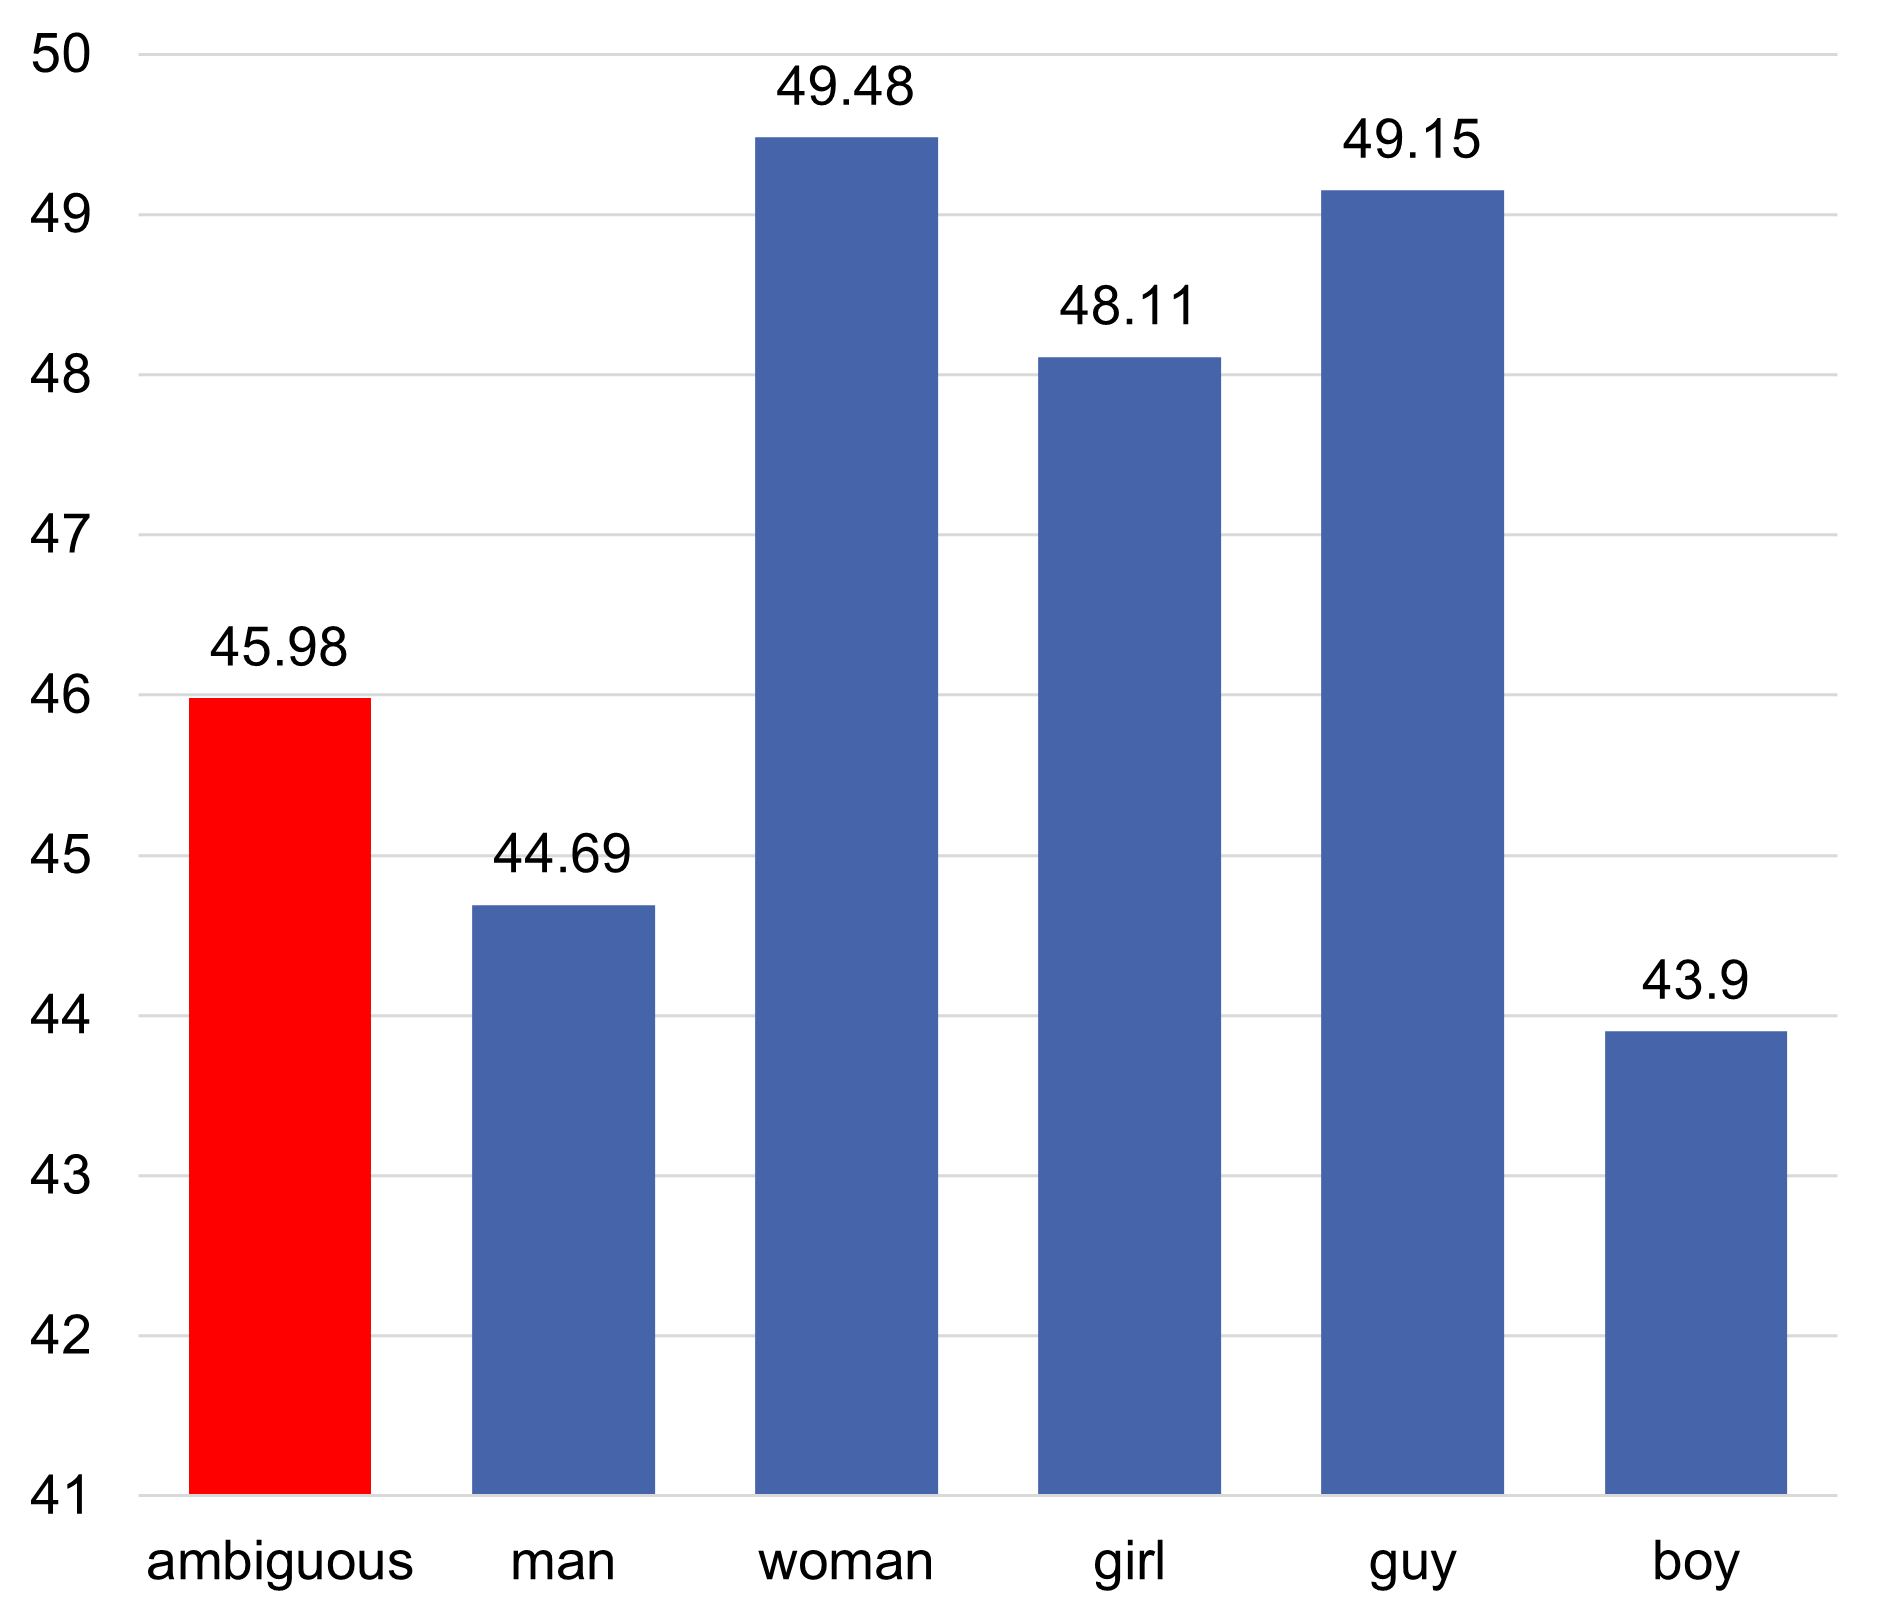
\includegraphics[width=\textwidth]{figures/uniqueness/range_beam_10.png}
         \caption{Beam search with beam size 10}
         \label{fig:uniqueness_range_10}
     \end{subfigure}
     \hfill
     \begin{subfigure}{0.49\textwidth}
         \centering
         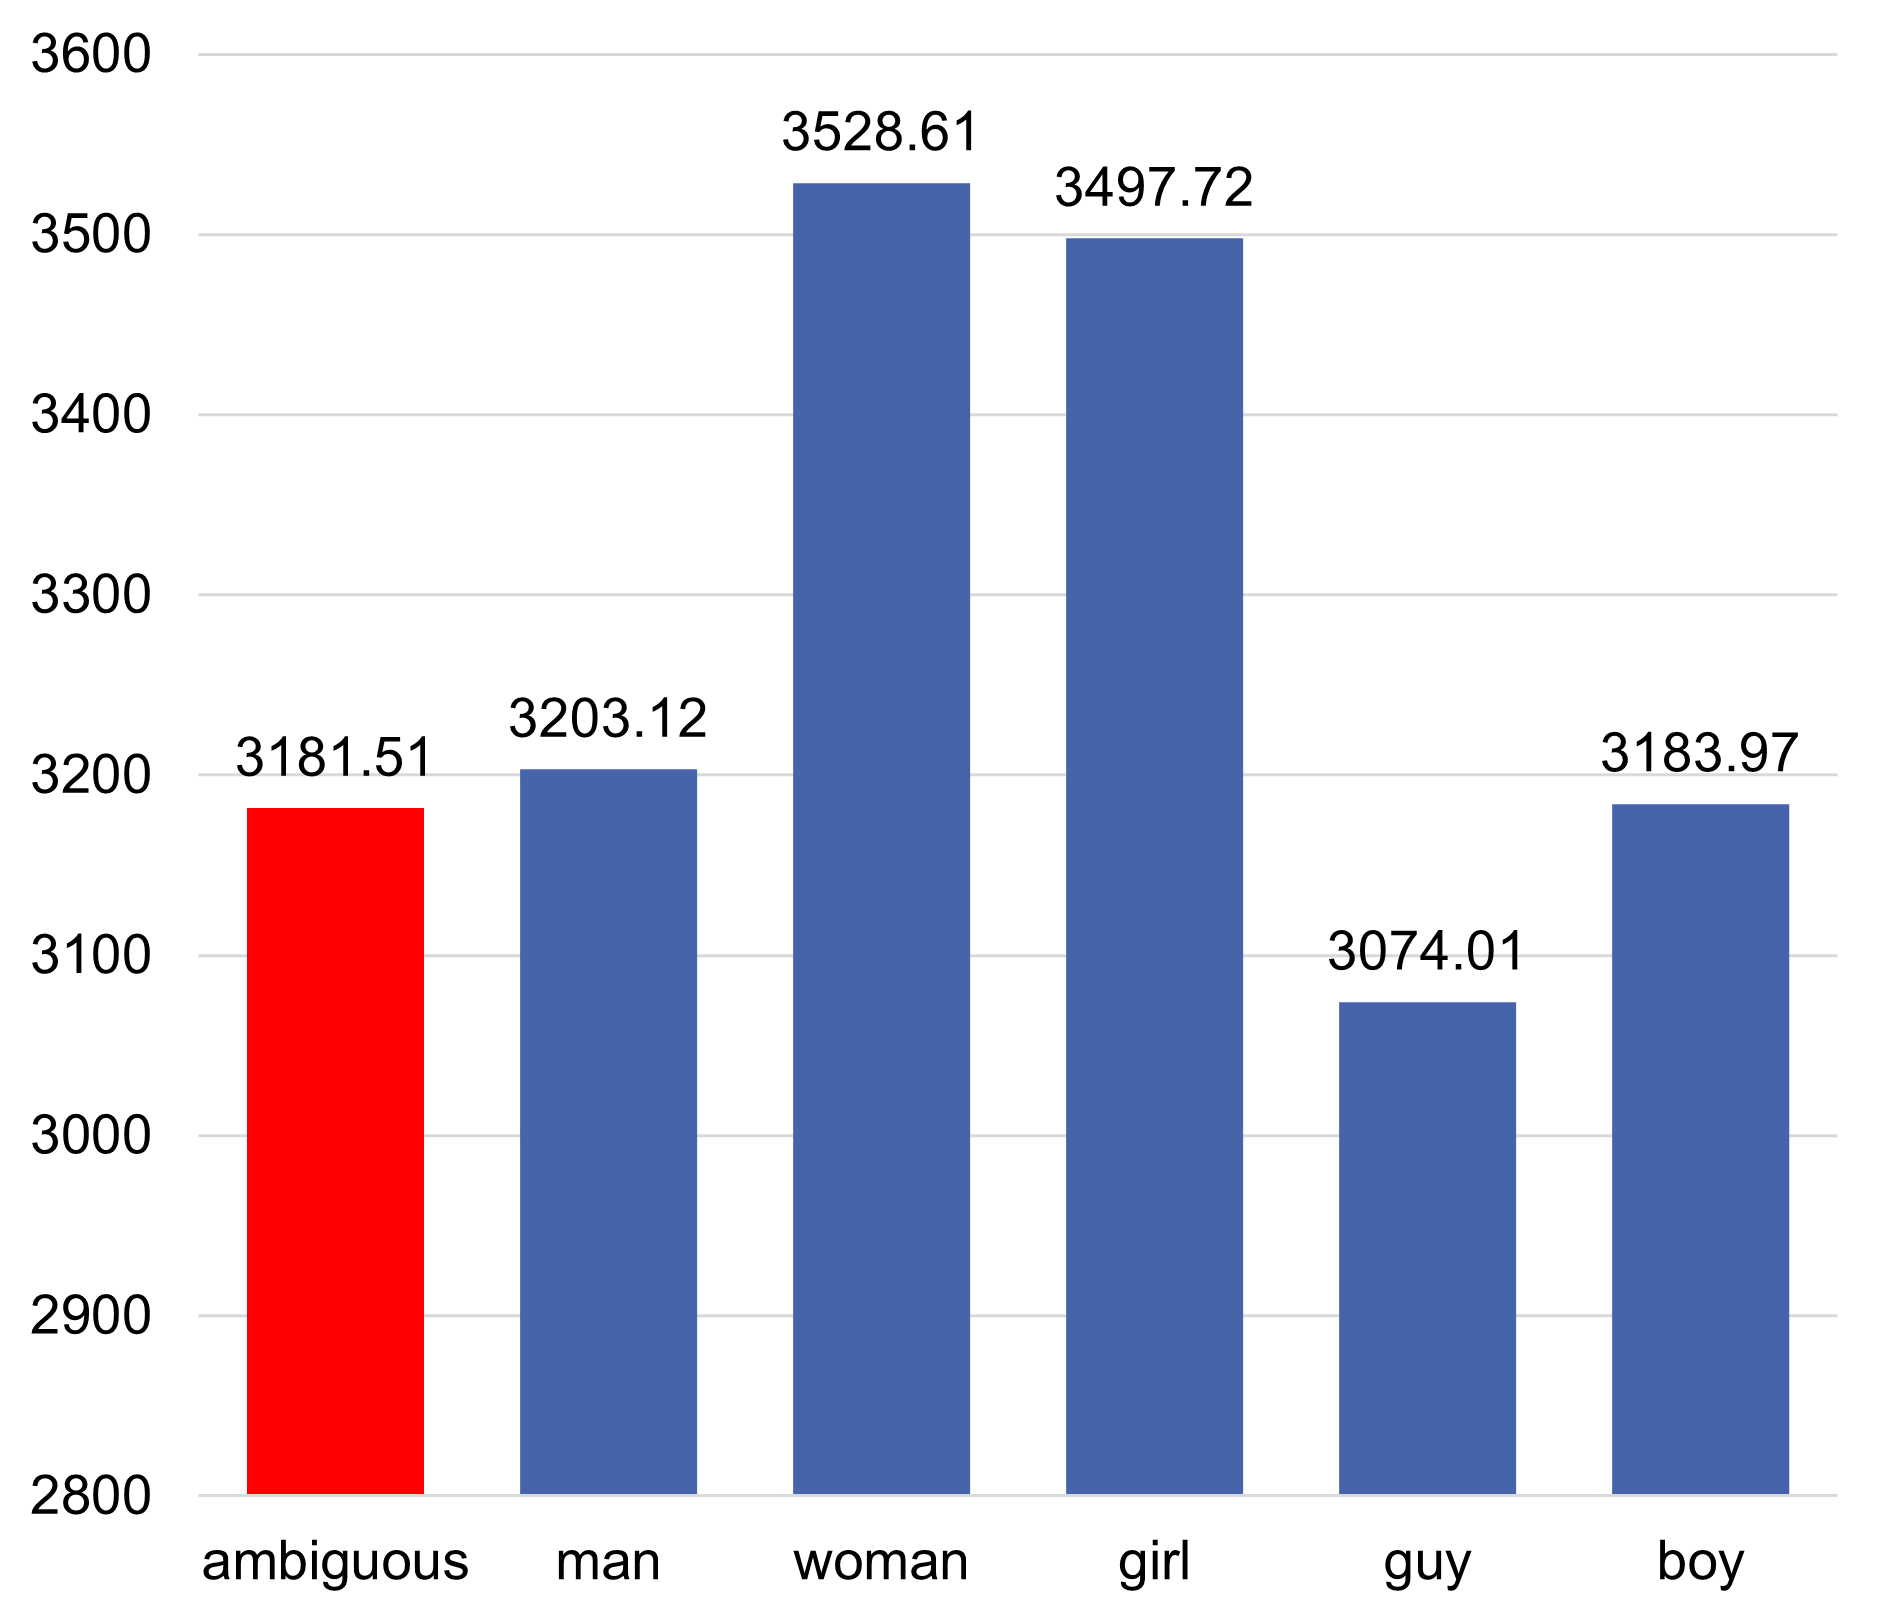
\includegraphics[width=\textwidth]{figures/uniqueness/range_beam_100.png}
         \caption{Beam search with beam size 100}
         \label{fig:uniqueness_range_100}
     \end{subfigure}
     
    \caption{Comparison Between the Number of Unique Backtranslations for Common Words and Ambiguous Subsets}
    \label{fig:uniqueness_range}

\end{figure}

% Graphs
\begin{figure}[!htb]
     \centering
     
     \begin{subfigure}{0.49\textwidth}
         \centering
         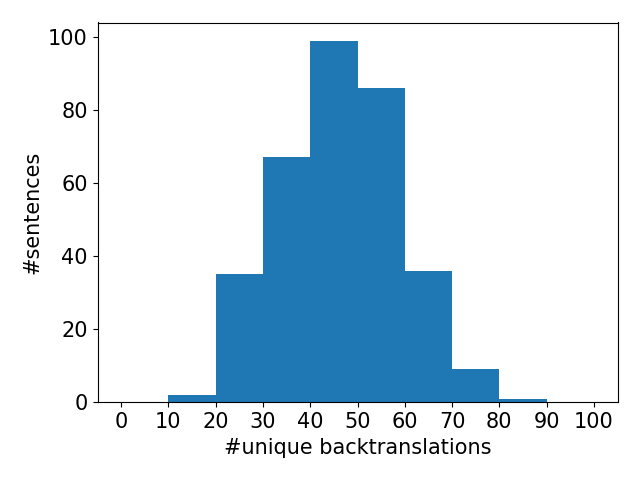
\includegraphics[width=\textwidth]{figures/uniqueness/unique_beam10/unique_back_original.png}
         \caption{Ambiguous Subset}
         \label{fig:uniqueness_ambiguous}
     \end{subfigure}
     \hfill
     \begin{subfigure}{0.49\textwidth}
         \centering
         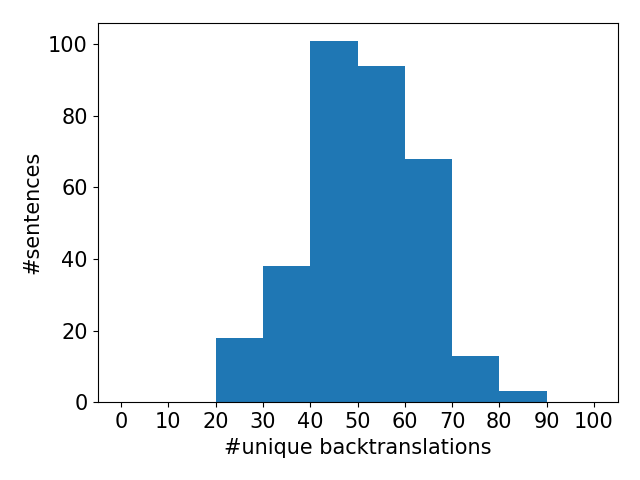
\includegraphics[width=\textwidth]{figures/uniqueness/unique_beam10/unique_back_male.png}
         \caption{Disambiguated Subset (male)}
         \label{fig:uniqueness_male}
     \end{subfigure}
     \begin{subfigure}{0.49\textwidth}
         \centering
         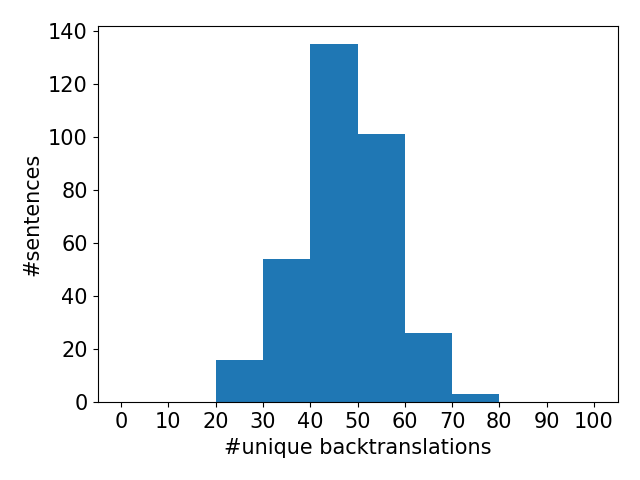
\includegraphics[width=\textwidth]{figures/uniqueness/unique_beam10/unique_back_average.png}
         \caption{Non-ambiguous Subset Average}
         \label{fig:uniqueness_common}
     \end{subfigure}
     \hfill
     \begin{subfigure}{0.49\textwidth}
         \centering
         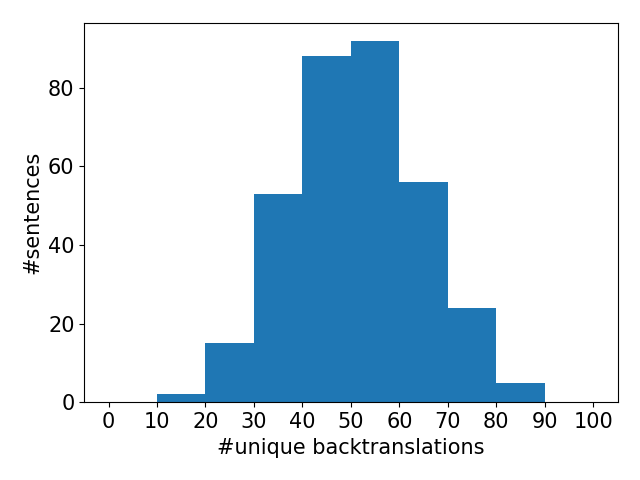
\includegraphics[width=\textwidth]{figures/uniqueness/unique_beam10/unique_back_female.png}
         \caption{Disambiguated Subset (female)}
         \label{fig:uniqueness_female}
     \end{subfigure}
        \caption{Distribution of Unique Backtranslations: Beam search with beam size 10}
        \label{fig:uniqueness_graphs_10}

\end{figure}

% Interesting findings
Most notable are the results for the number of unique backtranslations. As we can see in the first row of Table \ref{tab:alignment_backtranslation_10}, the ambiguous subset produces the least amount of unique sentences in backtranslation, which proves Hyp. \ref{a}. To inspect this further, we increase the beam size to 100, and as we see from Table \ref{tab:uniqueness_backtranslation_100} this experiment confirms the results.

However, when removing the German prefix gender words \textit{male} and \textit{female} we get mixed results in relation to the disambiguated subsets. The value for the male-disambiguation is the lowest, however the value for the ambiguous subset is still lower than the female-disambiguated subset. Then, we can speculate that modifying the translation in the suggested manner would not be further useful to the inspection of the approach.

% Range
To investigate this further, we regard the results for the different common words separately instead of averaged, as we can see in Fig. \ref{fig:uniqueness_range}. The minimum value in the range, 43.9 (for the word "boy") for beam size 10 and 3074.01 (for the word "guy") for beam size 100, is still lower for the common words compared to the ambiguous subset, 45.98 for beam size 10 and 3181.51 for beam size 100.

The results for the number of unique words in translation and backtranslation are inconclusive. Considering Hyp. \ref{b}, we expected the ambiguous subset to generate the least unique words in backtranslation, but this is not the case.

% Sampling
We also investigated the generated backtranslations from the Sampling method, as seen in \ref{tab:uniqueness_backtranslation_sampling}. Interestingly, Sampling generates almost twice as many unique backtranslations, reagrding both words and sentences. Here, the lowest score belongs to the non-ambiguous subset, contrary to the expectation from Hyp. \ref{a}. However, the ambiguous subset still has less unique backtranslations than the corresponding disambiguated subsets, which is what we expect.

% Distribution graphs
Furthermore, we plot the distribution of unique backtranslations, which can be seen in Fig. \ref{fig:uniqueness_graphs_10} for Beam search with beam size 10, containing the histograms for each subset. 
Most sentences have between 40 and 50 unique backtranslations , except for the female-disambiguated subset, which have between 50 and 60 unique backtranslations, confirming the highest score from Table \ref{tab:uniqueness_backtranslation}. Another observation we can make pertains to the difference between the ambiguous subset \ref{fig:uniqueness_ambiguous} and the non-ambiguous subset averaged for the common words (\ref{fig:uniqueness_common}). There, we can see that the range is smaller ([20, 80]) and more of the non-ambiguous sentences have the average amount of unique backtranslations (around 140 sentences), while the ambiguous sentences produce more variable amount of backtranslations in terms of range  ([10, 90]) but less amount of sentences producing the average amount of unique backtranslations (around 100 sentences).
The distribution of unique backtranslations for Beam search with beam size 100 and Sampling show the same trend and can be seen in Appendix \ref{chap:appendix}.

As next, we want to inspect the uniqueness of translation for the source word separately.

%%%%%%%%%%%%%%%%%%%%%%%%%%%%%%%%%%%%%%%%%%%%%%%%%
\subsection{Gender Evaluation Results}
\label{ch:Base_Experiment:Results:Gender}

% Male and female
The results from the evaluation of gender are listed in Table \ref{tab:gender_percent_10} for Beam search with beam size 10, Table \ref{tab:gender_percent_100} for Beam search with beam size 100 and Table \ref{tab:gender_percent_sampling} for Sampling. We can observe that, as expected, the subset of disambiguated with "male" sentences has predominantly male translations, and similarly the subset of disambiguated with "female" sentences has mostly female translations. The same applies to the male words "man", "guy" and "boy", as well as the female word "woman". The female word "girl" presents an exception, because in German it is a neutral noun.

Interestingly, when comparing the disambiguation subsets, the disambiguation with "female" seems to be more successful overall, with more sentences producing the right gender and less of both genders appearing in the translations.

% Both genders
Also, as expected, the ambiguous source sentences produce the most translations of both genders, while the common non-ambiguous words produce the least. Despite this, the disambiguation subsets still have a rather high amount of sentences producing both genders. With Sampling, a higher amount of sentences produce both genders of the source word in translations than with Beam search, which point to Sampling producing more variable output in translations.

Furthermore, we can make the observation that a significantly higher percentage of generated translation are male (86.27\% for Beam search, 80.54\% for Sampling) versus female (12.81\% for Beam search, 14.33\% for Sampling). Sampling seems to produce more balanced translations in terms of female versus male, but it is still predominantly male translations of the source word. This can only point to the already biased pre-trained NMT model. 

% Pie 
Fig. \ref{fig:gender_pie_10} further shows the influence of increasing the beam size tenfold and the difference between Beam search and Sampling. We can observe that more of both genders occur in translation of the ambiguous subset with beam size 100 compared to beam size 10. But this is also the case for the disambiguated subsets, where we do not expect this. Also, there is more balance between female and male in the translations of the ambiguous subset, with the difference between 78.66\% and 14.88\% being smaller than between 86.27\% and 12.81\%. But on the other hand, more male gender translations occur in the female-disambiguated subset, which is a downside. Sampling, on the other hand, achieves more balance between male and female without increasing the amount of both genders prediction in the disambiguated subsets, unlike Beam search with beam size 100.

\begin{table}[!htb]

    \begin{subtable}{\textwidth}
        \centering
        \begin{tabularx}{\linewidth}{|X|XXXX|}
            \hline
             & \textbf{Ambiguous} & \textbf{Disambiguated (male)} & \textbf{Disambiguated (female)} & \textbf{Non-ambiguous} \\ \hline
             \textbf{Male} & 86.27\% & 89.46\% & 6.81\% & \textit{man}: 95.01\% \\
             &&&& \textit{woman}: 0.51\% \\
             &&&& \textit{girl}: 0.39\% \\
             &&&& \textit{guy}: 93.07\% \\
             &&&& \textit{boy}: \underline{96.15\%} \\ \hline
             \textbf{Female} & 12.81\% & 11.19\% & 92.33\% & \textit{man}: 0.18\% \\ 
             &&&& \textit{woman}: \underline{96.69\%} \\
             &&&& \textit{girl}: 0.81\% \\
             &&&& \textit{guy}: 0.18\% \\
             &&&& \textit{boy}: 0.27\% \\\hline
             \textbf{Both genders} & \underline{38.21\%} & 35.22\% & 28.06\% & average: 0.72\% \\ \hline
        \end{tabularx}
        \caption{\textbf{Beam search with beam size 10}. Translation. Nbest size 10. Highest scores are underlined. \\ First and second row: Percentage of the source sentences producing male versus female translations. \\ Third row: Percentage of the source sentences producing both genders in translation.}
        \label{tab:gender_percent_10}
    \end{subtable}

    \begin{subtable}{\textwidth}
        \centering
        \begin{tabularx}{\linewidth}{|X|XXXX|}
            \hline
             & \textbf{Ambiguous} & \textbf{Disambiguated (male)} & \textbf{Disambiguated (female)} & \textbf{Non-ambiguous} \\ \hline
             \textbf{Male} & 78.66\% & 81.96\% & 8.27\% & \textit{man}: 83.80\% \\
             &&&& \textit{woman}: 0.59\% \\
             &&&& \textit{girl}: 0.75\% \\
             &&&& \textit{guy}: 78.59\% \\
             &&&& \textit{boy}: \underline{86.48\%} \\ \hline
             \textbf{Female} & 14.88\% & 14.24\% & 86.90\% & \textit{man}: 0.46\% \\ 
             &&&& \textit{woman}: \underline{88.57\%} \\
             &&&& \textit{girl}: 5.66\% \\
             &&&& \textit{guy}: 0.98\% \\
             &&&& \textit{boy}: 0.75\% \\\hline
             \textbf{Both genders} & \underline{91.64\%} & 91.34\% & 82.98\% & average: 23.04\% \\ \hline
        \end{tabularx}
        \caption{\textbf{Beam search with beam size 100}. Translation. Nbest size 100. Highest scores are underlined. \\ First and second row: Percentage of the source sentences producing male versus female translations. \\ Third row: Percentage of the source sentences producing both genders in translation.}
        \label{tab:gender_percent_100}
    \end{subtable}
    
    \caption{\textbf{Gender Evaluation Results}}
    \label{tab:gender_percent}
\end{table}
\clearpage % continue table on new page
\begin{table}[!htb]
    \ContinuedFloat 
    \begin{subtable}{\textwidth}
        \centering
        \begin{tabularx}{\linewidth}{|X|XXXX|}
            \hline
             & \textbf{Ambiguous} & \textbf{Disambiguated (male)} & \textbf{Disambiguated (female)} & \textbf{Non-ambiguous} \\ \hline
             \textbf{Male} & 80.54\% & 82.60\% & 7.64\% & \textit{man}: 89.91\% \\
             &&&& \textit{woman}: 0.45\% \\
             &&&& \textit{girl}: 0.63\% \\
             &&&& \textit{guy}: 85.04\% \\
             &&&& \textit{boy}: \underline{91.31\%} \\ \hline
             \textbf{Female} & 14.33\% & 13.76\% & 87.64\% & \textit{man}: 0.42\% \\ 
             &&&& \textit{woman}: \underline{92.96\%} \\
             &&&& \textit{girl}: 2.72\% \\
             &&&& \textit{guy}: 0.6\% \\
             &&&& \textit{boy}: 0.54\% \\\hline
             \textbf{Both genders} & \underline{48.06\%} & 55.52\% & 34.92\% & average: 2.98\% \\ \hline
        \end{tabularx}

        \caption{\textbf{Sampling}. Translation. Nbest size 10. Highest scores are underlined. \\ First and second row: Percentage of the source sentences producing male versus female translations. \\ Third row: Percentage of the source sentences producing both genders in translation.}
        \label{tab:gender_percent_sampling}
    \end{subtable}
    
    \caption{\textbf{Gender Evaluation Results}}
    \label{tab:gender_percent}
\end{table}


%%% Pie charts
\begin{figure}[!htb]
     \centering
     
     \begin{subfigure}{\textwidth}
         \centering
         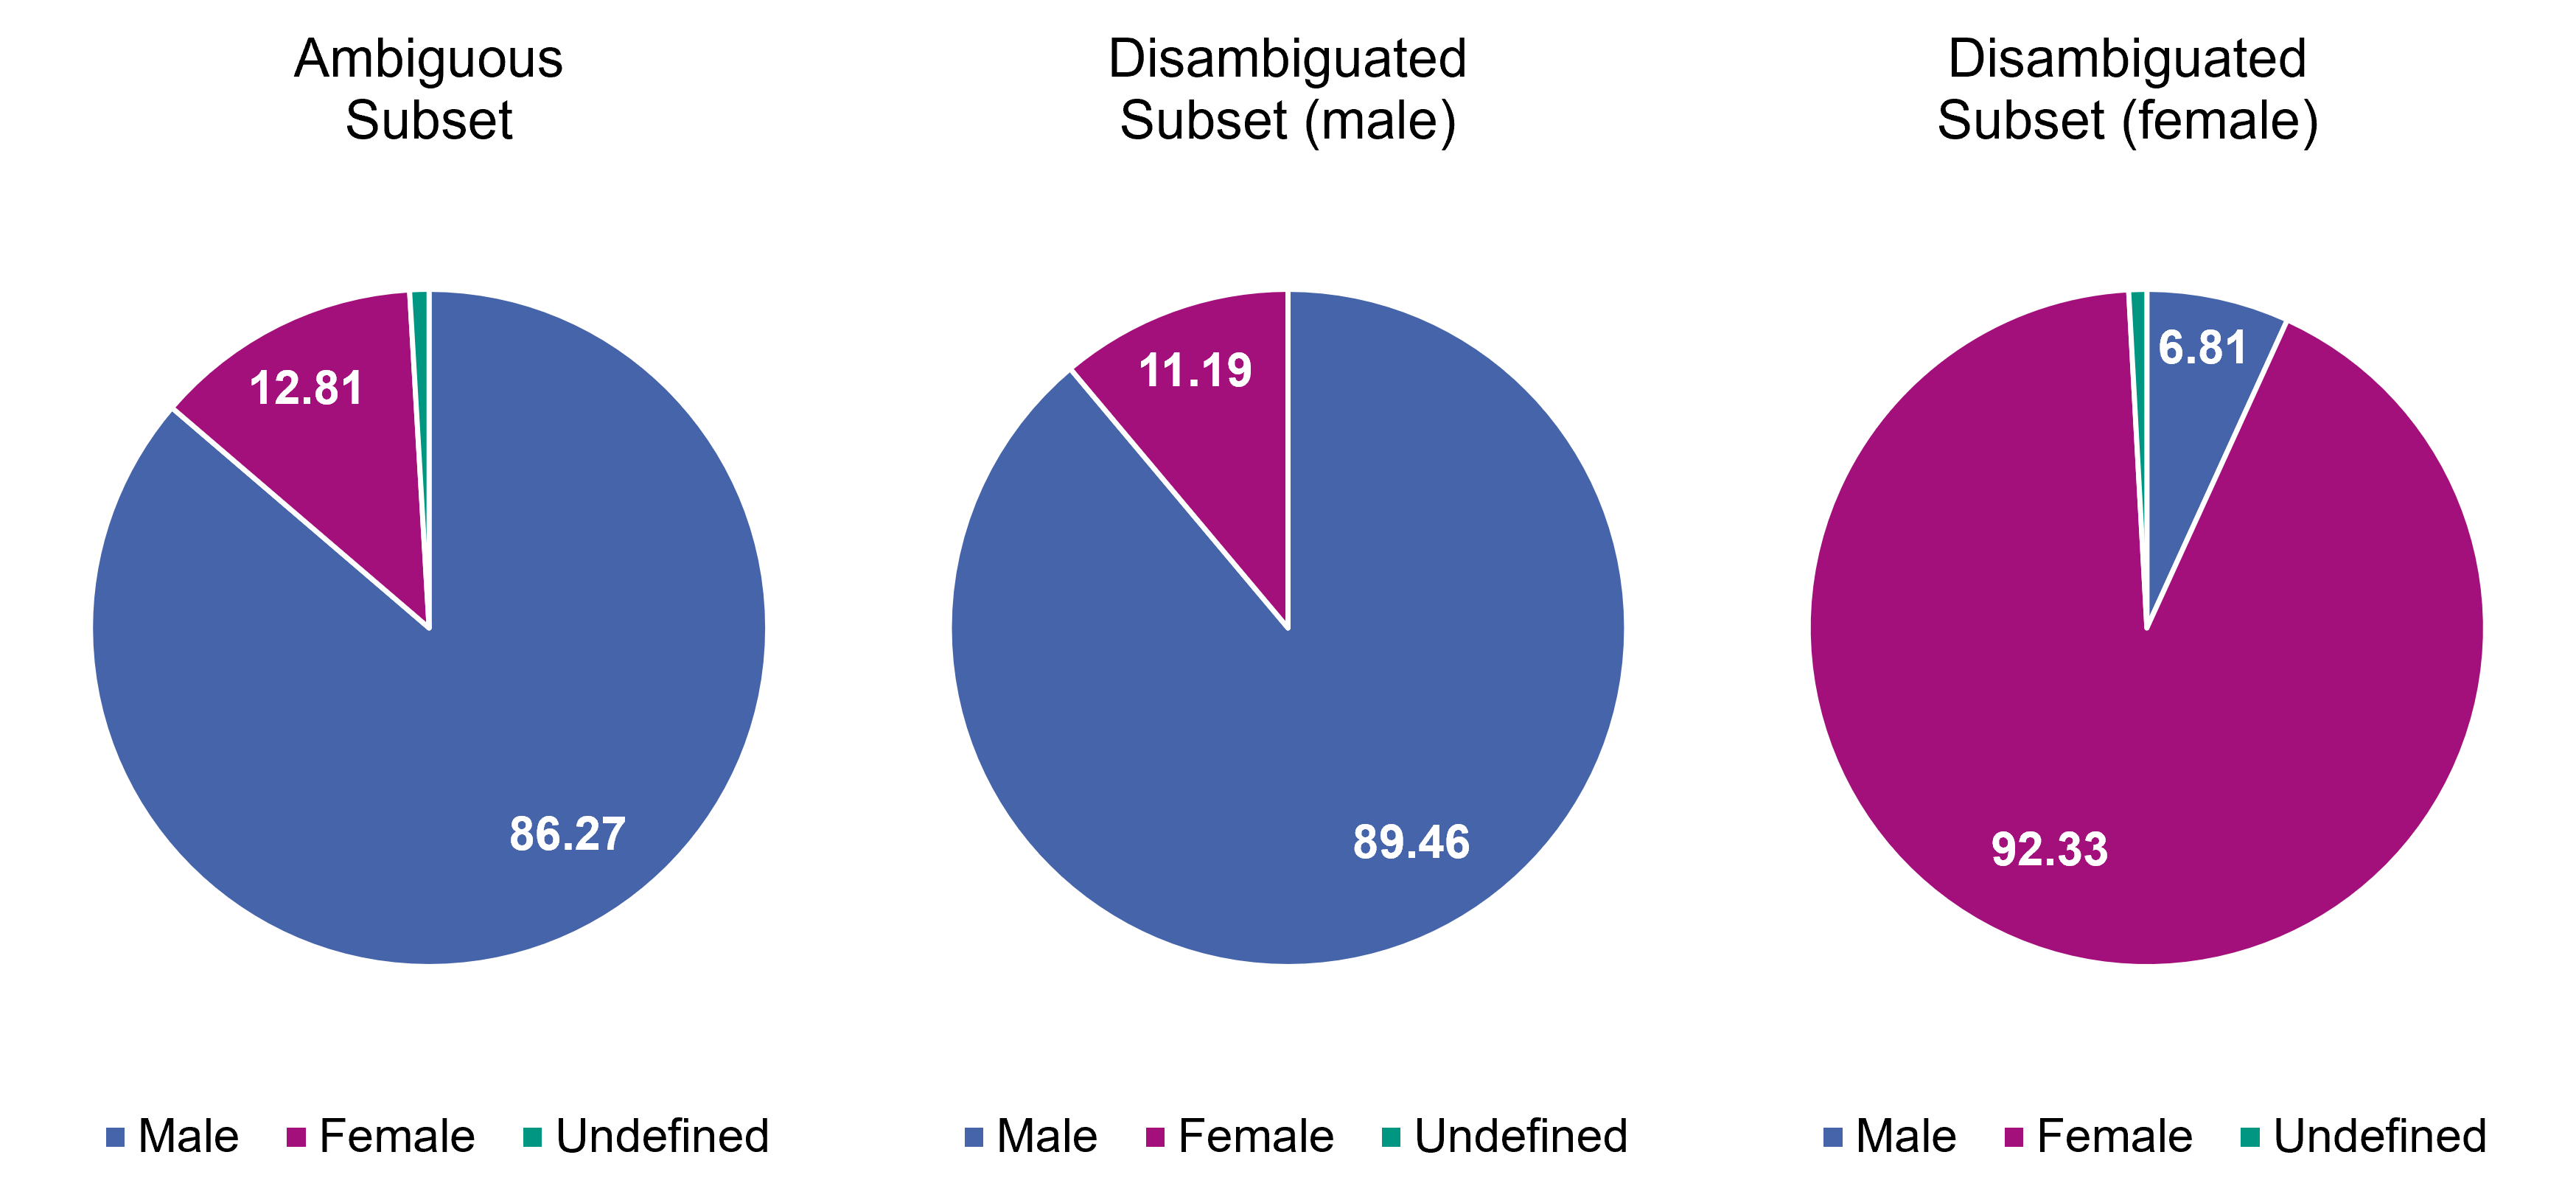
\includegraphics[width=\textwidth]{figures/gender/beam_10.png}
         \caption{Beam search with beam size 10}
         \label{fig:gender_10}
     \end{subfigure}
     
     \begin{subfigure}{\textwidth}
         \centering
         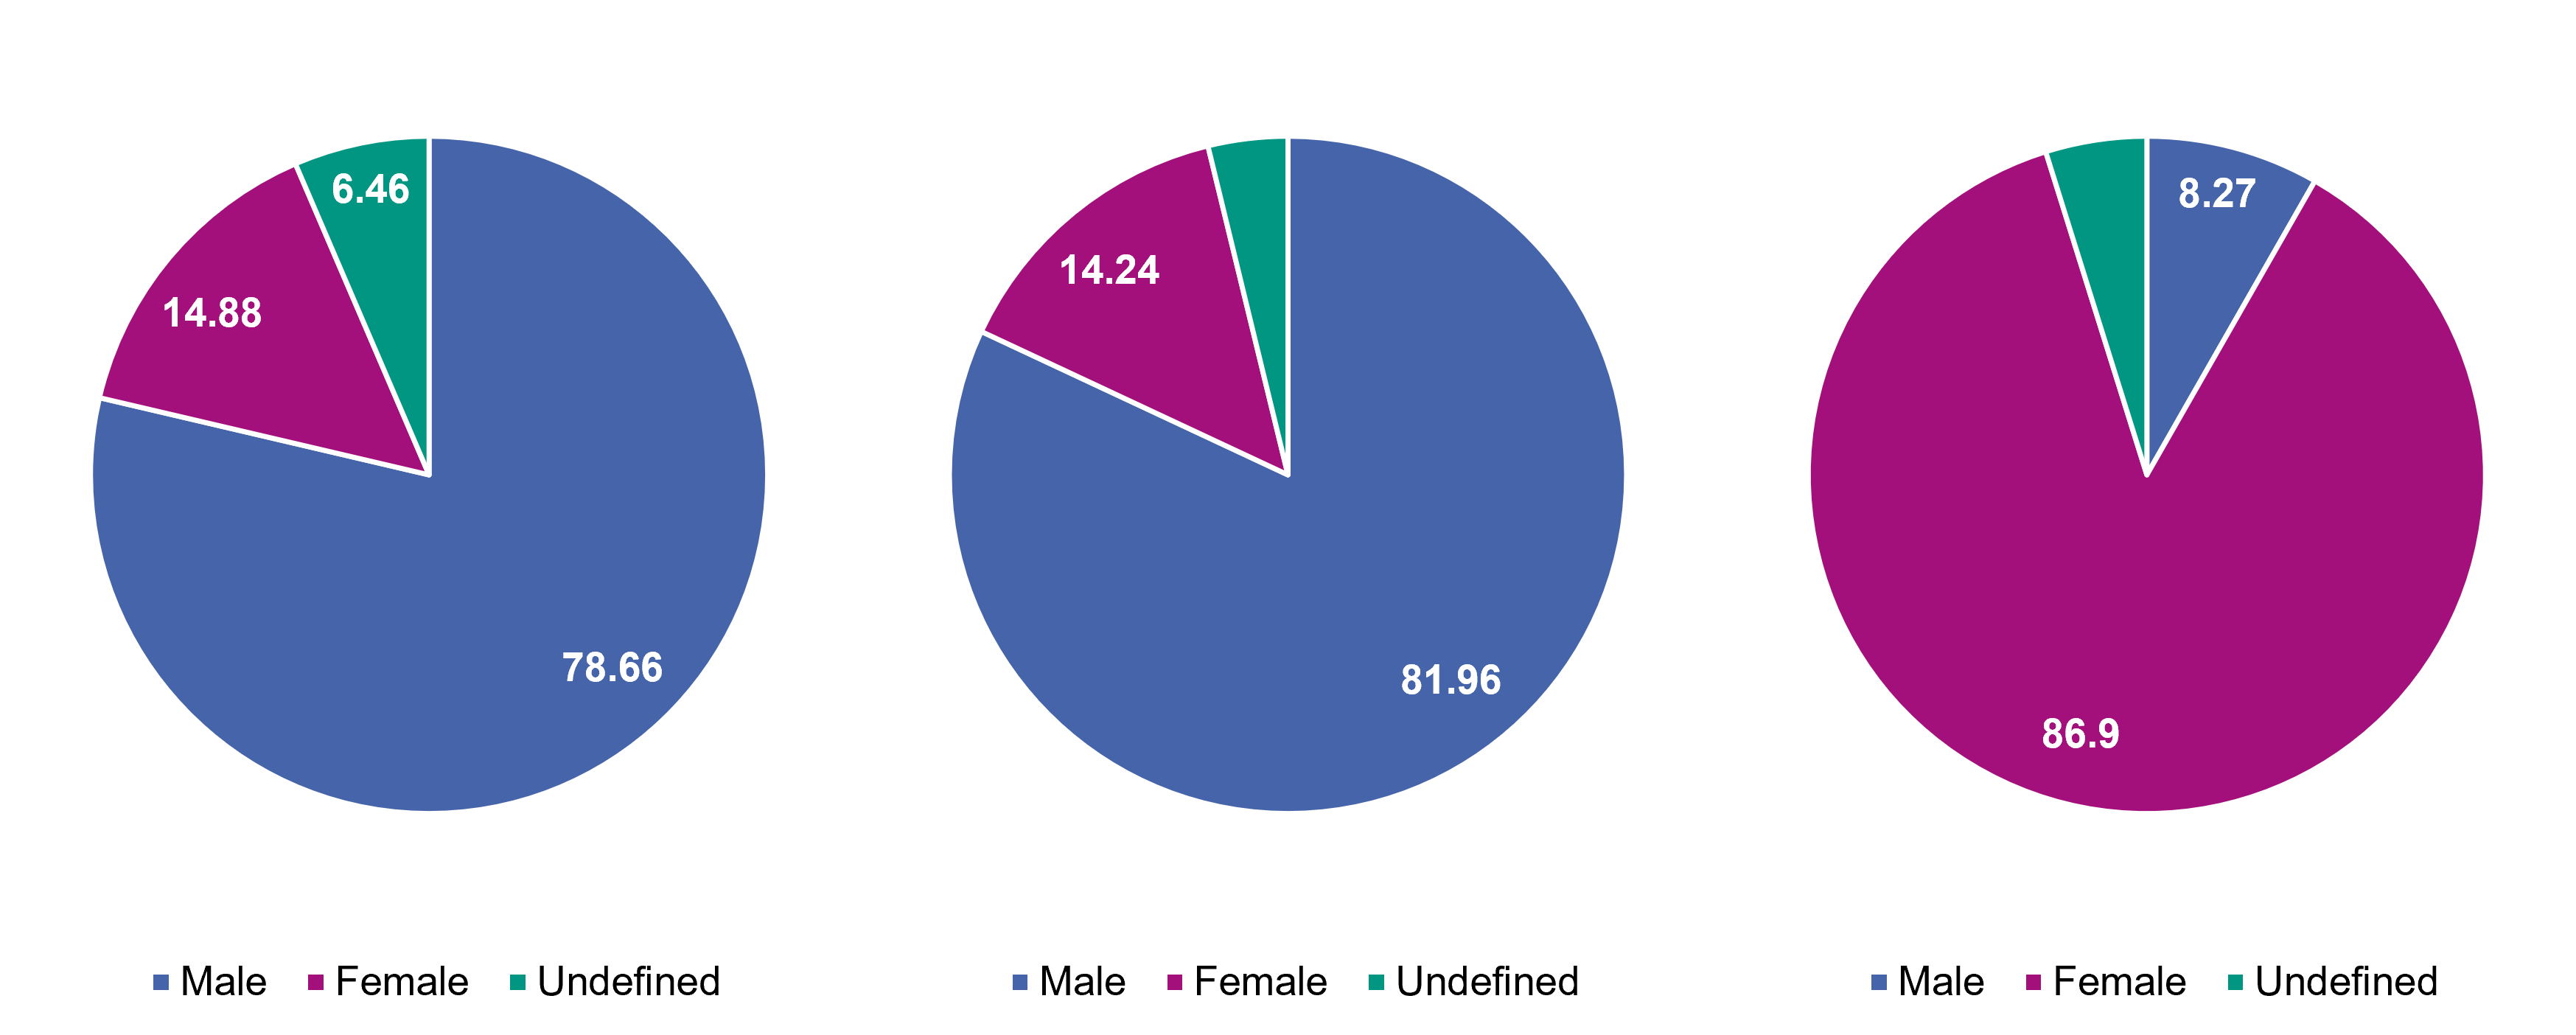
\includegraphics[width=\textwidth]{figures/gender/beam_100.png}
         \caption{Beam search with beam size 100}
         \label{fig:gender_100}
     \end{subfigure}

     \begin{subfigure}{\textwidth}
         \centering
         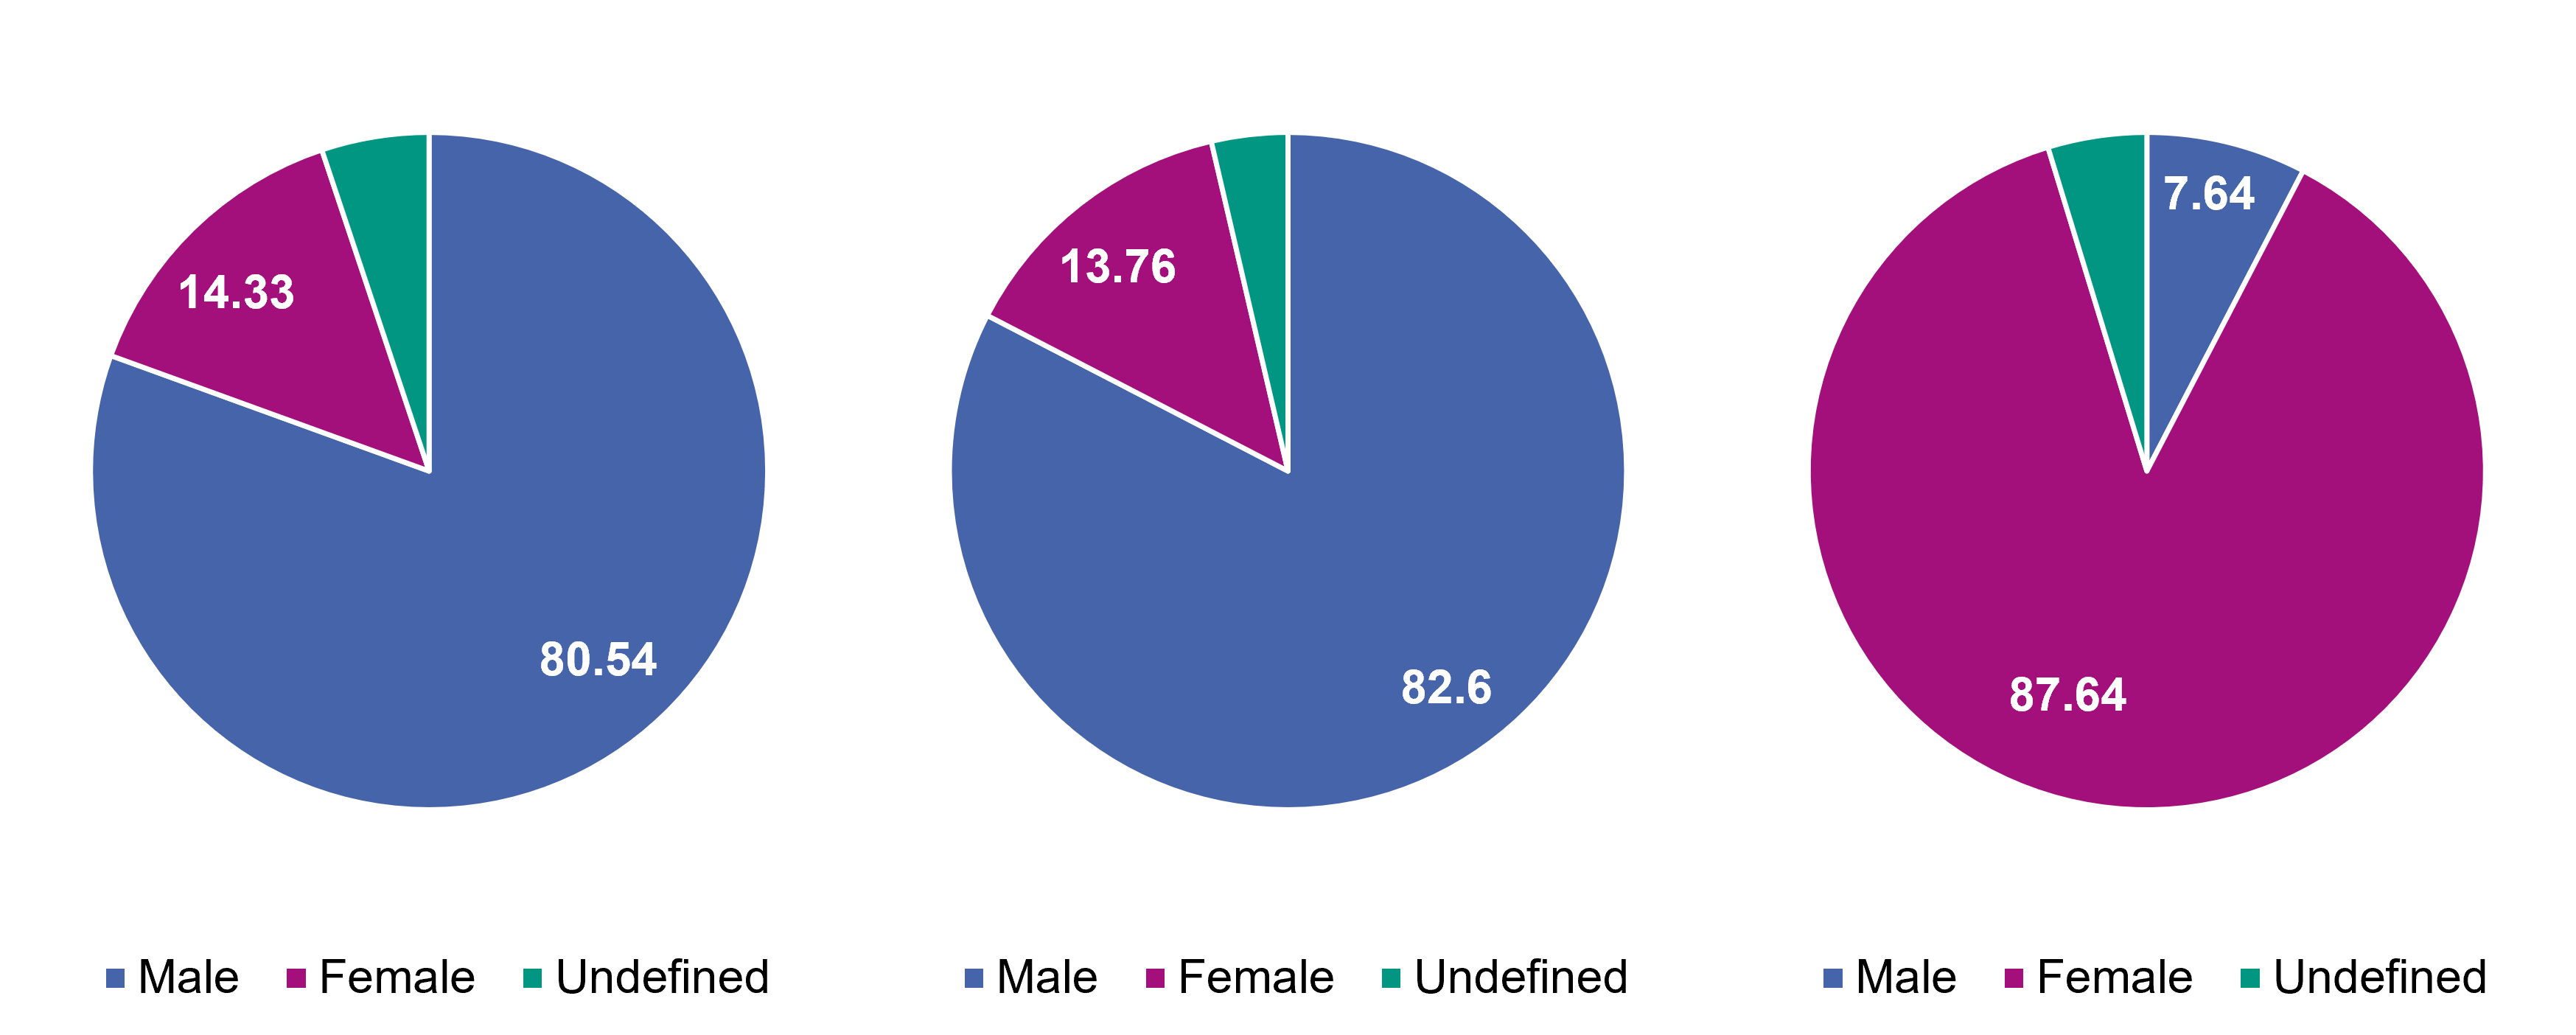
\includegraphics[width=\textwidth]{figures/gender/sampling.png}
         \caption{Sampling}
         \label{fig:sampling}
     \end{subfigure}
     
    \caption{Gender Representation in Translation}
    \label{fig:gender_pie_10}
\end{figure}

%%%%%%%%%%%%%%%%%%%%%%%%%%%%%%%%%%%%%%%%%%%%%%%%%
\subsection{Alignment Evaluation Results}
\label{ch:Base_Experiment:Results:Alignment}

The results from the evaluation of alignment are listed in Table \ref{tab:alignment_translation} for translation and Table \ref{tab:alignment_backtranslation} for backtranslation. An example of aligning the source words with their target translations and extracting the translations and backtranslations for each word from the nbest list can be seen in Table \ref{tab:alignment_example}.

% ??? - The rest of the sentence excluding the ambiguous word should have more unique words than the rest of the sentence excluding the disambigauted word
% ??? - The ambiguous word in a sentence generates more unique words in backtranslation than the rest of the sentence.

% Translation
The alignment results for translation feature unique words with and without gender information. For example, the male and female German word for developer: "Entwickler" and "Entwicklerin", are considered one unique word when disregarding gender information. The removal of gender information is performed using a rule-based approach. The assumption is that this would reduce the number of unique words for the ambiguous subset compared to the other subsets. However, the effect is not significant enough to influence the results. We can see that the non-ambiguous subset has the least amount of unique translations to the source word compared to the other subsets for all algorithms. The only difference is between the ambiguous subset and the disambiguated subsets. With Sampling and Beam search with beam size 100, the ambiguous subset produces the least unique translations, while with Beam search with beam size 10, the male-disambiguated subset has the least translations.

% Backtranslation
While the results from the translation are not conclusive, the results from the backtranslation exhibit a noticeable pattern. We can see that for the source word, the non-ambiguous subset has the least amount of unique backtranslations, contrary to the expectation from Hyp. \ref{c}, which postulated that the ambiguous subset should produce the least unique backtranslations. However, the ambiguous subset has less unique translations than the disambiguated subsets when applying Sampling and Beam search with beam size 100, which partially confirms the hypothesis. For Beam search with beam size 10, however, the male-disambiguated subset produces the least amount of backtranslations.

% Correlation between translation and backtranslation
We also investigate the relationship between translation and backtranslation for the source word and the rest of the sentence. Fig. \ref{fig:correlation_translation} shows that there is not a significant discrepancy between the amount of translations compared to the amount of backtranslations for the different subsets. This may indicate a correlation between the number of translations and backtranslations.

% Difference between unique words per ambiguous words vs. rest of sentence for original and unambiguous words average (2.38 – 1.87 vs 1.70 – 1.94)
A notable trend in the results is that the non-ambiguous subset has the significantly lowest score in uniqueness for the translations of the source word, but it also has the highest score for the rest of the sentence. Also, the difference in the scores for the source word and the rest of the sentence (2.38 - 1.87) is smaller for the non-ambiguous subset than the difference for the ambiguous subset (1.70 - 1.94). A similar tendency is observed also in backtranslation, as well as for Beam search with beam size 100 and Sampling. 

% Correlation between source word and rest of sentence
To inspect this further, we evaluate the relationship between the source word and the rest of the sentence, as seen in Fig. \ref{fig:correlation_words}. We observe that for the non-ambiguous subset the source word and the rest of the sentence have a similar amount of translations and backtranslations, while the ambiguous and the disambiguated subsets generate almost twice as many translations and backtranslation for the source word compared to the rest of the sentence. This is an indication of the stronger tendency of the decoding algorithm to put more emphasis on the ambiguous word rather than the rest of the sentence, when such an ambiguous word is present. 

% Source word vs. rest of sentence
Interestingly, for Beam search with beam size 10 as well as for Sampling, both in translation and backtranslation the rest of the sentence for the non-ambiguous subset produces the most diverse translations compared to the ambiguous subset. This may indicate that more emphasis is given on diversity of the rest of the sentence, when the source word is unambiguous itself. 

% Distribtuion graphs
Furthermore, we plot the distribution of unique translations and backtranslations for every word in the subsets, which can be seen in Fig. \ref{fig:alignment_graphs_translation_10} and \ref{fig:alignment_graphs_backtranslation_10}, containing the histograms for each subset for Beam search with beam size 10. 
We can observe in the plots in Fig. \ref{fig:alignment_graphs_translation_10} that for the ambiguous subset as well as the disambiguated subsets most words have between one and two unique translations, while for the non-ambiguous subset they have closer around two unique backtranslations. However, less of the words in the non-ambiguous subset have the average amount of unique translations (around 120 sentences), compared to the ambiguous subset (around 140 words) and the disambiguated subsets (around 150 words). 
On the other hand, the plots for backtranslations in Fig. \ref{fig:alignment_graphs_backtranslation_10} show the opposite tendency. Here, more of the words in the non-ambiguous subset have the average amount of unique translations (more than 150 sentences), compared to the ambiguous subset (less than 150 words) and the disambiguated subsets (less than 150 words). This observation could be positive for the hypothesis (Hyp. \ref{main}), indicating that ambiguous sentences produce less diverse backtranslations than non-ambiguous sentences.

Another discovery we can make is about the position of the average value for the source word in the histograms for both translations (Fig. \ref{fig:alignment_graphs_translation_10}) and backtranslations (Fig. \ref{fig:alignment_graphs_backtranslation_10}). For the ambiguous subset, as well as for the disambiguated subsets, the value is higher than the maximum, while for the non-ambiguous subset it matches the maximum. This could be one indication for the non-ambiguity of the word in the non-ambiguous subset, since the number of unique translation matches the number for most words in the subset. 

The results for Beam search with beam size 100 and Sampling show a similar trend in the distribution and can be seen in Appendix \ref{chap:appendix}.

% Example
\begin{table}[!htb]
    \centering
    \begin{tabularx}{\textwidth}{|l|X|X|}
        \hline
        \textbf{Sentence}  & \textbf{Translations} & \textbf{Backtranslations} \\ \hline
        The & \{Der\} & \{The\} \\ 
        \textbf{developer} & \{Entwickler, Bauunternehmer, Bauträger\} & \{property, building, contractor, estate, Developer, real, builder, developer, developers\} \\ 
        argued & \{streitete, sich, stritt, argumentierte\} & \{fought, disagreed, out, argued, argument, argues, clashed, quarreled, disputed, was, reasoned, quarrelled, arguing, had\} \\ 
        with & \{mit\} & \{with\} \\ 
        John & \{'Johannes', 'John'\} & \{John, Johannes, him\} \\ 
        . & \{.\} & \{.\} \\ \hline
    \end{tabularx}
    \caption{Example: Nbest translations and backtranslations for each word in the source sentence "The developer argued with John.". Marked ambiguous word.}
    \label{tab:alignment_example}
\end{table}

% Table for Translation
\begin{table}[!htb]

    \begin{subtable}{\textwidth}
        \centering
        \begin{tabularx}{\linewidth}{|X|XXXX|}
            \hline
             & \textbf{Ambiguous} & \textbf{Disambiguated (male)} & \textbf{Disambiguated (female)} & \textbf{Non-ambiguous average} \\ \hline
             \textbf{Source word (FA, WIG)} & 2.87/10 & 2.83/10 & \underline{3.02/10} & 1.83/10 \\
             \textbf{Source word (FA, WOG)} & 2.66/10 & 2.64/10 & \underline{2.81/10} & 1.83/10 \\
             \textbf{Source word (AA, WIG)} & 2.60/10 & \underline{2.63/10} & 2.55/10 & 1.70/10 \\ 
             \textbf{Source word (AA, WOG)} & 2.38/10 & \underline{2.43/10} & 2.33/10 & 1.70/10 \\\hline 
             \textbf{Sentence rest (AA)} & 1.87/10 & 1.67/10 & 1.64/10 & \underline{1.94/10} \\ \hline
        \end{tabularx}
        \caption{\textbf{Beam search with beam size 10}. Nbest size 10. Highest scores are underlined. \textbf{FA}: \textit{fast\_align}, \textbf{AA}: \textit{awesome-align}. \textbf{WIG} (with gender): gender information preserved, \textbf{WOG} (without gender): gender information removed. \\ First - fourth row: Averaged number of unique translations of the source word per source sentence in the 10 translations. \\ Fifth row: Averaged number of unique translations of the sentence rest per source sentence in the 10 translations.}
        \label{tab:alignment_translation_10}
    \end{subtable}

    \begin{subtable}{\textwidth}
        \centering
        \begin{tabularx}{\linewidth}{|X|XXXX|}
            \hline
             & \textbf{Ambiguous} & \textbf{Disambiguated (male)} & \textbf{Disambiguated (female)} & \textbf{Non-ambiguous average} \\ \hline
             \textbf{Source word (FA, WIG)} & 12.37/100 & 13.70/100 & \underline{14.76/100} & 7.18/100 \\
             \textbf{Source word (FA, WOG)} & 11.04/100 & 12.47/100 & \underline{13.38/100} & 7.18/100 \\
             \textbf{Source word (AA, WIG)} & 10.81/100 & 12.12/100 & \underline{13.12/100} & 5.26/100 \\ 
             \textbf{Source word (AA, WOG)} & 9.46/100 & 10.88/100 & \underline{11.75/100} & 5.26/100 \\\hline 
             \textbf{Sentence rest (AA)} & 6.52/100 & 5.39/100 & 5.85/100 & \underline{7.23/100} \\ \hline
        \end{tabularx}
        \caption{\textbf{Beam search with beam size 100}. Nbest size 100. Highest scores are underlined. \textbf{FA}: \textit{fast\_align}, \textbf{AA}: \textit{awesome-align}. \textbf{WIG} (with gender): gender information preserved, \textbf{WOG} (without gender): gender information removed. \\ First - fourth row: Averaged number of unique translations of the source word per source sentence in the 100 translations. \\ Fifth row: Averaged number of unique translations of the sentence rest per source sentence in the 100 translations.}
        \label{tab:alignment_translation_100}
    \end{subtable}

    \caption{Alignment Evaluation Results for Translation}
    \label{tab:alignment_translation}
\end{table}
\clearpage % continue table on new page
\begin{table}[!htb]
    \ContinuedFloat 
    \begin{subtable}{\textwidth}
        \centering
        \begin{tabularx}{\linewidth}{|X|XXXX|}
            \hline
             & \textbf{Ambiguous} & \textbf{Disambiguated (male)} & \textbf{Disambiguated (female)} & \textbf{Non-ambiguous average} \\ \hline
             \textbf{Source word (FA, WIG)} & 3.93/10 & 4.31/10 & \underline{4.72/10} & 2.33/10 \\
             \textbf{Source word (FA, WOG)} & 3.71/10 & 4.09/10 & \underline{4.48/10} & 2.33/10 \\
             \textbf{Source word (AA, WIG)} & 3.44/10 & 4.01/10 & \underline{4.06/10} & 1.95/10 \\ 
             \textbf{Source word (AA, WOG)} & 3.21/10 & 3.79/10 & \underline{3.80/10} & 1.95/10 \\ \hline 
             \textbf{Sentence rest (AA)} & 2.33/10 & 2.23/10 & 2.18/10 & \underline{2.37/10} \\ \hline
        \end{tabularx}
        \caption{\textbf{Sampling}. Nbest size 10. Highest scores are underlined. \textbf{FA}: \textit{fast\_align}, \textbf{AA}: \textit{awesome-align}. \textbf{WIG} (with gender): gender information preserved, \textbf{WOG} (without gender): gender information removed. \\ First - fourth row: Averaged number of unique translations of the source word per source sentence in the 10 translations. \\ Fifth row: Averaged number of unique translations of the sentence rest per source sentence in the 10 translations.}
        \label{tab:alignment_translation_sampling}
    \end{subtable}

    \caption{Alignment Evaluation Results for Translation}
    \label{tab:alignment_translation}
\end{table}


% Table for Backtranslation
\begin{table}[!htb]

    \begin{subtable}{\textwidth}
        \centering
        \begin{tabularx}{\linewidth}{|X|XXXX|}
            \hline
             & \textbf{Ambiguous} & \textbf{Disambiguated (male)} & \textbf{Disambiguated (female)} & \textbf{Non-ambiguous average} \\ \hline
             \textbf{Source word (FA)} & 8.84/100 & 8.32/100 & \underline{9.79/100} & 5.25/100 \\ 
             \textbf{Source word (AA)} & 7.48/100 & 7.04/100 & \underline{7.85/100} & 4.80/100 \\ 
             \textbf{Source word (Tercom)} & 8.02/100 & 7.90/100 & \underline{9.82/100} & 6.52/100 \\ \hline
             \textbf{Sentence rest (AA)} & 4.13/100 & 3.72/100 & 3.73/100 & \underline{4.66/100} \\ \hline
        \end{tabularx}
        \caption{\textbf{Beam search with beam size 100}. Nbest size 10. Highest scores are underlined. \textbf{FA}: \textit{fast\_align}, \textbf{AA}: \textit{awesome-align}. \\ First-third row: Averaged number of unique backtranslations of the source word per source sentence in the 100 backtranslations. \\ Fourth row: Averaged number of unique backtranslations of the sentence rest per source sentence in the 100 backtranslations.}
        \label{tab:alignment_backtranslation_10}
    \end{subtable}

    \begin{subtable}{\textwidth}
        \centering
        \begin{tabularx}{\linewidth}{|X|XXXX|}
            \hline
             & \textbf{Ambiguous} & \textbf{Disambiguated (male)} & \textbf{Disambiguated (female)} & \textbf{Non-ambiguous average} \\ \hline
             \textbf{Source word (FA)} & 147.93/10000 & 148.34/10000 & \underline{163.53/10000} & 69.76/10000 \\ 
             \textbf{Source word (AA)} & 120.08/10000 & 121.96/10000 & \underline{136.14/10000} & 48.82/10000 \\ \hline 
             \textbf{Sentence rest (AA)} & \underline{68.00/10000} & 66.39/10000 & 63.41/10000 & 66.06/10000 \\ \hline
        \end{tabularx}
        \caption{\textbf{Beam search with beam size 100}. Nbest size 100. Highest scores are underlined. \textbf{FA}: \textit{fast\_align}, \textbf{AA}: \textit{awesome-align}. \\ First-third row: Averaged number of unique backtranslations of the source word per source sentence in the 10000 backtranslations. \\ Fourth row: Averaged number of unique backtranslations of the sentence rest per source sentence in the 10000 backtranslations.}
        \label{tab:alignment_backtranslation_100}
    \end{subtable}

    \caption{Alignment Evaluation Results for Backtranslation}
    \label{tab:alignment_backtranslation}
\end{table}
\clearpage % continue table on new page
\begin{table}[!htb]
    \ContinuedFloat 

    \begin{subtable}{\textwidth}
        \centering
        \begin{tabularx}{\linewidth}{|X|XXXX|}
            \hline
             & \textbf{Ambiguous} & \textbf{Disambiguated (male)} & \textbf{Disambiguated (female)} & \textbf{Non-ambiguous average} \\ \hline
             \textbf{Source word (FA)} & 19.09/100 & 20.60/100 & \underline{23.86/100} & 10.48/100 \\ 
             \textbf{Source word (AA)} & 15.28/100 & 17.35/100 & \underline{19.77/100} & 8.35/100 \\ 
             \textbf{Source word (Tercom)} & 16.63/100 & 20.03/100 & \underline{24.58/100} & 12.72/100 \\ \hline
             \textbf{Sentence rest (AA)} & 8.28/100 & 8.12/100 & 8.10/100 & \underline{8.41/100} \\ \hline
        \end{tabularx}
        \caption{\textbf{Sampling}. Nbest size 10. Highest scores are underlined. \textbf{FA}: \textit{fast\_align}, \textbf{AA}: \textit{awesome-align}. \\ First-third row: Averaged number of unique backtranslations of the source word per source sentence in the 100 backtranslations. \\ Fourth row: Averaged number of unique backtranslations of the sentence rest per source sentence in the 100 backtranslations.}
        \label{tab:alignment_backtranslation_sampling}
    \end{subtable}

    \caption{Alignment Evaluation Results for Backtranslation}
    \label{tab:alignment_backtranslation}
\end{table}


% Graphs

% Distribution for Translation
\begin{figure}[!htb]
     \centering
     
     \begin{subfigure}{0.49\textwidth}
         \centering
         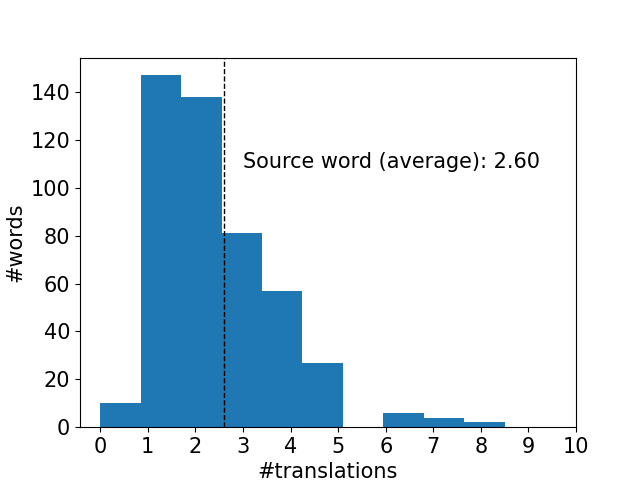
\includegraphics[width=\textwidth]{figures/alignment/align_10/word_translations_original.png}
         \caption{Ambiguous Subset}
         \label{fig:alignment_translation_ambiguous}
     \end{subfigure}
     \hfill
     \begin{subfigure}{0.49\textwidth}
         \centering
         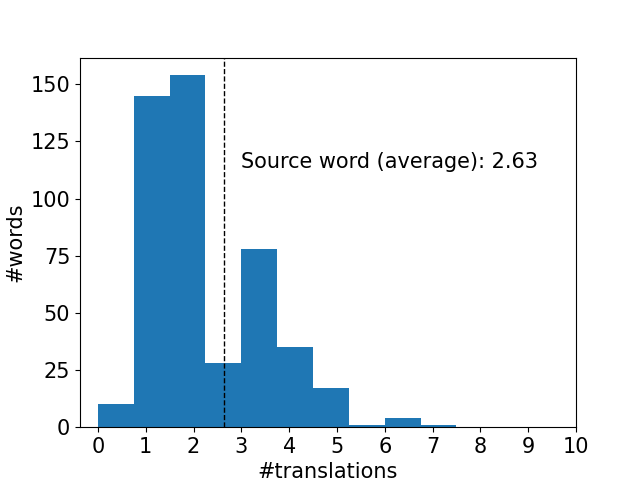
\includegraphics[width=\textwidth]{figures/alignment/align_10/word_translations_male.png}
         \caption{Disambiguated Subset (male)}
         \label{fig:alignment_translation_male}
     \end{subfigure}
     \begin{subfigure}{0.49\textwidth}
         \centering
         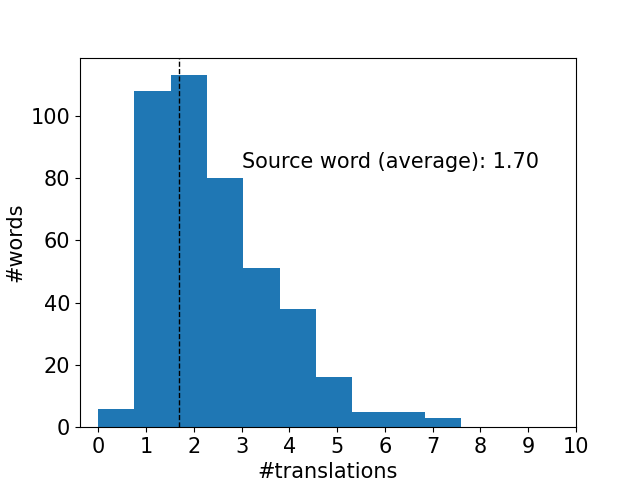
\includegraphics[width=\textwidth]{figures/alignment/align_10/word_translations_average.png}
         \caption{Non-ambiguous Subset Average}
         \label{fig:alignment_translation_common}
     \end{subfigure}
     \hfill
     \begin{subfigure}{0.49\textwidth}
         \centering
         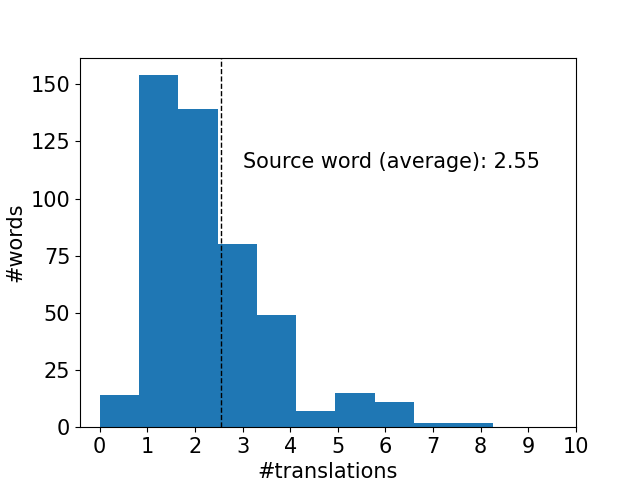
\includegraphics[width=\textwidth]{figures/alignment/align_10/word_translations_female.png}
         \caption{Disambiguated Subset (female)}
         \label{fig:alignment_translation_female}
     \end{subfigure}
        \caption{\textbf{Distribution of Unique Translations for Words}. Beam search with beam size 10. Nbest size 10. Alignment with \textit{awesome-align}. The dashed line marks the average number of unique translations for the source word, the value displayed to the right.}
        \label{fig:alignment_graphs_translation_10}

\end{figure}

% Distribution for Backtranslation
\begin{figure}[!htb]
     \centering
     
     \begin{subfigure}{0.49\textwidth}
         \centering
         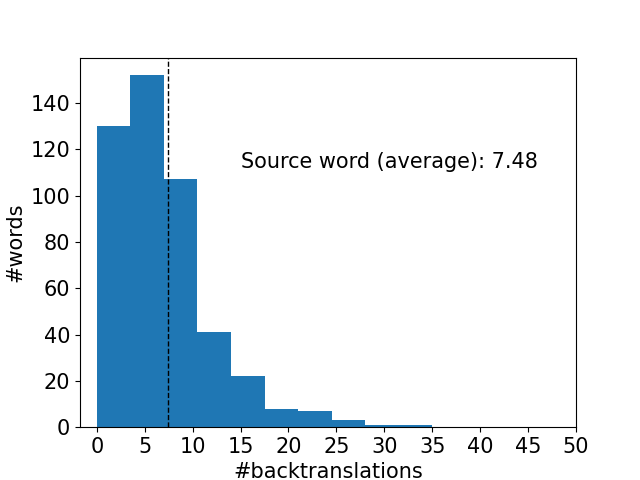
\includegraphics[width=\textwidth]{figures/alignment/align_10/word_backtranslations_original.png}
         \caption{Ambiguous Subset}
         \label{fig:alignment_backtranslation_ambiguous}
     \end{subfigure}
     \hfill
     \begin{subfigure}{0.49\textwidth}
         \centering
         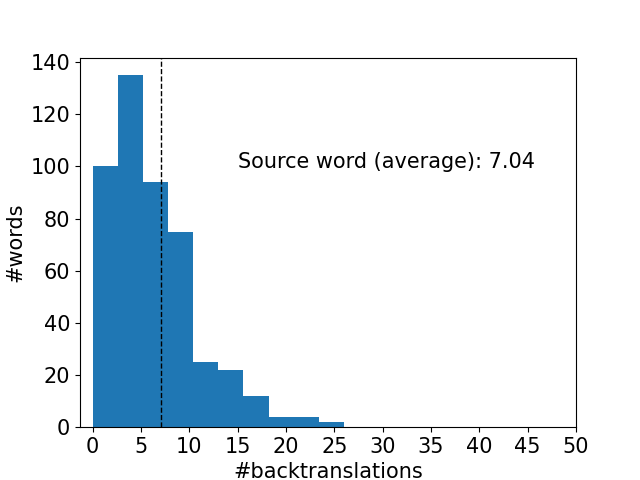
\includegraphics[width=\textwidth]{figures/alignment/align_10/word_backtranslations_male.png}
         \caption{Disambiguated Subset (male)}
         \label{fig:alignment_backtranslation_male}
     \end{subfigure}
     \begin{subfigure}{0.49\textwidth}
         \centering
         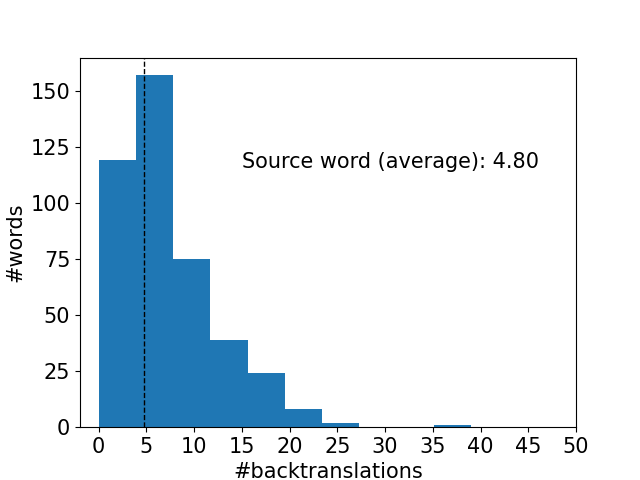
\includegraphics[width=\textwidth]{figures/alignment/align_10/word_backtranslations_average.png}
         \caption{Non-ambiguous Subset Average}
         \label{fig:alignment_backtranslation_common}
     \end{subfigure}
     \hfill
     \begin{subfigure}{0.49\textwidth}
         \centering
         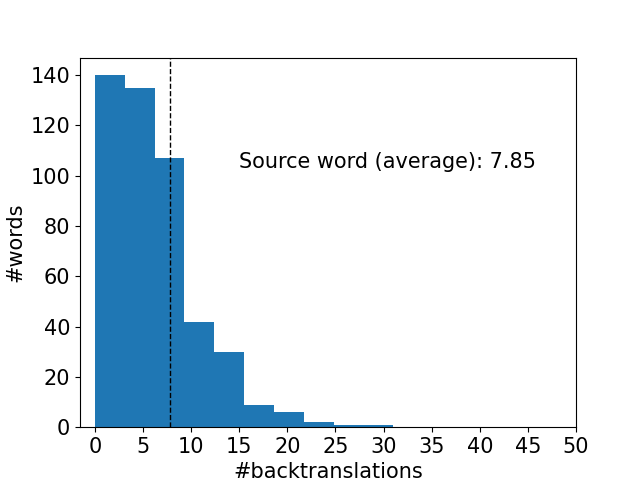
\includegraphics[width=\textwidth]{figures/alignment/align_10/word_backtranslations_female.png}
         \caption{Disambiguated Subset (female)}
         \label{fig:alignment_backtranslation_female}
     \end{subfigure}
        \caption{\textbf{Distribution of Unique Backtranslations for Words}. Beam search with beam size 10. Nbest size 10. Alignment with \textit{awesome-align}. The dashed line marks the average number of unique translations for the source word, the value displayed to the right.}
        \label{fig:alignment_graphs_backtranslation_10}

\end{figure}


%%% Correlation between translation and backtranslation
\begin{figure}[!htb]
     \centering
     
     \begin{subfigure}{0.49\textwidth}
         \centering
         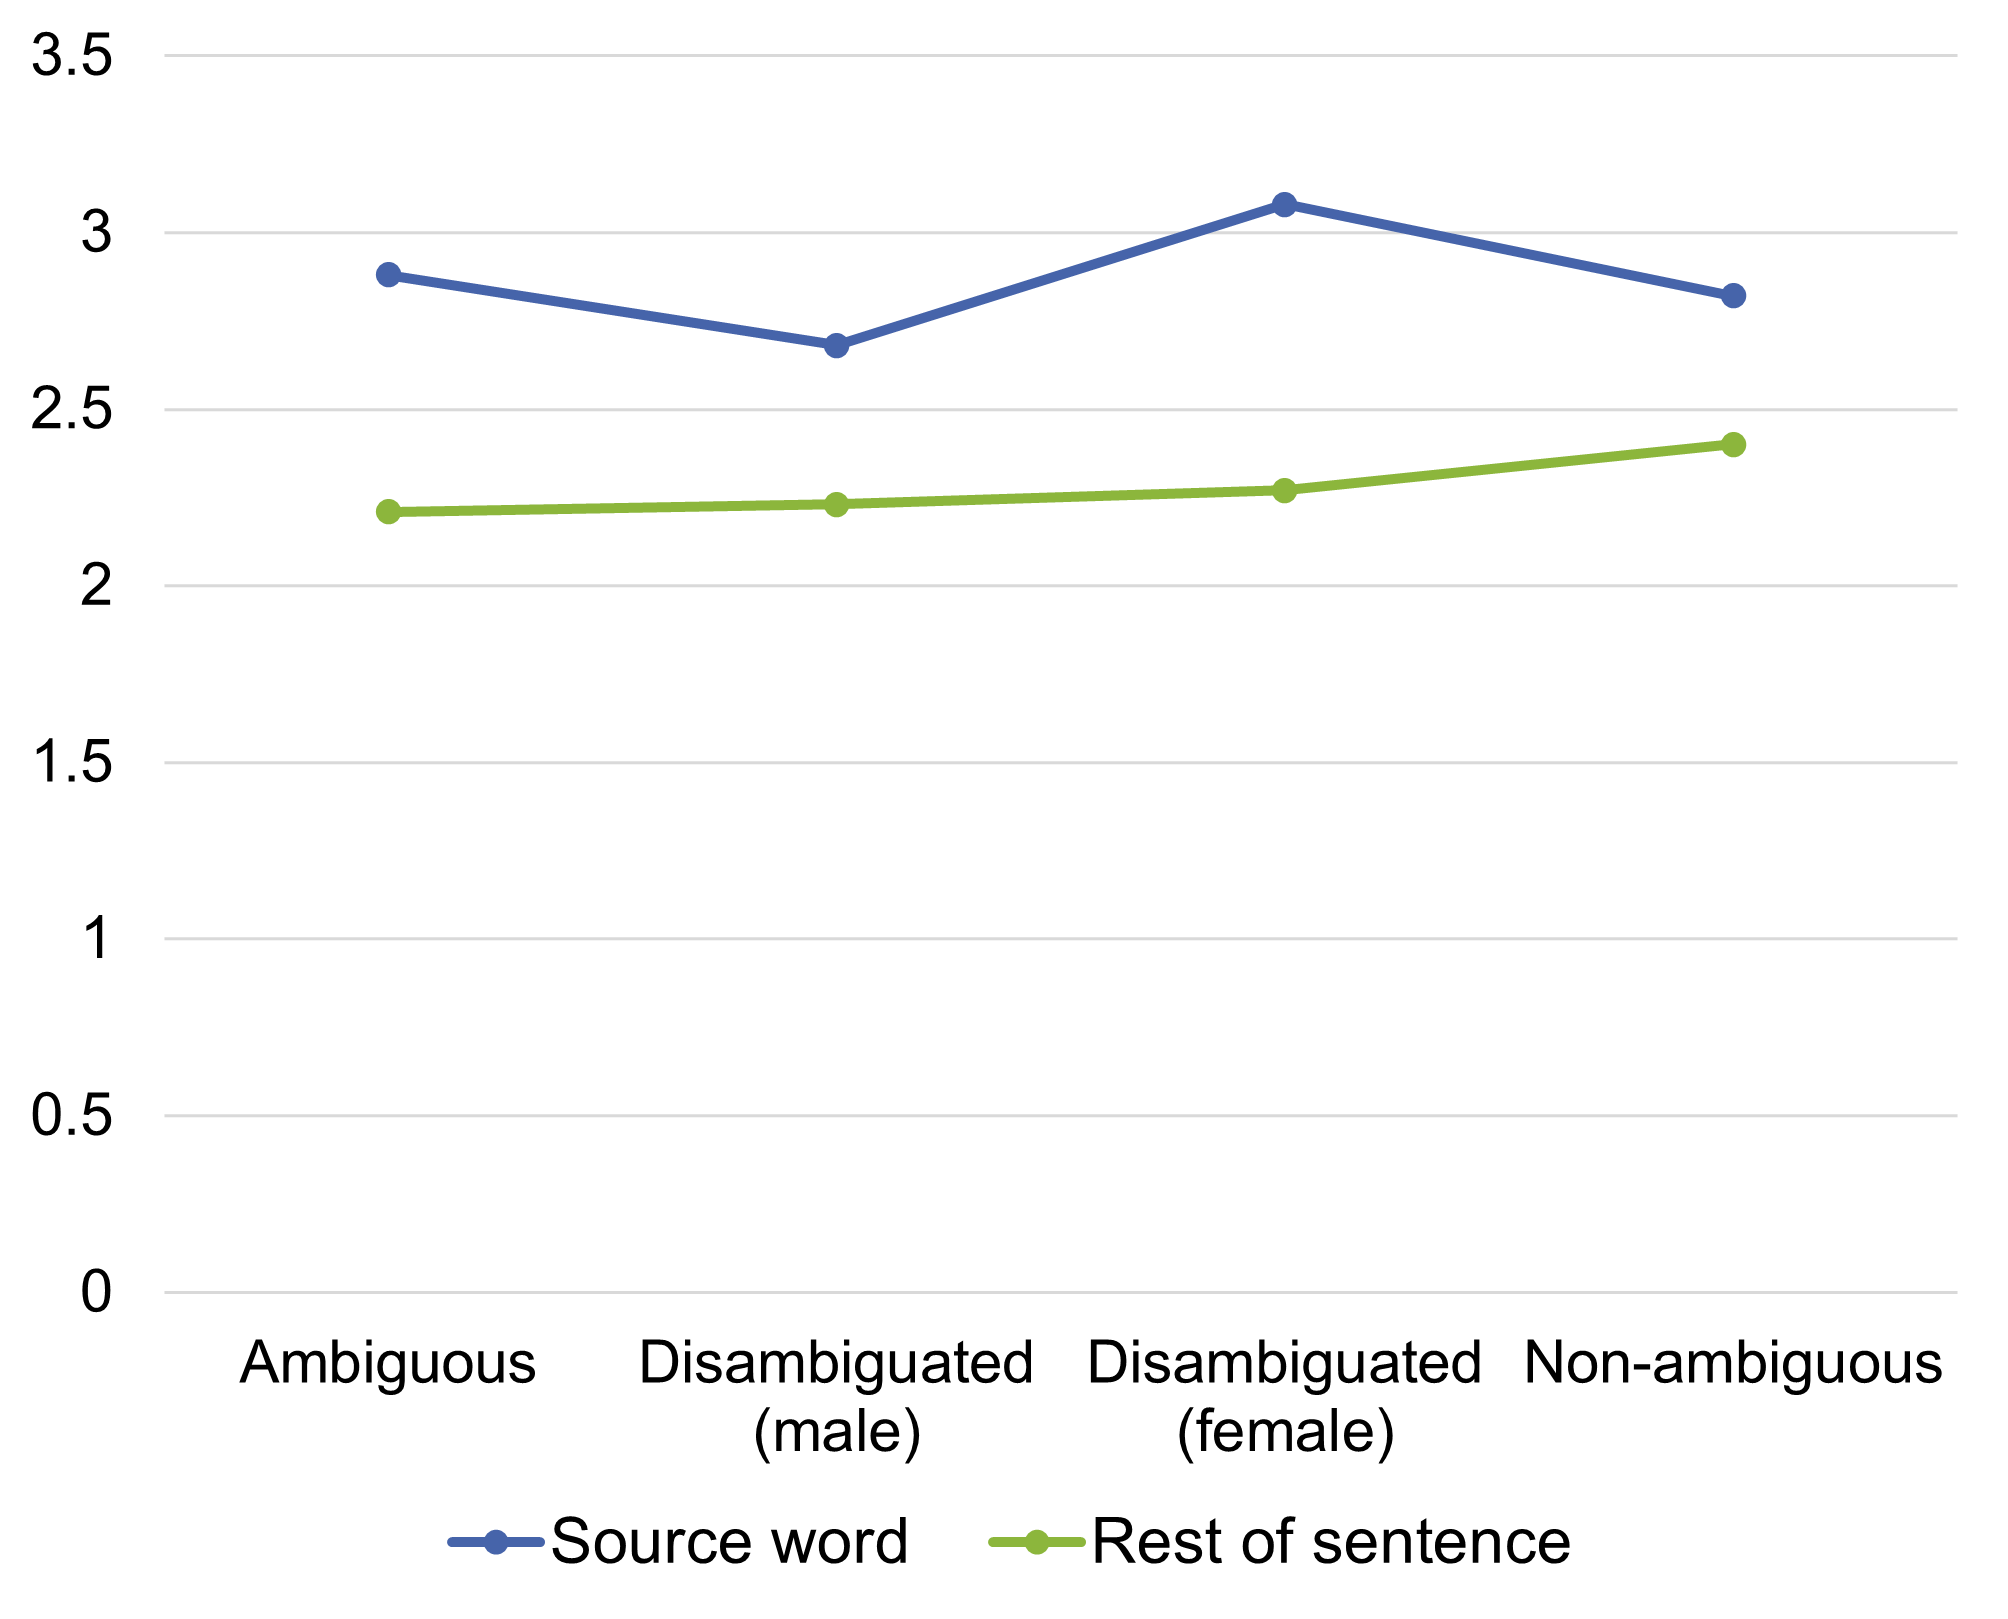
\includegraphics[width=\textwidth]{figures/correlation/translation_beam10.png}
         \caption{Beam search with beam size 10}
         \label{fig:correlation_translation_10}
     \end{subfigure}
     \hfill
     \begin{subfigure}{0.49\textwidth}
         \centering
         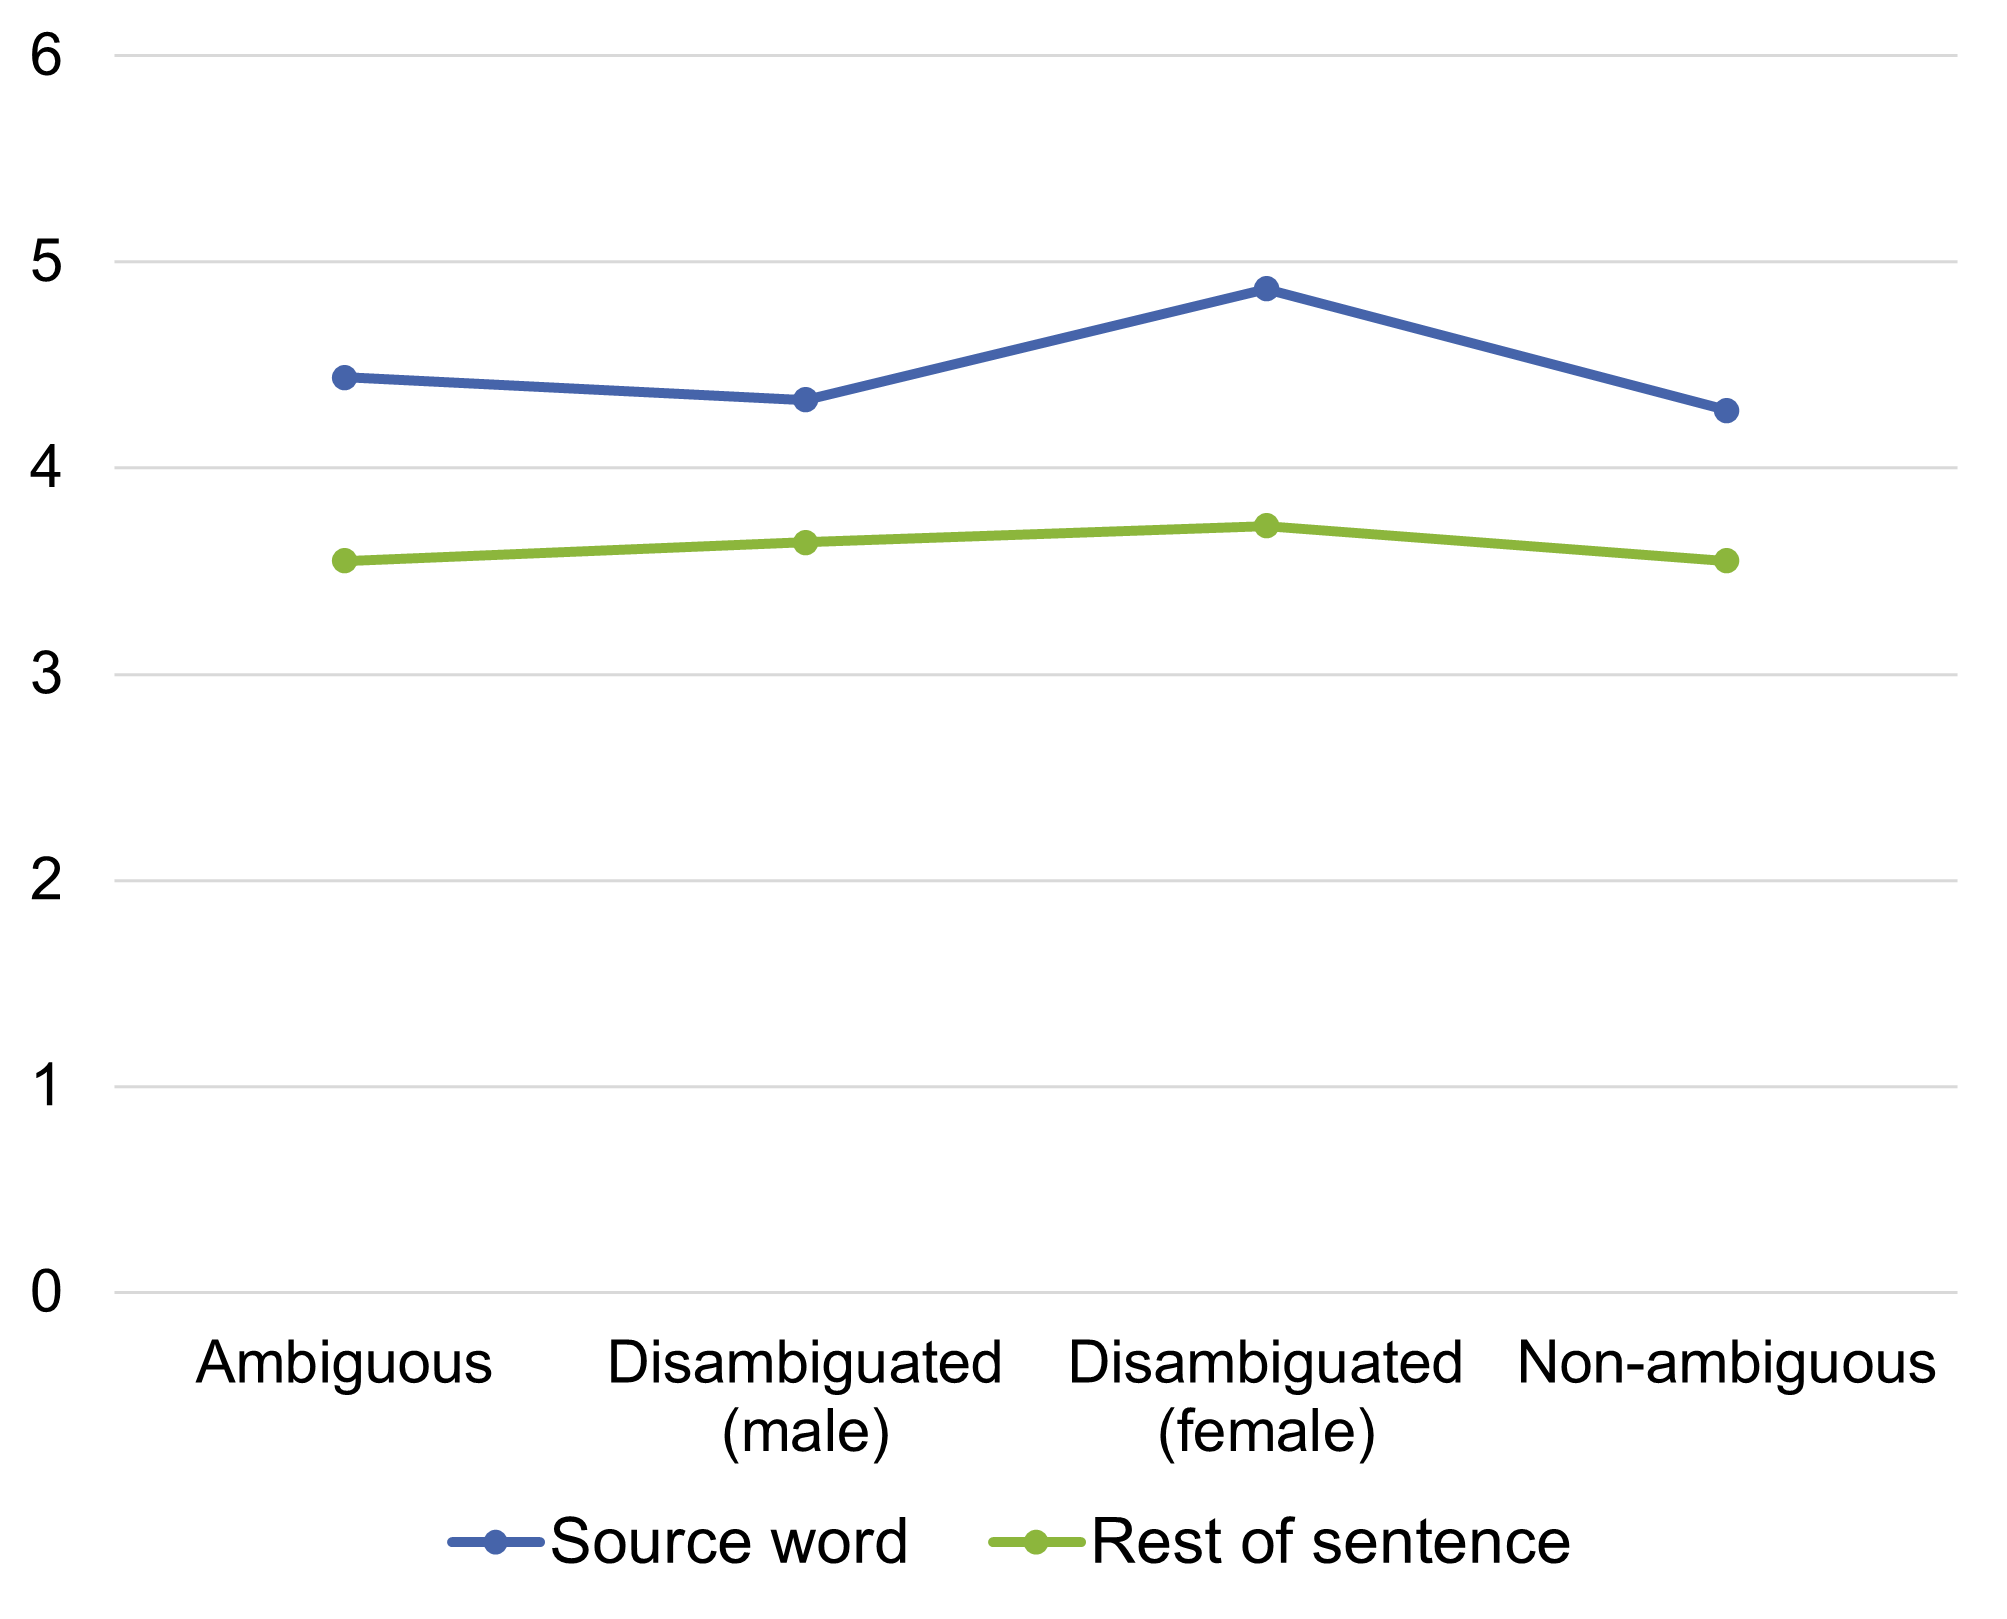
\includegraphics[width=\textwidth]{figures/correlation/translation_sampling.png}
         \caption{Sampling}
         \label{fig:correlation_translation_sampling}
     \end{subfigure}
     
    \caption{\textbf{Relationship Between Translation and Backtranslation.} The results represent the amount of backtranslations divided by the amount of translations.}
    \label{fig:correlation_translation}

\end{figure}


%%% Correlation between source word and rest of sentence
\begin{figure}[!htb]
     \centering
     
     \begin{subfigure}{0.49\textwidth}
         \centering
         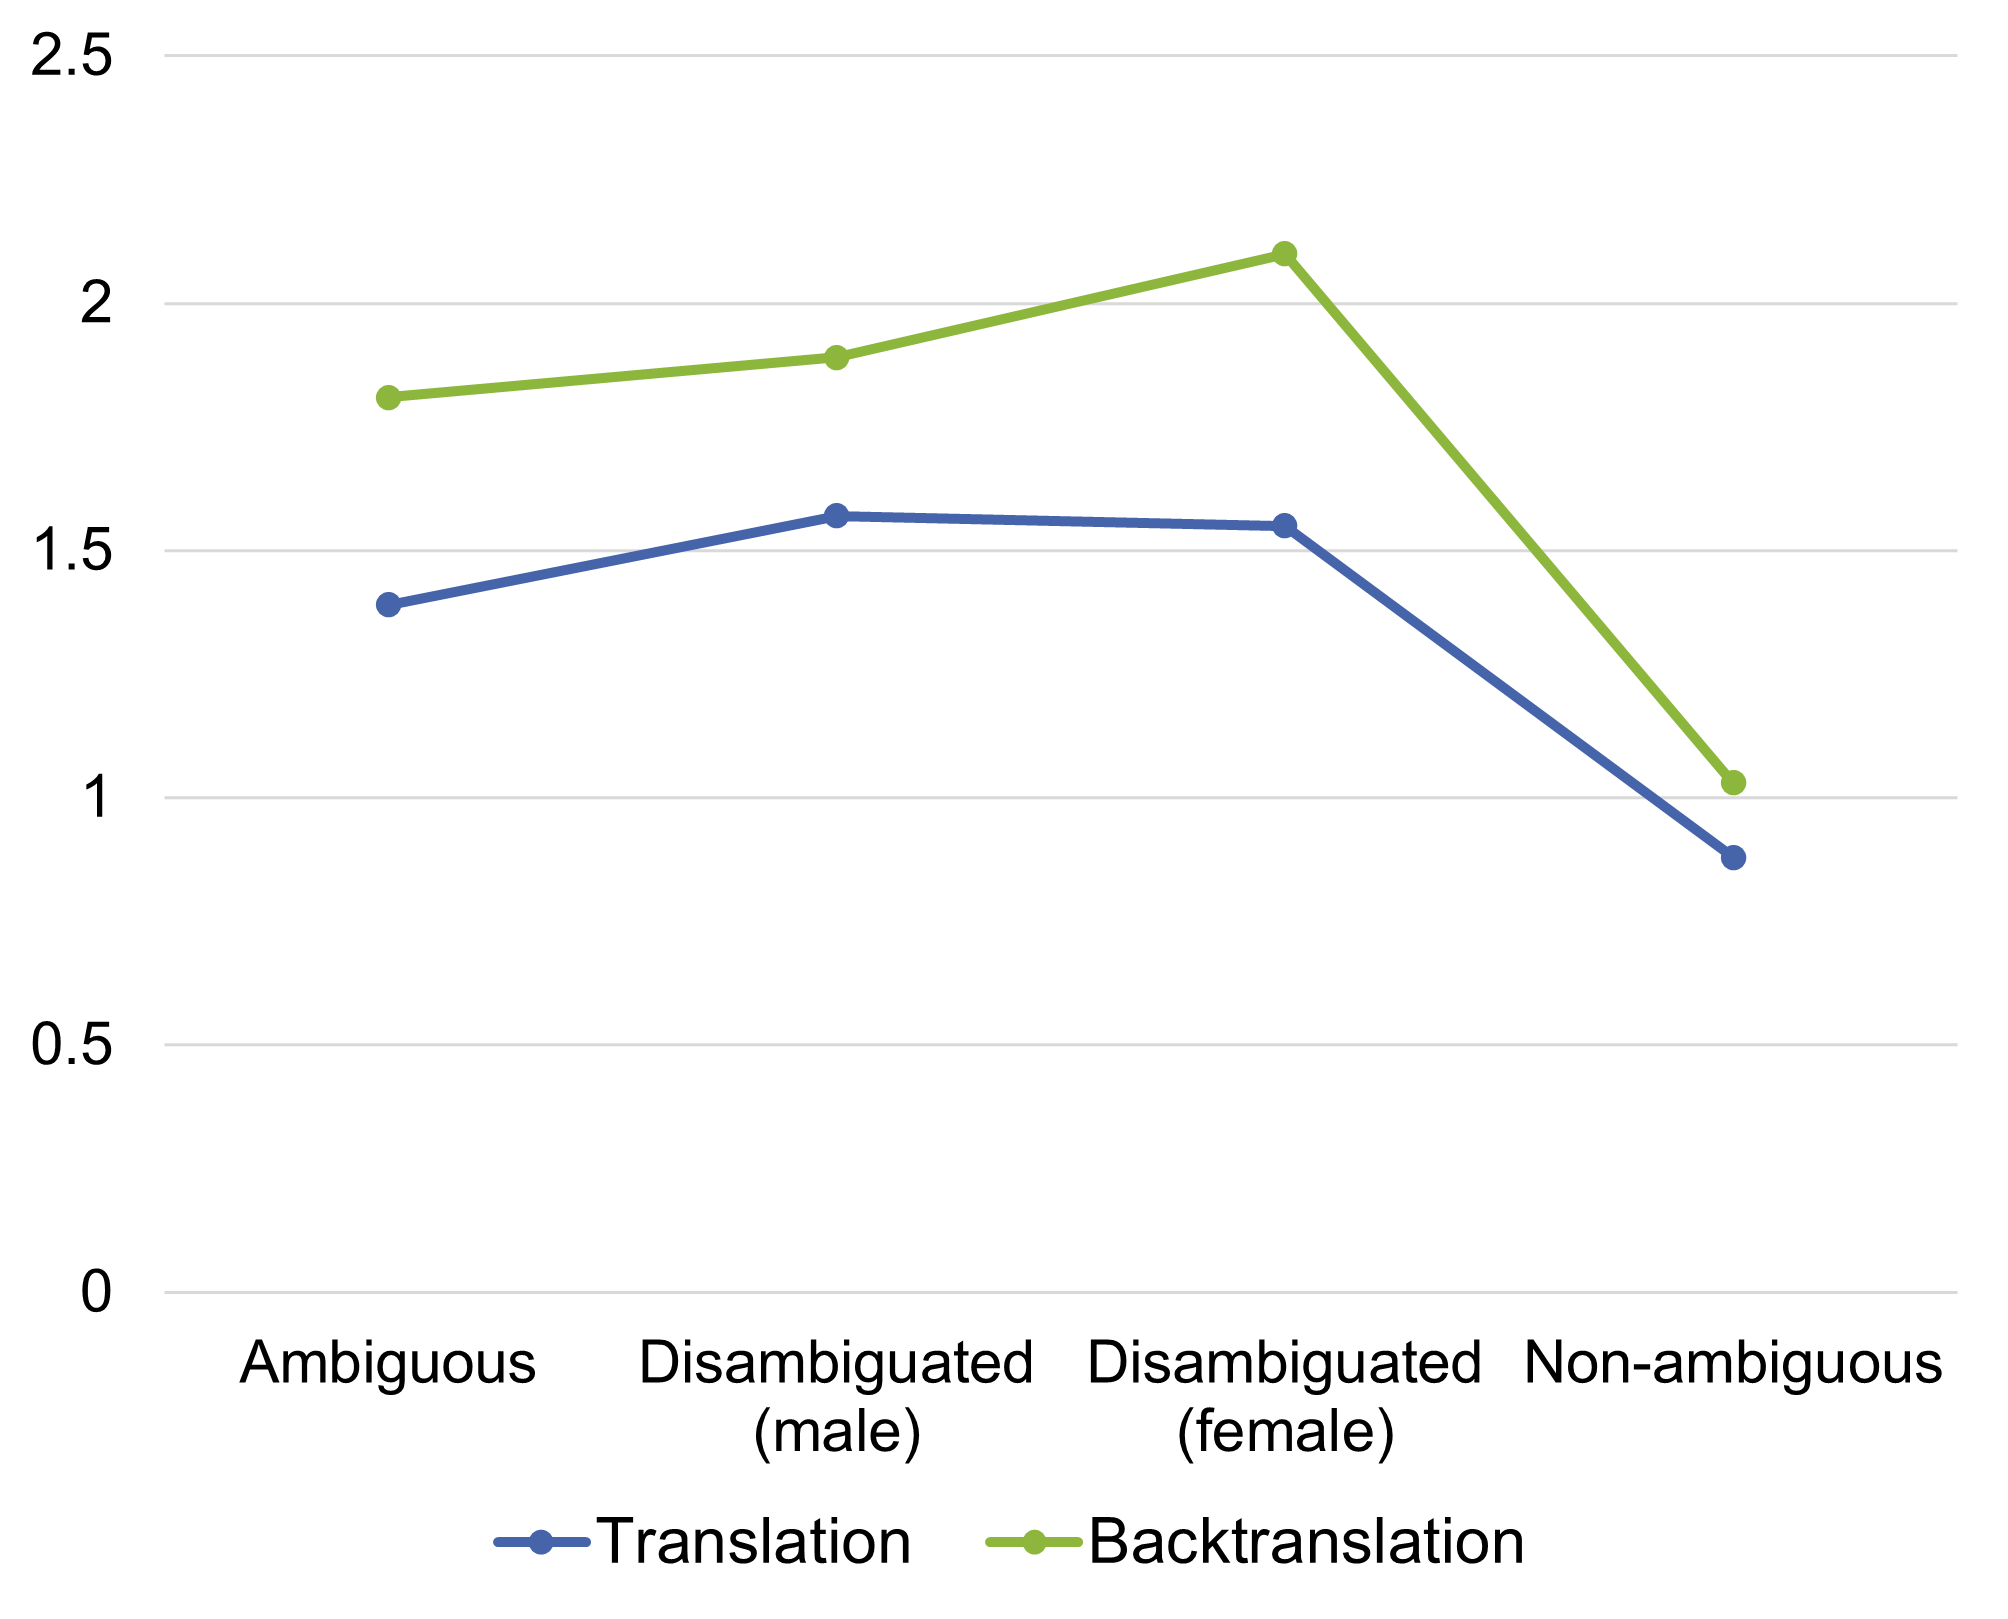
\includegraphics[width=\textwidth]{figures/correlation/words_beam10.png}
         \caption{Beam search with beam size 10}
         \label{fig:correlation_words_10}
     \end{subfigure}
     \hfill
     \begin{subfigure}{0.49\textwidth}
         \centering
         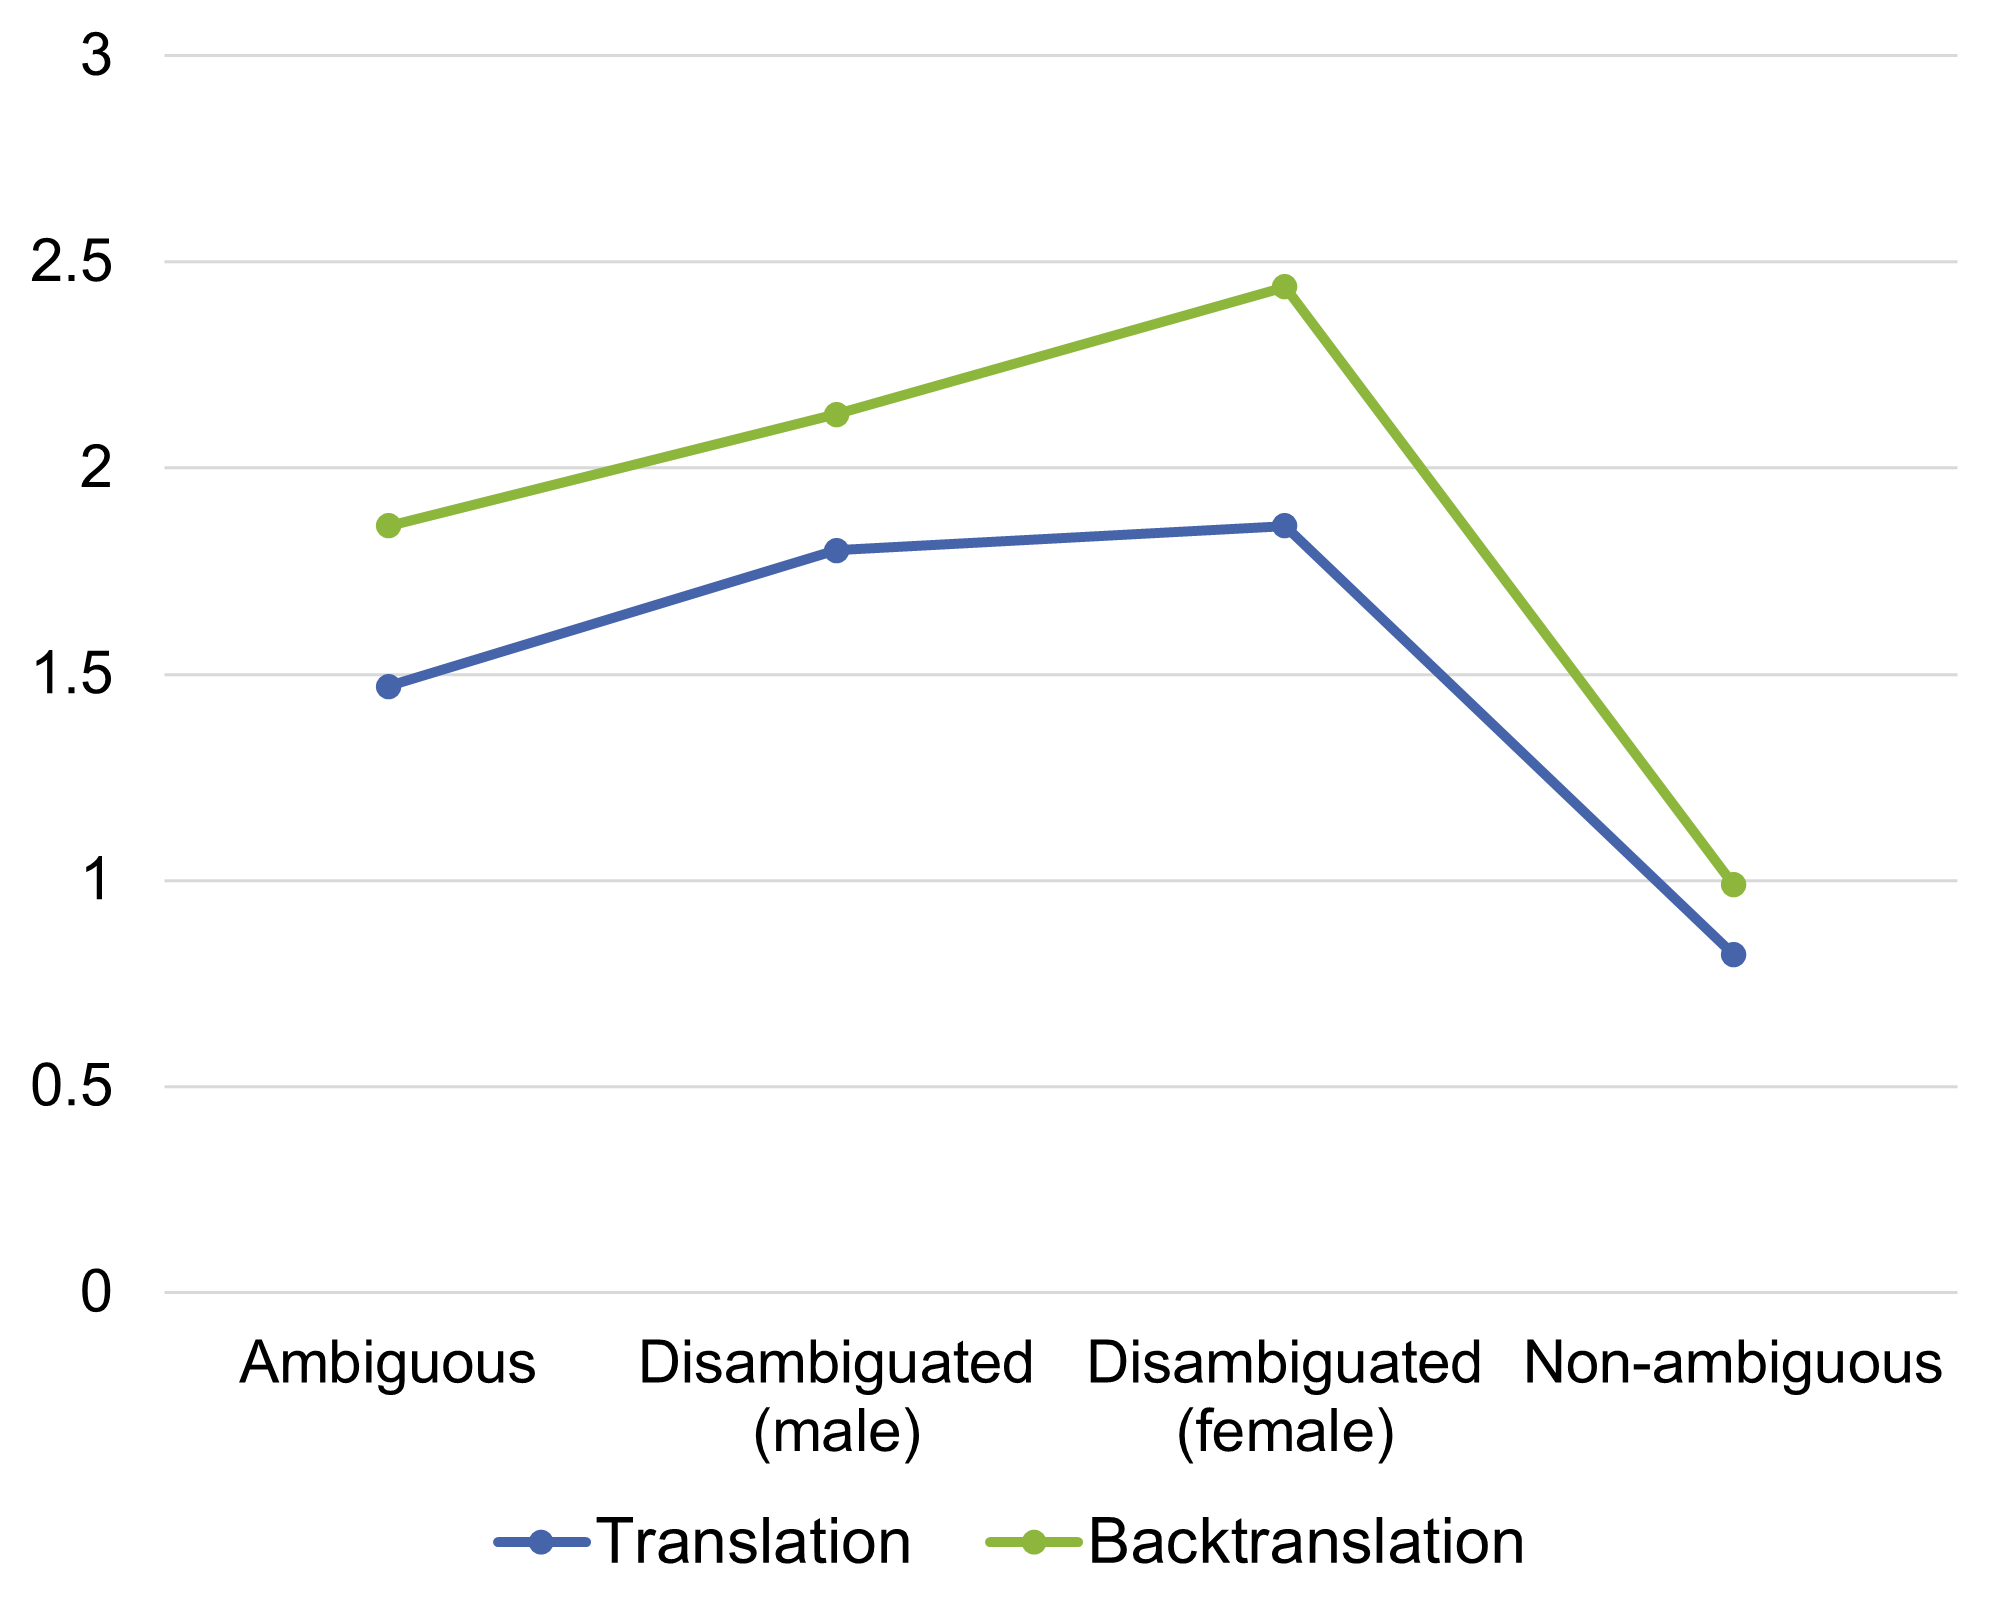
\includegraphics[width=\textwidth]{figures/correlation/words_sampling.png}
         \caption{Sampling}
         \label{fig:correlation_words_sampling}
     \end{subfigure}
     
    \caption{\textbf{Relationship Between Source Word and Rest of Sentence.} The results represent the amount of translations or backtranslations of the source word divided by the amount of translations or backtranslations of the rest of the sentence.}
    \label{fig:correlation_words}

\end{figure}
\chapter{Real-world Experiment}
\label{ch:Real_Experiment} 

This chapter describes an experiment in a real-world setting. The purpose of this experiment is to test the hypothesis in natural conditions. In the following, we outline the steps for executing the
experiment and the results from the evaluation.

%%%%%%%%%%%%%%%%%%%%%%%%%%%%%%%%%%%%%%%%%%%%%%%%%%%%%%%%%%%%%%%%%%%%%%%%%%%%%%%%%%%%%%%%%%%%
\section{Data Extraction}
\label{sec:Real_Experiment:Extraction}

First, we extract the natural sentences from the MuST-SHE corpus, as presented in Subsection \ref{sec:Setup:Natural_Corpora}. We choose 10 sentences for the experiment, that contain no context information regarding the gender of the ambiguous words. The sentence set is balanced, containing 3 sentences of each two genders - male and female. All sentences are listed in Table \ref{tab:mustshe_sentences}.

\begin{table} 
    \begin{tabularx}{\linewidth}{|X|l|l|}
        \hline
        \textbf{Source Sentence} & \textbf{Ambiguous Word(s)} & \textbf{Gender} \\ \hline
        So now Thomson becomes the more likely \textbf{suspect}. & suspect & male \\ \hline
        There was one black \textbf{professor} and one black assistant \textbf{dean}. & professor, dean & male \\ \hline
        We have our cognitive biases, so that I can take a perfect history on a \textbf{patient} with chest pain. & patient & male \\ \hline
        That's the \textbf{officer} who emailed me back, saying I think you can have a few classes with us.  & officer & male \\ \hline
        Steve, a physician, told me about a \textbf{doctor} that he worked with who was never very respectful, especially to junior staff and nurses. & doctor & male \\ \hline
        What do you think a batting average for a \textbf{cardiac surgeon} or a \textbf{nurse practitioner} or an \textbf{orthopedic surgeon}, an \textbf{OBGYN}, a \textbf{paramedic} is supposed to be? & \makecell[tl]{surgeon, \\ nurse practitioner, \\ OBGYN, paramedic} & female \\ \hline
        Fortunately for Mama Jane and her \textbf{friend}, a \textbf{donor} had provided treatment so that we could take them to the nearest hospital three hours away. & friend, donor & female \\ \hline
        The three words are: Do you remember? "Do you remember that patient you sent home?" the other \textbf{nurse} asked matter-of-factly. "Well she's back," in just that tone of voice. & nurse & female \\ \hline
        This one comes from a note that a \textbf{student} sent me after I gave a lecture about arousal nonconcordance. & student & female \\ \hline
        At the end of a conference in a hotel lobby once, I'm literally on my way out the door and a \textbf{colleague} chases me down. "Emily, I just have a really quick question."  & colleague & female \\ \hline
    \end{tabularx}
    \caption{\textbf{Extracted Natural Sentences.} MuST-SHE 4th Category: No gender-disambiguating information can be retrieved. 10 sentences in total.}
    \label{tab:mustshe_sentences}
\end{table}


%%%%%%%%%%%%%%%%%%%%%%%%%%%%%%%%%%%%%%%%%%%%%%%%%%%%%%%%%%%%%%%%%%%%%%%%%%%%%%%%%%%%%%%%%%%%
\section{Data Preprocessing}
\label{sec:Real_Experiment:Preprocessing}

As next, we preprocess the data by unmasking for each word in each original sentence. For unmasking we use the BERT base model, introduced in Section \ref{sec:Experiments:Tools}. The model generates five most probable words for each masked word. We replace the unmasked words in the sentences with three of the generated words. For each original sentence, we have three times the number of words in the sentence unmasked sentences.

\paragraph{Sets of Sentences} We have the following multiple sets of sentences:
\begin{itemize}
    \item Original set: the extracted sentences, as shown in Table \ref{tab:mustshe_sentences}. 
    \item Unmasked word sets: $3*|words|$ unmasked sentences for each sentences ($|words|$ denotes the number of words in the sentence)
\end{itemize}

\paragraph{Manual Replacement} Since very often the ambiguous words in the original sentences are unmasked with ambiguous words as well, we try to mitigate this by manually replacing the gender ambiguous noun words with the following non-ambiguous words: \textit{man, woman, girl, guy, boy}. We compare this approach with the originally replaced words by the BERT model.


%%%%%%%%%%%%%%%%%%%%%%%%%%%%%%%%%%%%%%%%%%%%%%%%%%%%%%%%%%%%%%%%%%%%%%%%%%%%%%%%%%%%%%%%%%%%
\section{Translation}
\label{sec:Real_Experiment:Translation}

We translate the sets of sentences from English to German in the two steps, also outlined in Section \ref{sec:Base_Experiment:Translation}:

\begin{enumerate}
    \item \textbf{Translation Source -> Target:} Translate the sets in the target language (German).
    \item \textbf{Backtranslation Target -> Source:} Translate the translations back into the source language (English).
\end{enumerate}

For translation, we use the Beam search decoding strategy (see Subsection \ref{sec:Background:Decoding}) with beam size 10. We choose this strategy based on the uniqueness evaluation results of the base experiment, where the number of unique sentences for the ambiguous subset is smaller than the number of unique sentences for the unambiguous subset, as expected.

%%%%%%%%%%%%%%%%%%%%%%%%%%%%%%%%%%%%%%%%%%%%%%%%%%%%%%%%%%%%%%%%%%%%%%%%%%%%%%%%%%%%%%%%%%%%
\section{Evaluation}
\label{sec:Real_Experiment:Evaluation}

For each original sentence, we execute the following algorithm:
\begin{enumerate}
    \item[1. ] Count the number of unique sentences in the backtranslations. \\
    $N \leftarrow |unique \; backtranslations|$ 
    \item[2. ] Count the number of unique sentences in the backtranslations for each unmasked word set of sentences. \\
    $w_{ij} \leftarrow |unique \; backtranslations \; for \; sentence \; with \; masked \; word \; w_{i} \; and \; mask \; j|$ \\
    $j \leftarrow \{1, 2, 3\}$ \\
    $i \leftarrow \{1, 2, ..., |words|\}$ \\
    $[w_{1j}, w_{2j}, ..., w_{|words|j}]$
    \item[3. ] Average the result for the three masks of each word. \\ 
    $w_{i}^{'} = \sum_{j=1}^{3} \frac{w_{ij}}{3} $ \\
    $[w_{1}^{'}, w_{2}^{'}, ..., w_{|words|}^{'}]$
    \item[4. ] Subtract the number of unique backtranslations of the original sentence from the average.
    $[|w_{1}^{'} - N|, |w_{2}^{'} - N|, ..., |w_{|words|}^{'} - N|]$ 
    \item[3.] Extract the words, which generate the 3 biggest differences. 
    
\end{enumerate}


Based on the Hypothesis \ref{a}, the original sentence containing an ambiguous word is expected to generate less unique sentences than the sentence with the corresponding unmasked ambiguous word, which is non-ambiguous. Therefore, this sentence is also expected to produce the biggest difference, when subtracting the number of unique sentences, pointing to the ambiguous word in the sentence. Since the natural sentences often exhibit more than one ambiguous word, we extract the three biggest differences, indicating three most ambiguous words in the original sentence.

%%%%%%%%%%%%%%%%%%%%%%%%%%%%%%%%%%%%%%%%%%%%%%%%%%%%%%%%%%%%%%%%%%%%%%%%%%%%%%%%%%%%%%%%%%%%
\section{Results}
\label{sec:Real_Experiment:Results}

The results from the evaluation can be seen in Table \ref{tab:mustshe_result}. We also compare the results of the replacement of the gender ambiguous nouns with BERT against the manual replacement. As we can see from the results, the manual replacement method achieves more detected ambiguous words in the list with the most probable ambiguous words. This proves that the theory of replacing ambiguous words with non-ambiguous words may help in detecting ambiguous words in a sentence. 


\begin{landscape} 
    \begin{tabularx}{\linewidth}{|>{\hsize=1\hsize}X|>{\hsize=0.6\hsize}X|>{\hsize=0.7\hsize}X|>{\hsize=0.7\hsize}X|}
        \hline
        \textbf{Source Sentence} & \textbf{Ambiguous Word(s)} & \textbf{BERT Replacement} & \textbf{Manual Replacement} \\ \hline
        
        So now Thomson becomes the more likely \textbf{suspect}. & suspect & [now, the, Thomson, \textbf{suspect}, more] & [now, the, Thomson, \textbf{suspect}, more] \\ \hline
        
        There was one black \textbf{professor} and one black assistant \textbf{dean}. & professor, dean & [\textbf{professor}, There, and, . , was] &  [\textbf{dean}, There, and, . , was] \\ \hline
        
        We have our cognitive biases, so that I can take a perfect history on a \textbf{patient} with chest pain. & patient & [cognitive, chest, a, history, I] & [cognitive, chest, a, history, I] \\ \hline
        
        That's the \textbf{officer} who emailed me back, saying I think you can have a few classes with us.  & officer & [classes, saying, . , you, can] & [classes, saying, . , can, \textbf{officer}] \\ \hline
        
        Steve, a physician, told me about a \textbf{doctor} that he worked with who was never very respectful, especially to junior staff and nurses. & doctor & [nurses, respectful, Steve, staff, especially] & [nurses, \textbf{doctor}, respectful, Steve, staff] \\ \hline
        
        What do you think a batting average for a \textbf{cardiac surgeon} or a \textbf{nurse practitioner} or an \textbf{orthopedic surgeon}, an \textbf{OBGYN}, a \textbf{paramedic} is supposed to be? & surgeon, nurse practitioner, OBGYN, paramedic & [think, an, for, or, be] & [\textbf{paramedic}, think, an, for, or] \\ \hline
        
        Fortunately for Mama Jane and her \textbf{friend}, a \textbf{donor} had provided treatment so that we could take them to the nearest hospital three hours away. & friend, donor & [the, we, three, , , a] & [the, we, three, , , a] \\ \hline
        
        The three words are: Do you remember? "Do you remember that patient you sent home?" the other \textbf{nurse} asked matter-of-factly. "Well she's back," in just that tone of voice. & nurse & [" , \textbf{nurse}, " , remember, of] & [" , \textbf{nurse}, " , remember, of] \\ \hline
        
        This one comes from a note that a \textbf{student} sent me after I gave a lecture about arousal nonconcordance. & student & [one, comes, nonconcordance, arousal, note] & [one, comes, nonconcordance, arousal, \textbf{student}] \\ \hline
        
        At the end of a conference in a hotel lobby once, I'm literally on my way out the door and a \textbf{colleague} chases me down. "Emily, I just have a really quick question."  & colleague & [chases, way, have, end, down] & [chases, way, have, end, down] \\ \hline
        
    \caption{\textbf{Natural Experiment Results.} Displays the 3 most ambiguous words (sorted in descending order) for each sentence generated according to the evaluation. The marked words are the expected ambiguous words. \\ BERT Replacement: Unmasking of each word with the BERT model. \\ Manual Replacement: Unmasking of the gender ambiguous nouns manually with non-ambiguous nouns.}
    \label{tab:mustshe_result}
    \end{tabularx}  
\end{landscape} 


%\chapter{Results}
\label{ch:Results}

% e.g. influence of language, context
\chapter{Discussion}
\label{ch:Discussion}

% Compare original test set with disambiguated test set:
% - How different are translations in each nbest backtranslation list?
% - Are they more different for sentences with unresolved ambiguity?

%%%%%%%%%%%%%%%%%%%%%%%%%%%%%%%%%%%%%%%%%%%%%%%%%%%%%%%%%%%%%%%%%%%%%%%%%%%%%%%%%%%%%%%%%%%%
\section{Summary of Results}
\label{sec:Discussion:Summary}


%%%%%%%%%%%%%%%%%%%%%%%%%%%%%%%%%%%%%%%%%%%%%%%%%
\subsection{Intraset Evaluation}
\label{sec:Discussion:Intraset}

%%%%%%%%%%%%%%%%%%%%%%%%%%%%%%%%%%%%%%%%%%%%%%%%%
\subsection{Interset Evaluation}
\label{sec:Discussion:Interset}


%%%%%%%%%%%%%%%%%%%%%%%%%%%%%%%%%%%%%%%%%%%%%%%%%%%%%%%%%%%%%%%%%%%%%%%%%%%%%%%%%%%%%%%%%%%%
\section{Answers to Research Questions}
\label{sec:Discussion:Answers}




%%%%%%%%%%%%%%%%%%%%%%%%%%%%%%%%%%%%%%%%%%%%%%%%%%%%%%%%%%%%%%%%%%%%%%%%%%%%%%%%%%%%%%%%%%%%
\section{Challenges and Limitations}
\label{sec:Discussion:Challenges}

% - Word alignment methods introduce errors, which influence the results
% - Not always having both genders present in the translation nbest list -> beam 100
% - Using “male” vs “female” for disambiguation yields different results
% -- NMT models bias leads to translation effects which in turn influence our method



% ? Subsection about open/unresolved questions
\chapter{Conclusion and Future Work}
\label{ch:Conclusion}

% take ideas for Future work from literature reviews and thesis


%% --------------------
%% |   Bibliography   |
%% --------------------

%% Add entry to the table of contents for the bibliography
\printbibliography[heading=bibintoc]

%% ----------------
%% |   Appendix   |
%% ----------------
\appendix
\iflanguage{english}
{\chapter{Appendix}}    % english style
{\chapter{Anhang}}      % german style
\label{chap:appendix}

%%%%%%%%%% Uniqueness distribution %%%%%%%%%%%%
\begin{figure}[!htb]
     \centering
     
     \begin{subfigure}{0.49\textwidth}
         \centering
         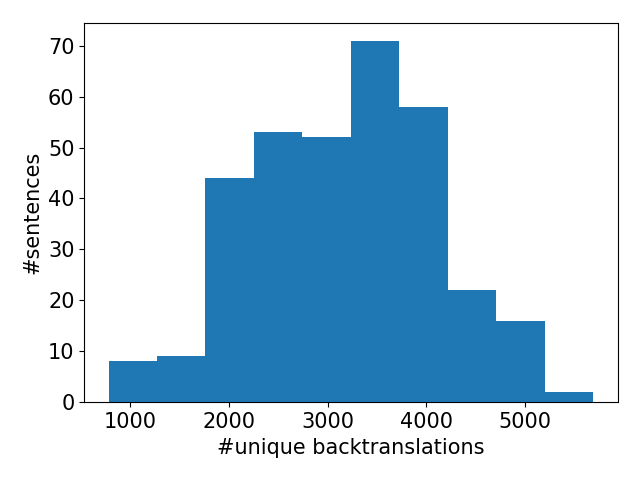
\includegraphics[width=\textwidth]{figures/uniqueness/unique_beam100/unique_back_original.png}
         \caption{Ambiguous Subset}
         %\label{fig:uniqueness_ambiguous}
     \end{subfigure}
     \hfill
     \begin{subfigure}{0.49\textwidth}
         \centering
         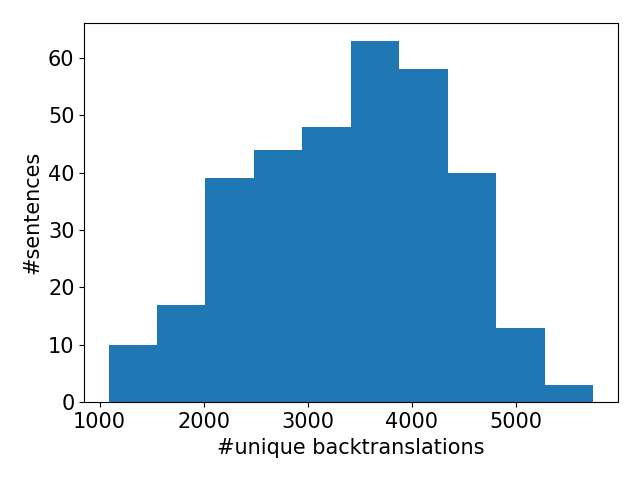
\includegraphics[width=\textwidth]{figures/uniqueness/unique_beam100/unique_back_male.png}
         \caption{Disambiguated Subset (male)}
         %\label{fig:uniqueness_male}
     \end{subfigure}
     \begin{subfigure}{0.49\textwidth}
         \centering
         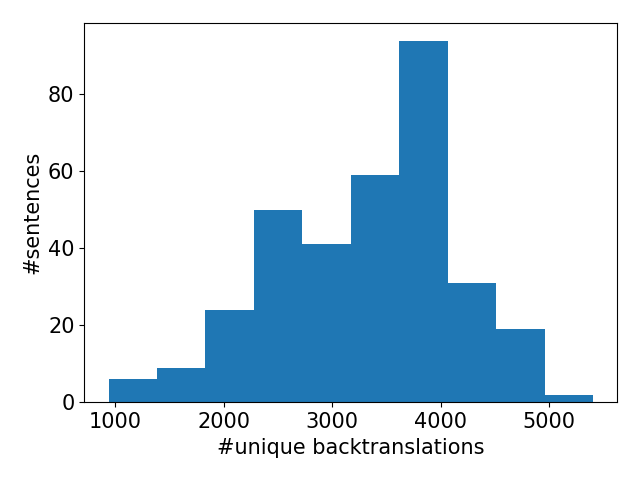
\includegraphics[width=\textwidth]{figures/uniqueness/unique_beam100/unique_back_average.png}
         \caption{Non-ambiguous Subset Average}
         %\label{fig:uniqueness_common}
     \end{subfigure}
     \hfill
     \begin{subfigure}{0.49\textwidth}
         \centering
         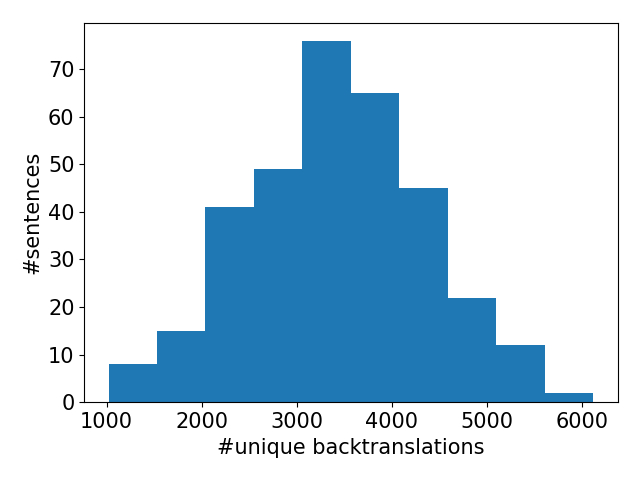
\includegraphics[width=\textwidth]{figures/uniqueness/unique_beam100/unique_back_female.png}
         \caption{Disambiguated Subset (female)}
         %\label{fig:uniqueness_female}
     \end{subfigure}
        \caption{Distribution of Unique Backtranslations: Beam search with beam size 100}
        \label{fig:uniqueness_graphs_100}

\end{figure}

\begin{figure}[!htb]
     \centering
     
     \begin{subfigure}{0.49\textwidth}
         \centering
         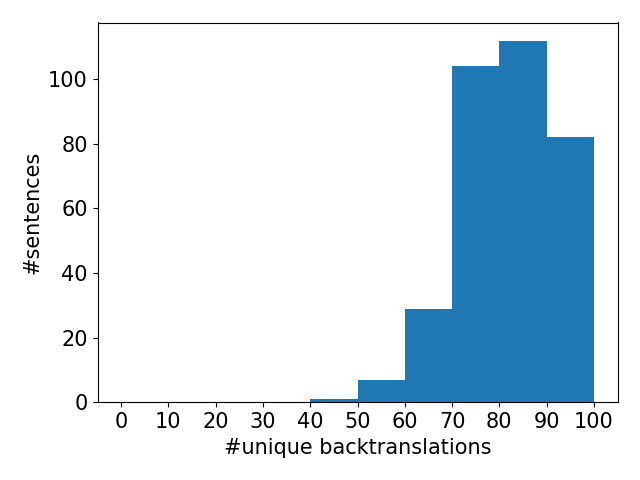
\includegraphics[width=\textwidth]{figures/uniqueness/unique_sampling/unique_back_original.png}
         \caption{Ambiguous Subset}
         %\label{fig:uniqueness_ambiguous}
     \end{subfigure}
     \hfill
     \begin{subfigure}{0.49\textwidth}
         \centering
         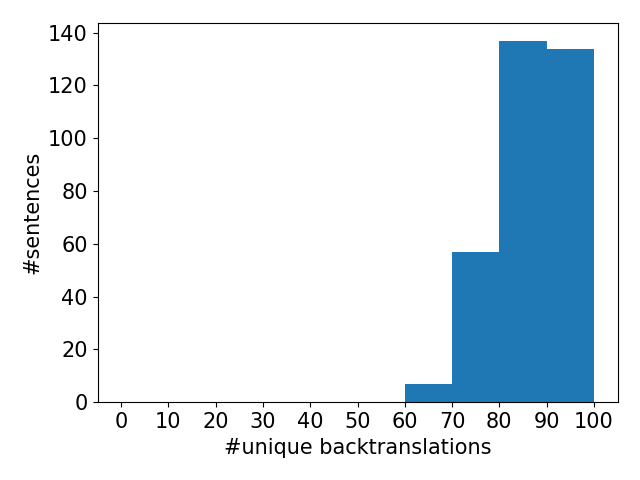
\includegraphics[width=\textwidth]{figures/uniqueness/unique_sampling/unique_back_male.png}
         \caption{Disambiguated Subset (male)}
         %\label{fig:uniqueness_male}
     \end{subfigure}
     \begin{subfigure}{0.49\textwidth}
         \centering
         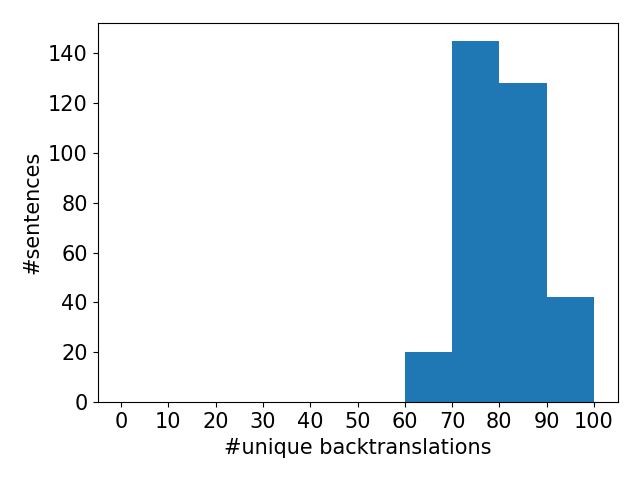
\includegraphics[width=\textwidth]{figures/uniqueness/unique_sampling/unique_back_average.png}
         \caption{Non-ambiguous Subset Average}
         %\label{fig:uniqueness_common}
     \end{subfigure}
     \hfill
     \begin{subfigure}{0.49\textwidth}
         \centering
         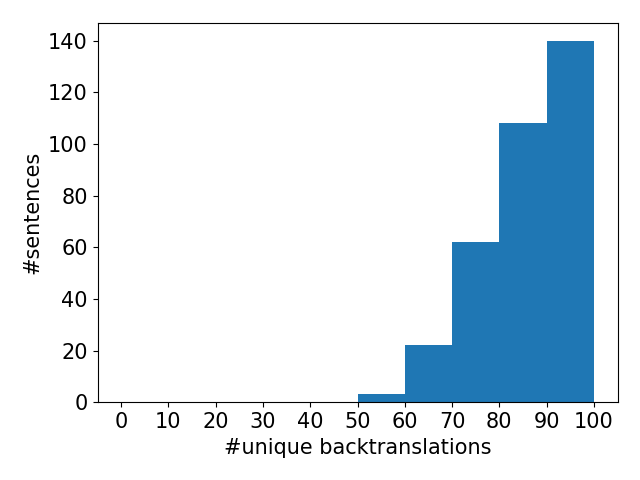
\includegraphics[width=\textwidth]{figures/uniqueness/unique_sampling/unique_back_female.png}
         \caption{Disambiguated Subset (female)}
         %\label{fig:uniqueness_female}
     \end{subfigure}
        \caption{Distribution of Unique Backtranslations: Sampling}
        \label{fig:uniqueness_graphs_sampling}

\end{figure}


%%%%%%%%%% Alignment distribution %%%%%%%%%%%%

% Beam 100
% Distribution for Translation
\begin{figure}[!htb]
     \centering
     
     \begin{subfigure}{0.49\textwidth}
         \centering
         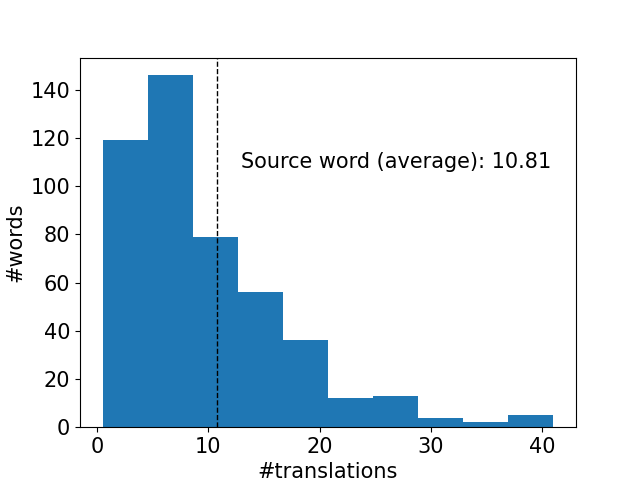
\includegraphics[width=\textwidth]{figures/alignment/align_100/word_translations_original.png}
         \caption{Ambiguous Subset}
         %\label{fig:alignment_translation_ambiguous}
     \end{subfigure}
     \hfill
     \begin{subfigure}{0.49\textwidth}
         \centering
         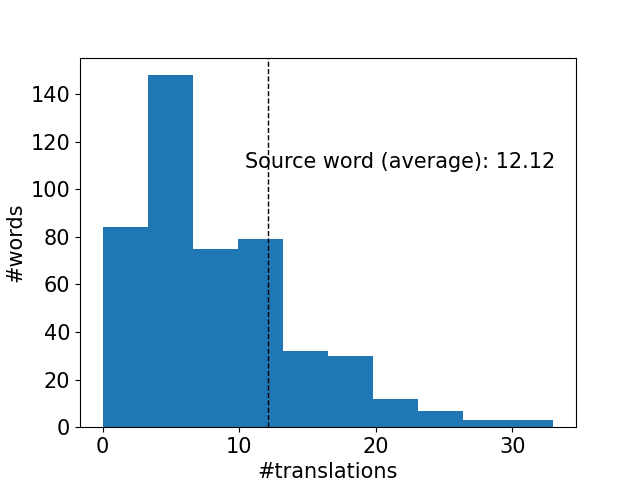
\includegraphics[width=\textwidth]{figures/alignment/align_100/word_translations_male.png}
         \caption{Disambiguated Subset (male)}
         %\label{fig:alignment_translation_male}
     \end{subfigure}
     \begin{subfigure}{0.49\textwidth}
         \centering
         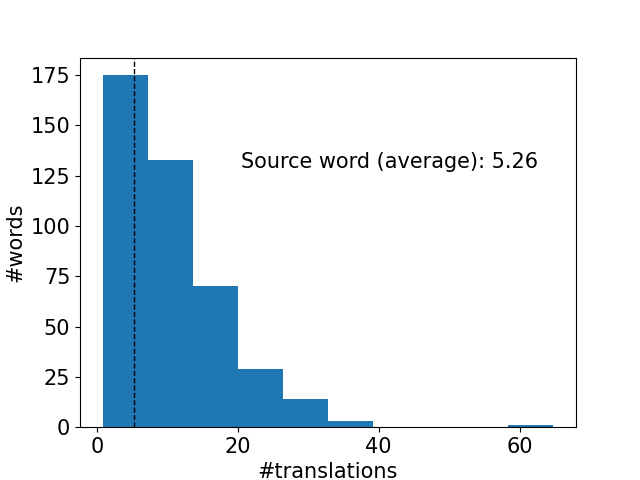
\includegraphics[width=\textwidth]{figures/alignment/align_100/word_translations_average.png}
         \caption{Non-ambiguous Subset Average}
         %\label{fig:alignment_translation_common}
     \end{subfigure}
     \hfill
     \begin{subfigure}{0.49\textwidth}
         \centering
         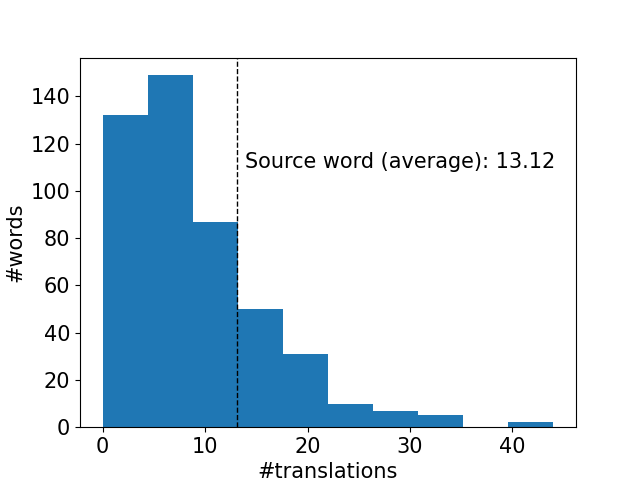
\includegraphics[width=\textwidth]{figures/alignment/align_100/word_translations_female.png}
         \caption{Disambiguated Subset (female)}
         %\label{fig:alignment_translation_female}
     \end{subfigure}
        \caption{\textbf{Distribution of Unique Translations for Words}. Beam search with beam size 100. Nbest size 100. Alignment with \textit{awesome-align}. The dashed line marks the average number of unique translations for the source word, the value displayed to the right.}
        \label{fig:alignment_graphs_translation_100}

\end{figure}

% Distribution for Backtranslation
\begin{figure}[!htb]
     \centering
     
     \begin{subfigure}{0.49\textwidth}
         \centering
         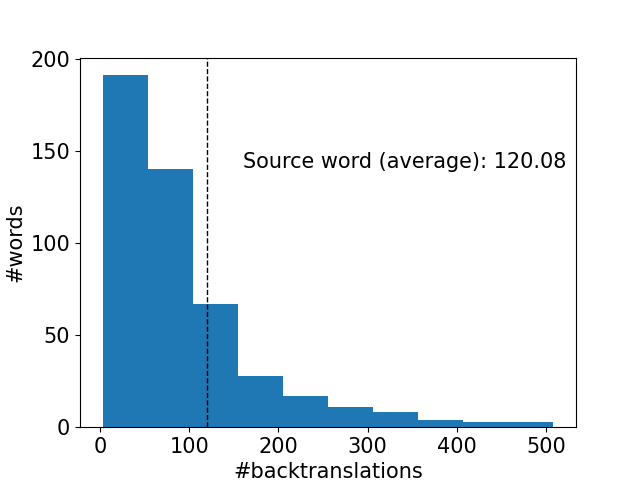
\includegraphics[width=\textwidth]{figures/alignment/align_100/word_backtranslations_original.png}
         \caption{Ambiguous Subset}
         %\label{fig:alignment_backtranslation_ambiguous}
     \end{subfigure}
     \hfill
     \begin{subfigure}{0.49\textwidth}
         \centering
         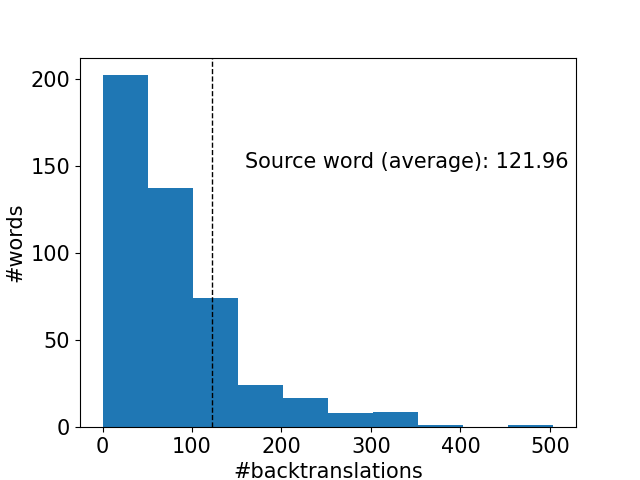
\includegraphics[width=\textwidth]{figures/alignment/align_100/word_backtranslations_male.png}
         \caption{Disambiguated Subset (male)}
         %\label{fig:alignment_backtranslation_male}
     \end{subfigure}
     \begin{subfigure}{0.49\textwidth}
         \centering
         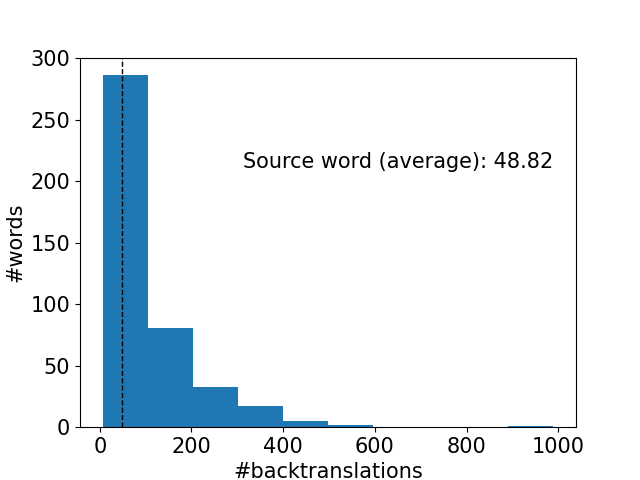
\includegraphics[width=\textwidth]{figures/alignment/align_100/word_backtranslations_average.png}
         \caption{Non-ambiguous Subset Average}
         %\label{fig:alignment_backtranslation_common}
     \end{subfigure}
     \hfill
     \begin{subfigure}{0.49\textwidth}
         \centering
         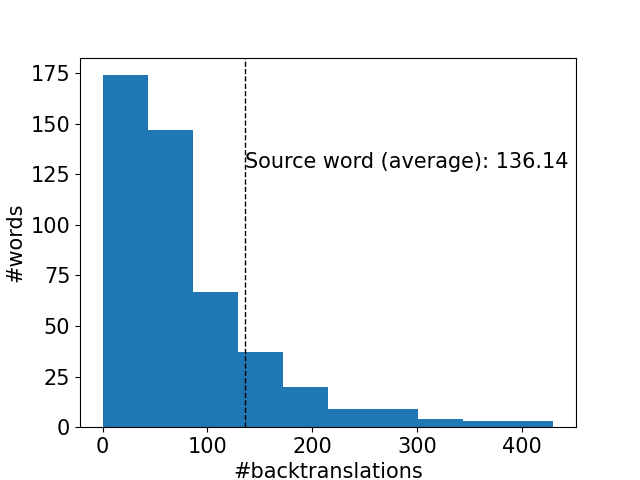
\includegraphics[width=\textwidth]{figures/alignment/align_100/word_backtranslations_female.png}
         \caption{Disambiguated Subset (female)}
         %\label{fig:alignment_backtranslation_female}
     \end{subfigure}
        \caption{\textbf{Distribution of Unique Backtranslations for Words}. Beam search with beam size 100. Nbest size 100. Alignment with \textit{awesome-align}. The dashed line marks the average number of unique translations for the source word, the value displayed to the right.}
        \label{fig:alignment_graphs_backtranslation_100}

\end{figure}

% Sampling
% Distribution for Translation
\begin{figure}[!htb]
     \centering
     
     \begin{subfigure}{0.49\textwidth}
         \centering
         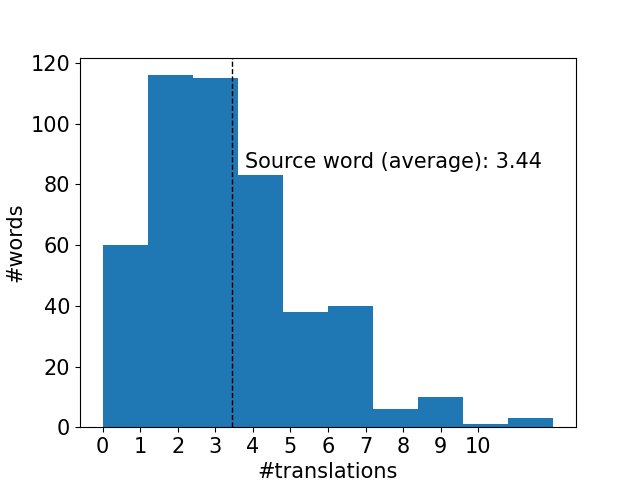
\includegraphics[width=\textwidth]{figures/alignment/align_sampling/word_translations_original.png}
         \caption{Ambiguous Subset}
         %\label{fig:alignment_translation_ambiguous}
     \end{subfigure}
     \hfill
     \begin{subfigure}{0.49\textwidth}
         \centering
         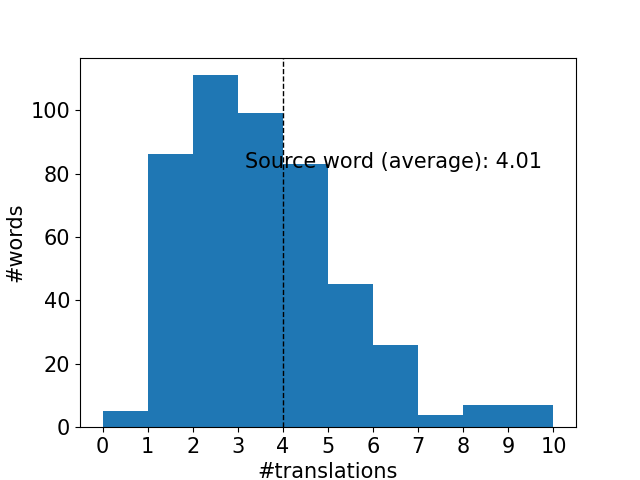
\includegraphics[width=\textwidth]{figures/alignment/align_sampling/word_translations_male.png}
         \caption{Disambiguated Subset (male)}
         %\label{fig:alignment_translation_male}
     \end{subfigure}
     \begin{subfigure}{0.49\textwidth}
         \centering
         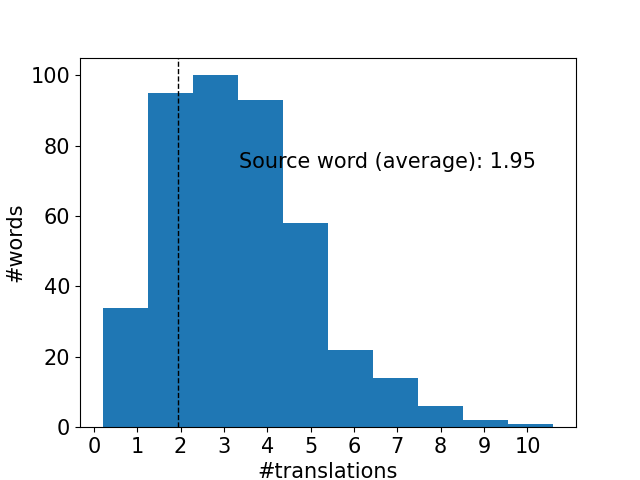
\includegraphics[width=\textwidth]{figures/alignment/align_sampling/word_translations_average.png}
         \caption{Non-ambiguous Subset Average}
         %\label{fig:alignment_translation_common}
     \end{subfigure}
     \hfill
     \begin{subfigure}{0.49\textwidth}
         \centering
         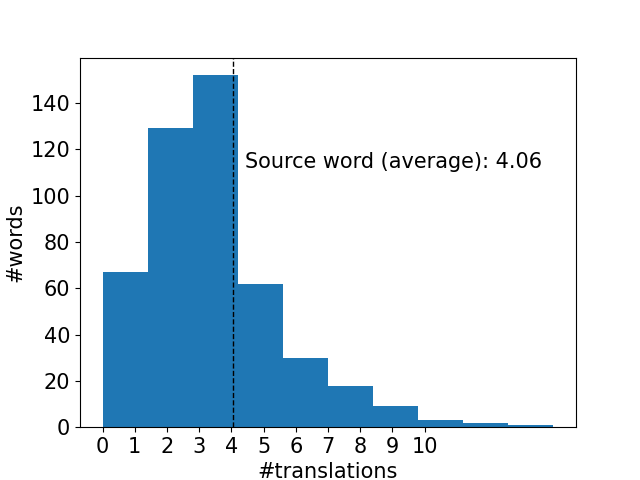
\includegraphics[width=\textwidth]{figures/alignment/align_sampling/word_translations_female.png}
         \caption{Disambiguated Subset (female)}
         %\label{fig:alignment_translation_female}
     \end{subfigure}
        \caption{\textbf{Distribution of Unique Translations for Words}. Sampling. Nbest size 10. Alignment with \textit{awesome-align}. The dashed line marks the average number of unique translations for the source word, the value displayed to the right.}
        \label{fig:alignment_graphs_translation_sampling}

\end{figure}

% Distribution for Backtranslation
\begin{figure}[!htb]
     \centering
     
     \begin{subfigure}{0.49\textwidth}
         \centering
         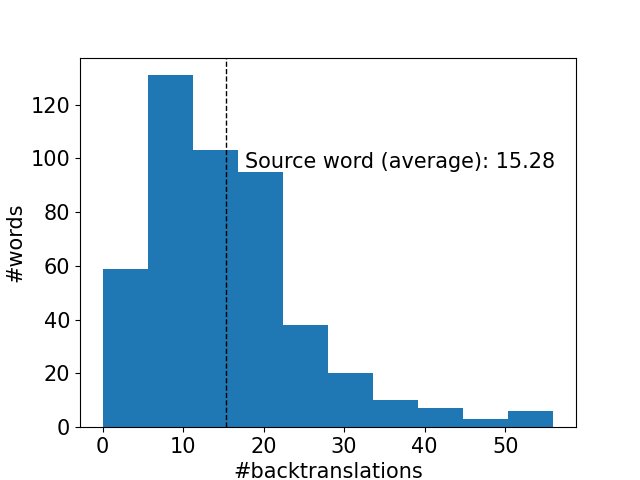
\includegraphics[width=\textwidth]{figures/alignment/align_sampling/word_backtranslations_original.png}
         \caption{Ambiguous Subset}
         %\label{fig:alignment_backtranslation_ambiguous}
     \end{subfigure}
     \hfill
     \begin{subfigure}{0.49\textwidth}
         \centering
         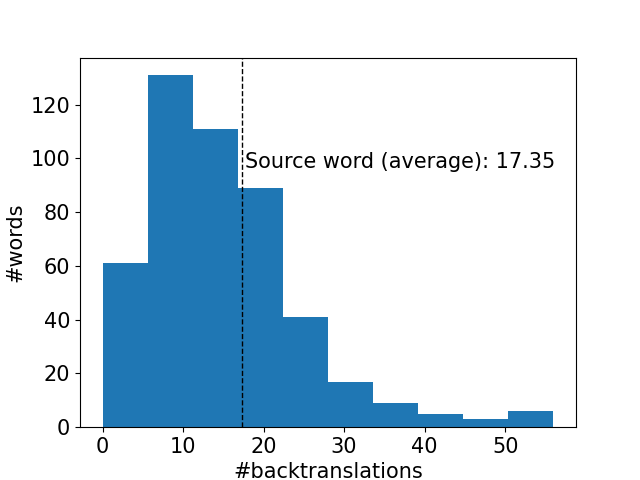
\includegraphics[width=\textwidth]{figures/alignment/align_sampling/word_backtranslations_male.png}
         \caption{Disambiguated Subset (male)}
         %\label{fig:alignment_backtranslation_male}
     \end{subfigure}
     \begin{subfigure}{0.49\textwidth}
         \centering
         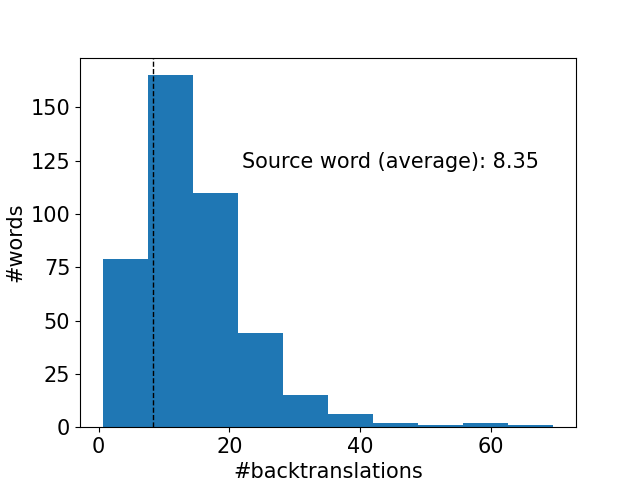
\includegraphics[width=\textwidth]{figures/alignment/align_sampling/word_backtranslations_average.png}
         \caption{Non-ambiguous Subset Average}
         %\label{fig:alignment_backtranslation_common}
     \end{subfigure}
     \hfill
     \begin{subfigure}{0.49\textwidth}
         \centering
         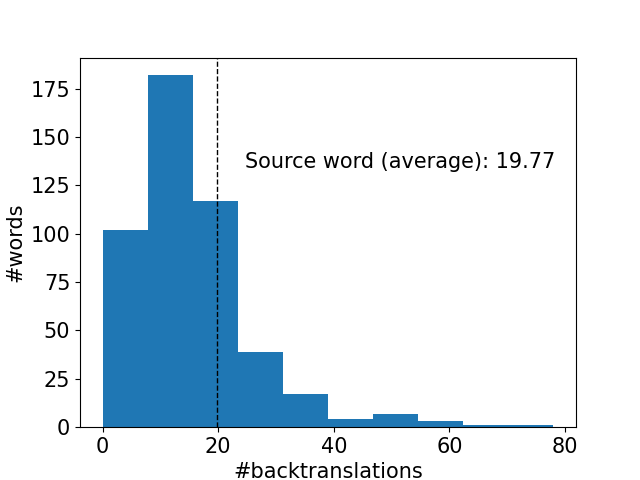
\includegraphics[width=\textwidth]{figures/alignment/align_sampling/word_backtranslations_female.png}
         \caption{Disambiguated Subset (female)}
         %\label{fig:alignment_backtranslation_female}
     \end{subfigure}
        \caption{\textbf{Distribution of Unique Backtranslations for Words}. Sampling. Nbest size 10. Alignment with \textit{awesome-align}. The dashed line marks the average number of unique translations for the source word, the value displayed to the right.}
        \label{fig:alignment_graphs_backtranslation_sampling}

\end{figure}

\end{document}
